%Modelo do esqueleto da dissertação
%Arquivo principal
\documentclass[espaco=umemeio,chapter=TITLE,twoside,openright]{abnt}
\usepackage{graphicx}
\usepackage[labelfont=bf]{caption}
\usepackage[utf8]{inputenc}
\usepackage[T1]{fontenc}
\usepackage{subcaption}
%\usepackage[latin1]{inputenc}
\usepackage{pifont} 
\usepackage{import}
\usepackage{amsmath}
\usepackage{multirow}
\usepackage{graphicx,url}
\usepackage{placeins}
\usepackage{adjustbox}
\usepackage[english]{babel}
\usepackage{lipsum}
\usepackage{multicol}
\usepackage{textcomp}
\usepackage{listings}
\usepackage[svgnames]{xcolor}
\usepackage[framemethod=TikZ]{mdframed}
\usepackage{caption}
\usepackage{amsmath}
\usepackage{calc}
\usepackage{array,url,kantlipsum}
\usepackage{algorithm}
\usepackage{algpseudocode}
\usepackage{lscape}
\usepackage{array}
\usepackage{longtable}
\usepackage[inline]{enumitem}
\usepackage{booktabs}
\usepackage{txfonts}
\usepackage{soul}
\usepackage{colortbl}%
  \newcommand{\myrowcolour}{\rowcolor[gray]{0.925}}
\newenvironment{Figure}
  {\par\medskip\noindent\minipage{\linewidth}}
  {\endminipage\par\medskip}

\lstset{
language=Java,
basicstyle=\small\ttfamily,
numbers=left,
numbersep=5pt,
xleftmargin=20pt,
frame=tb,
framexleftmargin=20pt
}

\renewcommand*\thelstnumber{\arabic{lstnumber}:}
\renewcommand{\abstractname}{\vspace{-\baselineskip}}

\DeclareCaptionFormat{mylst}{\hrule#1#2#3}
\captionsetup[lstlisting]{format=mylst,labelfont=bf,singlelinecheck=off,labelsep=space,font={normalsize,tt}}

\newlength{\Oldarrayrulewidth}
\newcommand{\Cline}[2]{%
  \noalign{\global\setlength{\Oldarrayrulewidth}{\arrayrulewidth}}%
  \noalign{\global\setlength{\arrayrulewidth}{#1}}\cline{#2}%
  \noalign{\global\setlength{\arrayrulewidth}{\Oldarrayrulewidth}}}

\newenvironment{bottompar}{\par\vspace*{\fill}}{\clearpage}



%\usepackage{suthesis-2e}

%\usepackage{algorithm} 
%\usepackage[cmex10]{amsmath}
%\usepackage{algpseudocode}
%\usepackage[brazil]{babel}
%\usepackage[utf8]{inputenc}
%\usepackage[T1]{fontenc}
%\usepackage{graphicx}
%\usepackage{longtable}
%\usepackage{multirow}
%\usepackage{rotating} 
%\usepackage{url}
%\usepackage[table]{xcolor}
\usepackage[alf]{abntcite}


\begin{document}

%Lista de definição de comandos a serem usados ao longo da tese, se for o caso
\newcommand{\beleleu}{\textit{beleleu}}


\begin{figure}
\centering

\includegraphics[scale=0.95]{logo.png}\\
\end{figure}

\autor{Francisco Nauber Bernardo Gois}

\titulo{Search-based Stress Test: an approach appling \\ evolutionary algorithms and trajectory methods}

\local{Fortaleza -- CE}

\data{September\,/\,2017}

\capa

%Modelo de folha de rosto

\begin{figure}
\centering

\includegraphics[scale=0.95]{logo.png}\\
\end{figure}

\autor{Francisco Nauber Bernardo Gois}

\titulo{Search-based Stress Test: an approach applying \\ evolutionary algorithms and trajectory methods}

\orientador[Thesis advisor: ]{Prof. Dr. Pedro Porfírio Muniz de Farias}



\coorientador[Thesis co-advisor: ]{Prof. Dr. André Luís Vasconcelos Coelho}

\comentario{A thesis
submitted to the Department of Applied Informatics (PPGIA) of Universidade de Fortaleza (UNIFOR), in partial fulfillment of the requirements for the degree of Doctor os Science in Applied Informatics.}


% \instituicao{Programa de Pós-Graduação em Informática Aplicada - PPGIA\par 
% 	Vice-Reitoria de Pesquisa e Pós-Graduação - VRPPG \par 
% 	Universidade de Fortaleza - UNIFOR \par
% 	Fundação Edson Queiroz}

\local{Fortaleza -- CE}

\data{September\,/\,2017}

\folhaderosto


%Modelo de folha de aprovação
%% não numerar a página!
\begin{folhadeaprovacao}

\begin{center}{\large Francisco Nauber Bernardo Gois}
 
\vspace{0.8in}
{\Large \textbf{Search-based Stress Test: an approach appyling \\ evolutionary algorithms and trajectory methods}}

\setlength{\ABNTsignthickness}{0.4pt}
\setlength{\ABNTsignwidth}{12cm}
\setlength{\ABNTsignskip}{1.5cm}

\vspace{0.7in}
Data de Aprova\c{c}\~ao: \underline{~~~~~}\,/\underline{~~~~~~~~~}

\vspace{0.5in}
Banca Examinadora:

\assinatura{D.Sc. Pedro Porfírio Muniz de Farias (UNIFOR)}

\assinatura{D.Sc. André Luís Vasconcelos Coelho (UNIFOR)}

\assinatura{D. Sc. Pedro de Alcantara dos Santos Neto
(UFPI)}

\assinatura{D. Sc. João Paulo Pordeus Gomes (UFC)}

\assinatura{Ph.D. Americo Tadeu Falcone Sampaio (UNIFOR)}

\assinatura{Docteur Napoleão Vieira Nepomuceno (UNIFOR)}

\end{center}

\end{folhadeaprovacao}





\vspace*{\fill}
\begin{quote} 
\centering 
    Learn from yesterday, live for today, hope for tomorrow. The important thing is not to stop questioning. 
    (Albert Einstein)
\end{quote}

\vspace*{\fill}


%Seção de agradecimentos
\chapter*{Acknowledgments} 

%\begin{trivlist} \itemsep 2ex \normalsize


It has been an exciting and instructive study period in the University of Fortaleza and I
feel privileged to have had the opportunity to carry out this study as demonstration of
knowledge gained during the period. With these acknowledgments, it would be impossible to remember those who in one way or another, directly or indirectly, have played a role in the realization of this research project. 

First of all, thank you God for the blessing and guiding me during all this project. I would like to dedicate this thesis to three of the most important people in my life
– my wife, my mother and my father – whose unconditional love and support gave me the
strength to follow my dream of becoming a scientist. I express all my gratitude to my beloved wife Najara, who endured five long years by my side without ever questioning my choice of becoming a doctor degree student. Thank you to my parents, Gois and Zirlanda,  for the example of life and for encouraging me as a child to enjoy science.

I would like to thank my very dedicated advisors Dr. Pedro Porfírio and André Coelho, for his guidance and support throughout this research project, which has been an excellent
learning experience for me. This thesis is not solely the product of my work but also the hard work and perseverance of my advisors, providing  help to keep me going even in the most difficult of times to get the project done. I could only hope that more students have the opportunity to work and learn from both professors like I did.

I also would like to thank the following people:

My thesis committee – Dr. Pedro de Alcantara dos Santos Neto, Dr. João Paulo Pordeus Gomes, Ph.D. Americo Tadeu Falcone Sampaio and Docteur Napoleão Vieira Nepomuceno – who made themselves available when I needed them to review previous drafts of this thesis and for their valuable suggestions that helped me to bring this work to its completion.

My family who loves me and are always present for good or bad: my mother in law Aroldina, my brothers Nilton and Nelio, my aunt Zena and my grandmother Elisabete.

Adriano Bessa, Victor and all professors from the post-graduate program for their direct and indirect contributions.

My colleagues from UNIFOR who supported me during this project: Adriana, Marum Simão, Celso Medeiros and José Renato. 

My company, SERPRO—Brazilian Federal Datacenter, for the (partial) financial support. My colleagues  Flavio Cysne, Fred Viana and Suderland Guimarães to help me with one of the experiments applied in this thesis. Sergio Gomes and Carlos Henrique (Managers of The Fortaleza Team) for giving me the time necessary to develop my activities.




%Seção de resumo

\begin{resumo} 
 
Alguns sistemas de software devem responder a milhares ou milhões de requisições simultâneos. Tais sistemas devem ser devidamente testados para garantir que eles possam funcionar corretamente sob uma carga esperada. Normalmente, a degradação do desempenho e conseqüentes falhas do sistema geralmente ocorrem em condições de estresse. No teste de estresse o sistema é submetido a cargas de trabalho acima dos resquistos não funcionais estabelecidos. Os testes de estresse diferem de outros tipos de testes em que o sistema é executado em seus pontos de interrupção, forçando o aplicativo ou a infra-estrutura de suporte a falhar. Testes de estressepodem ser vistos como um problema de otimização descontínuo, não-linear, com o domínio de entrada do sistema em teste como espaço de busca. Neste contexto, os testes baseados em busca (\textit{search-based tests}) são vistos como uma abordagem promissora para verificar as restrições de tempo. O teste de software baseado em busca é a aplicação de técnicas de pesquisa metaheurística para gerar testes de software. O critério de adequação do teste é transformado em uma função objetivo e um conjunto de soluções no espaço de busca é avaliado em relação à função objetivo usando uma metaheurística. O teste de estresse baseado em busca envolve encontrar os tempos de execução melhores e piores para verificar se as restrições de tempo são cumpridas. Os acordos de nível de serviço (SLA) são documentos que especificam garantias de desempenho realistas, bem como penalidades por incumprimento. Os SLAs são feitos entre provedores e clientes que incluem qualidade do serviço, capacidade de recursos, escalabilidade, obrigações e conseqüências em caso de violação. Satisfazer o SLA é de grande importância e um problema desafiador. A principal motivação desta tese é encontrar o tempo de resposta adequado dos SLAs usando teste de estresse. Esta tese apresenta três abordagens em testes de estresse baseados em busca. Primeiro, a metaheurística híbrida usa Tabu Search, Simulated Annealing e Algoritmos Genéticos de forma colaborativa. Em segundo lugar, uma abordagem chamada HybridQ usa uma técnica de aprendizado de reforço para otimizar a escolha de soluções vizinhas para explorar, reduzindo o tempo necessário para obter os cenários com o tempo de resposta mais longo na aplicação. As melhores soluções encontradas pelo HybridQ foram em média 5,98 \% melhores que alcançadas pela abordagem híbrida sem Q-learning. Em terceiro lugar, a tese investiga o uso dos algoritmos multi-objetivos NSGA-II, SPEA2, PAES e MOEA/D. A metaheurística MOEA/D obteve o melhor valor de hipervolume quando comparada com outras abordagens. A abordagem colaborativa usando MOEA/D e HybridQ melhora os valores de hipervolume obtidos e encontrou \textit{workloads} mais relevantes do que as experiências anteriores. Uma ferramenta chamada IAdapter, um plugin JMeter para realizar testes de esforço baseados em busca, foi desenvolvida e usada para realizar todas as experiências.

\textbf{Palavras-chave}: Search-based Testing, Stress Testing, Multi-objective metaheuristics, Hybrid metaheuristics, Reinforcement Learning.

\end{resumo}



%Resumo em inglês
\begin{abstract}

Some software systems must respond to thousands or millions of concurrent requests. These systems must be properly tested to ensure that they can function correctly under the expected load. Performance degradation and consequent system failures usually arise in stressed conditions. Stress testing subjects the program to heavy loads. Stress tests differ from other kinds of testing in that the system is executed on its breakpoints, forcing the application or the supporting infrastructure to fail. The search for the longest execution time is seen as a discontinuous, nonlinear, optimization problem, with the input domain of the system under test as a search space. In this context, search-based testing is viewed as a promising approach to verify timing constraints. Search-based software testing is the application of metaheuristic search techniques to generate software tests. The test adequacy criterion is transformed into a fitness function and a set of solutions in the search space are evaluated with respect to the fitness function using a metaheuristic. Search-based stress testing involves finding the best- and worst-case execution times to ascertain whether timing constraints are fulfilled. Service Level Agreements (SLAs)  are documents that specify realistic performance guarantees as well as
penalties for non-compliance.   SLAs are made between providers and customers that include service quality, resources
capability, scalability, obligations, and consequences in case of
violations. Satisfying SLA is of great importance and a challenging
issue. The main motivation of this thesis is define the response time of SLAs using Stress Testing. This thesis addresses the use of hybrid and multi-objective metaheuristics in conjunction with reinforcement learning techniques in search-based stress tests. A tool named IAdapter, a JMeter plugin for performing search-based stress tests, was developed.  The thesis uses Tabu Search, Simulated Annealing, and Genetic Algorithms in a collaborative manner. HybridQ uses a reinforcement learning technique to optimize the choice of neighboring solutions to explore, reducing the time needed to obtain the scenarios with the longest response time in the application.   Finally, the thesis investigates the use of the multi-objective algorithms in search-based stress testing. Several experiments were conducted to validate the proposed approach. The present research compared the proposed approach with other methods based on the use of single or multi-objective metaheuristics. The experiments showed a significant improvement in results with the Hybrid Metaheuristic approach. The best solutions found by HybridQ were on average 5.98\% better than that achieved by our previous approach without Q-learning. The use of multi-objective metaheuristics has made it possible to delimit a frontier where the response times are below the previously established service level. MOEA/D metaheuristics obtained the best hypervolume value when compared with other approaches. The collaborative approach using MOEA/D and HybridQ improves the hypervolume values obtained and found more relevant workloads than the previous experiments. More experimentation is also required to determine the most appropriate and robust parameters and verify changes related to the Pareto frontier in different executions. 



\textbf{Keywords}: Search-based Testing, Stress Testing, Multi-objective metaheuristics, Hybrid metaheuristics, Reinforcement Learning.
 
\end{abstract}
 


\tableofcontents

\listoffigures

\listoftables

 %Seção de acrônimos
\pretextualchapter{List of Acronyms}

\begin{description}
 \item BCET - Best-Case Execution Time .
 \item CP - Constraint Programming.
 \item GA - Genetic Algorithms.
 \item EMO - Evolutive Multi-objective algorithm.
 \item FOREPOST - Feedback-ORiEnted PerfOrmance Software Testing.
 \item HybridQ - Hybrid Metaheuristic with Q-Learning.
 \item ICA - Independent Component Analysis.
 \item MDP - Markov Decision Process.
 \item MOEA/D - Multiobjective Evolutionary Algorithm Based on Decomposition.
 \item MOEAs - Multi-objective evolutionary algorithms. 
 \item MOPs - Multi-objective problems. 
 \item NIST -  National Institute of Standards and Technology. 
 \item NSGA II - Non-dominated Sorting Genetic Algorithm II.
 \item P-metaheuristics - Population-based metaheuristics.
 \item PAES - Pareto Archived Evolution Strategy.
 \item PASA - A Method for Performance Assessment of Software Architectures.
 \item PID - Proportional,Integral, and Derivative.
 \item S-metaheuristic - Single Solution or Single-objective metaheuristic.
 \item SA - Simulated Annealing.
 \item SBSE - Search-based Software Engineering.
 \item SBST - Search-based Software testing. 
 \item SEDR - Standard Error Dynamic Resampling.
 \item SLAs - Service Level Agreements.
 \item SPEA2 - Strength Pareto Evolutionary Algorithm 2.
 \item TPC - Transaction Processing Performance.
 \item TS - Tabu Search.
 \item WCET - Worst-Case Execution Time .

 
\end{description}


\pretextualchapter{Glossary of Terms}

\begin{description}

\item EMOA package - R package design to  analysis of evolutionary multiobjective optimization algorithms.

\item IRace - Algorithm procedure to automatize the configuring parameters of metaheuristics \cite{ManuelLopez-IbanezJeremieDubois-LacosteLesliePerezCaceresMauroBirattari2016}.

\item Individual - In the context of evolutionary algorithms, individuals represent each solution found or used by the evolutionary algorithm \cite{GendreauMichelandPotvin2010}.

\item GUI objects - Graphical user interface elements are those elements used by graphical user interfaces to offer a consistent visual language. 

\item Offspring - New solutions created to new to a new generation in evolutionary algorithms\cite{GendreauMichelandPotvin2010}.

\item Outliers - An observation that is well outside of the expected range of values in a study or experiment, and which is often discarded from the data set \cite{GendreauMichelandPotvin2010}.

\item Pareto optimal-  Set of non-dominated solutions in a search-based problem \cite{deb2001multi}.

\item WorkLoad - Represents the size of the demand that will be imposed on the application under test in an execution. In this thesis, each workload represent an individual in the search space.


\end{description}

 
\pretextualchapter{Related Publications}

The following publications are related to this thesis:

\noindent \textbf{N. Gois, P. Porfirio and A. Coelho}. A multi-objective metaheuristic approach to search-based stress testing. In Proceedings of the 2017 IEEE International Conference on Computer and Information Technology (CIT), 2017 \cite{Gois2017}.

\noindent \textbf{N. Gois, P. Porfirio, A. Coelho, and T. Barbosa}. Improving Stress Search Based Testing using a Hybrid Metaheuristic Approach. In Proceedings of the 2016 Latin American Computing Conference (CLEI), pages 718–728, 2016 \cite{Gois2016}.


The following publications are submited and under review:

\noindent \textbf{N. Gois, P. Porfirio and A. Coelho}.Improving Search-Based Stress Testing Using Q-Learning and a Hybrid Metaheuristic Approach. Journal of Software Engineering Research and Development.



%\bibliographystyle{abnt-alf}
%\bibliography{bibliografia} %DESCOMENTAR



\chapter{Introduction}

\section{Motivation}

Performance problems such as high response times in software applications have a significant effect on the customers’  satisfaction. The explosive growth of the Internet has been instrumental in the increased need of applications that perform at an appropriate speed. Moreover, performance problems are often detected late in the application life cycle, and the later they are discovered, the greater the cost is to fix them. The use of stress testing is an increasingly common practice owing to the increasing number of users. In this scenario, the inadequate treatment of a workload,  generated by concurrent or simultaneous access due to several users, can result in highly critical failures and negatively affect the customers' perception of the company  \cite{Jiang2010} \cite{Molyneaux2009} \cite{Wert2014}.

Software testing is an expensive and difficult activity. The exponential
growth in the complexity of software makes the cost of testing continue to grow. Test case generation can be viewed as a search problem. The test adequacy criterion is transformed into a fitness function and a set of solutions in the search
space are evaluated with respect to the fitness function using a metaheuristic search technique. Search-based software testing is the application of metaheuristic search techniques to generate software
tests cases or perform test executions \cite{Afzal2009a}.

There is strong empirical evidence, that deficient
testing of both functional and non-functional properties
is one of the major sources of software and system errors. In 2002, NIST  report found that more than one-third of these costs of software failure could be eliminated by an improved testing infrastructure.
Automation of testing is a key concern. Through
automation, large-scale thorough testing can become
practical and scalable. However, automated generation of test cases presents challenges. The general problem involves finding a (partial) solution to the path sensitization problem. That is the problem of finding an input to drive the software down a chosen path \cite{Harman2010} \cite{dean2003managing}.

Software performance is a pervasive quality,  because it is influenced by every aspect of the design, code, and execution environment. Performance failures occur when a software product is not able to meet its overall objectives due to inadequate performance. Such failures negatively impact the projects by increasing costs, decreasing revenue or both \cite{Vetoio2011}. Stress testing of enterprise applications is manual, laborious, costly, and not particularly effective. When running many different test cases and observing application’s behavior, testers intuitively sense that there are certain properties of test cases that are likely to reveal performance bugs \cite{Grechanik2012}. Manual analysis of load testing is inefficient and error prone due to incomplete knowledge of test analyst about the application under test\cite{Arslan2015}.

Typically, stress testing is accomplished using test scripts, which are programs that test designers write to automate testing. These test scripts perform actions or mimicking user actions on GUI objects of the system to feed input data. Contemporary approaches to load testing suffer from limitations. Their cost-effectiveness depends heavily on the actual test scenarios that are used yet there is no support for choosing those scenarios. A poor choice of scenarios could lead to underestimating system response time thereby missing an opportunity to detect a performance problem \cite{Grechanik2012}.


Stress testing is an expensive and difficult activity. The exponential
growth in the complexity of software makes the cost of testing has only continued continued to grow. Test case generation can be seen as a search problem. The test adequacy criterion is transformed into a fitness function and a set of solutions in the search
space are evaluated with respect to the fitness function using a metaheuristic search technique. Search-based software testing is the application of metaheuristic search techniques to generate software
tests cases or perform test execution \cite{Afzal2009a}.

Search-based stress testing (SBST) is regarded as a promising approach to verify timing constraints \cite{Afzal2009a}. A common objective of a load search-based test is to find  scenarios that produce execution times that violate the specified timing constraints \cite{Sullivan}. 

Experimentation is essential in order to realistically and accurately evaluate search-based stress tests. Experimentation on algorithms is usually made by simulation. Experiments involving search-based stress tests are inherently complex and typically time-consuming and extremely difficult to repeat. Ordinarily, People who might want to duplicate published results, for example, must devote substantial resources to set up and the environmental conditions are likely to be different.

Usually, search-based test methods are based on a single objective optimization. Multi-objective evolutionary algorithms (MOEAs) are commonly used for solving multi-objective problems (MOPs) because they produce a complete set of solutions in a single run. Consequently, multi-objective heuristics may be more suitable in non-functional search-based tests, since these tests usually aim to obtain a result with more than one objective, for example, maximize the number of users of an application, minimizing your response time. 

Most of the commercial or academic tools don't use MOEAs in search-based stress tests. Several tools provide support for processing and running tests with different approaches. Moreover, while some of the tools use model-based tests, others set of tools use a scripting-based approach.Stress testing tools are essential in order to verify compliance with the service levels of an application.

Service Level is the service the customer hopes to receive \cite{Parasuraman1991}. Service Level Agreements (SLAs)  are documents that specify realistic performance guarantees as well as
penalties for non-compliance \cite{Menasce2002b}.   SLAs are made between providers and customers that include service quality, resources
capability, scalability, obligations and consequences in case of
violations. Satisfying SLA is very important and a challenging
issue \cite{Rajeshwari2016}. Decision making and definition of an SLA involve finding the appropriate response times for a test application. The main motivation of this thesis is to propose a new set of techniques that could help to define the response time of SLAs using search-based stress testing. The next sections introduce the Research Questions, Contributions and the Thesis Outline. 

\section{Research Questions}

This thesis addresses the use of hybrid and multi-objective metaheuristics in conjunction with reinforcement learning techniques in search-based stress tests. A tool named IAdapter (www.iadapter.org, github.com/naubergois/newiadapter), a JMeter plugin for performing search-based stress tests, was developed. The thesis uses a Noise Reduction algorithm named SEDR in the experiments of the chapter 6. Considering these motivations and the objective of this thesis, the main research questions which this thesis addresses are:

\begin{itemize}

\item \textbf{(Research Question 1)} How to improve the search for test scenarios in search-based stress testing using single-objective metaheuristics?

\item \textbf{(Research Question 2)} How to improve the choice of neighboring solutions in a single-objective metaheuristic to explore, reducing the time needed to obtain the scenarios with the longest response time in the application?

\item \textbf{(Research Question 3)} How to use multi-objective metaheuristics in search-based stress testing to obtain a Pareto frontier to improve the definition of SLAs?

\end{itemize}


In the next section, we show the main contributions of this thesis, based on the presented research questions.


\section{Contributions}

The main contributions of this thesis are follows:

\begin{itemize}
\item We propose a hybrid algorithm approach in search-based stress testing. The approach uses Tabu Search, Simulated Annealing and Genetic Algorithms. The thesis presents three experiments. The results were published in  \cite{Gois2016}. This proposal refers to our \textbf{Research Question 1} (Chapter 4).
 
\item We present a hybrid algorithm with the Q-Learning approach. The approach uses reinforcement learning to optimize the choice of neighboring solutions, reducing the time required to obtain the scenarios with the longest response time. This proposal refers to our \textbf{Research Question 2} (Chapter 5).

\item  We investigate the benefits of multiobjective metaheuristics in search-based stress testing. A comprehensive investigation of the use of multi-objective metaheuristics on search-based stress testing was conducted. Part of the results was published in \cite{Gois2017}.This proposal refers to our \textbf{Research Question 3} (Chapter 6).

\end{itemize}


The secondary contributions of this thesis are follows:

\begin{itemize}
\item The Survey of Stress Testing presented in Appendix A.
\item A Noise Reduction approach extended of the SEDR algorithm  presented in Appendix B.
\item The IAdapter tool presented in Appendix C.

\end{itemize}



\section{Thesis Outline}

The remainder of this thesis is organized as follows:

\textbf{Chapter 2} presents initial concepts about the use of metaheuristics, hybrid metaheuristics, multi-objective metaheuristics and reinforcement learning. The chapter briefly introduces the Trajectory and Population-based Metaheuristics.  Subsequently, presents Hybrid and Multi-Objective metaheuristics. Finally, presents the Reinforcement Learning concepts. 
\\

\textbf{Chapter 3} shows the context where this thesis is inserted and contemporary concepts about Search-based Stress Testing. In particular, two categories of approaches are out-lined: (i) Search-Based Stress Testing on Safety-critical systems; (ii) Search-Based Stress Testing on non Safety-critical systems.
\\

\textbf{Chapter 4} presents a hybrid approach that combines genetic algorithms, simulated annealing, and tabu search algorithms in stress tests. A tool named IAdapter, a JMeter plugin for performing search-based load tests, was developed. Three experiments  were performed to validate the proposed approach. The first experiment was performed on an emulated component, and the second one was performed using an installed Moodle application. The chapter presents the solution representation and the objective function of the proposed approach.
\\

\textbf{Chapter 5} presents a reinforcement learning approach to optimize the choice of neighboring solutions to explore, reducing the time needed to obtain the scenarios with the longest response time in the application. The chapter presents a study that extends the article "Improving stress search based testing using a hybrid metaheuristic approach"  in order to ascertain if the use of the Q-learning technique allows the meta-heuristic algorithms to improve the search to application failures with a smaller number of requests consuming a shorter time assuming that the same application can be submitted to more than one test execution.
\\

\textbf{Chapter 6} presents experiments to assert the benefits of multiobjective metaheuristics in search-based stress testing. The first experiment uses NSGA-II algorithm to discover application scenarios where there is a high response time for a small number of users. The second experiment presents the experimental results to compare four multi-objective algorithms in search-based stress testing. The third experiment shows the results conducted to compare the MOEA/D multi-objective with the HybridQ algorithm.  The fourth experiment presents an experiment to evaluate the collaborative approach using HybridQ and MOEA/D. Finally, we present an initial study to evaluate the Pareto Frontier difference in multiple executions. 

\chapter{Metaheuristics and Reinforcement Learning}

This chapter presents concepts and essentials definitions considering the main contributions of this thesis: the single and multi-objective metaheuristics and reinforcement learning. 

\section{Metaheuristics}

Metaheuristics are strategies that guide the search process to efficiently explore the search space in order to find optimal solutions. Metaheuristic algorithms are approximate and usually non-deterministic and sometimes incorporate mechanisms to avoid getting trapped in confined areas of the search space. There are different ways to classify and describe metaheuristic algorithm \cite{Blum2003}:

\begin{itemize}
\item Nature-inspired vs. non-nature inspired. There are nature-inspired algorithms, like Genetic Algorithms and Ant Algorithms, and non nature-inspired ones such as Tabu Search and Iterated Local Search.

\item Population-based vs. single point search (Trajectory methods). Algorithms working on single solutions are called trajectory methods, like Tabu Search, Iterated Local Search and Variable Neighborhood Search. They all share the property of describing a trajectory in the search space during the search process. Population-based metaheuristics perform search processes which describe the evolution of a set of points in the search space.

\item One vs. various neighborhood structures. Most metaheuristic algorithms work on one single neighborhood structure. In other words, the fitness landscape topology does not change in the course of the algorithm. Other metaheuristics, such as Variable Neighborhood Search (VNS), use a set of neighborhood structures which gives the possibility to diversify the search by swapping between different fitness
landscapes.


\end{itemize}

\subsection{Trajectory Methods}

Trajectory methods are characterized by a trajectory in the search space. Two common trajectory methods are Simulated Annealing and Tabu Search.

\subsubsection{Neighborhood}

The definition of Neighborhood is a required common step in the design of any Single-Solution metaheuristic (S-metaheuristic). The neighborhood structure it is an important piece of the performance of an S-metaheuristic. If the neighborhood structure is not adequate to the problem,
any S-metaheuristic will fail to solve the problem. The neighborhood function N is a mapping: $ N : S \rightarrow N\textsuperscript{2} $ that assigns to each solution s of \textit{S} a set of solutions \textit{N(s)}$\subset$ S \cite{Talbi2013}.

The neighborhood definition depends  representation associated with the problem. For permutation-based representations, a usual neighborhood is based on the swap operator that consists in swapping the location of two elements $s_i$ and $s_j$ of the permutation \cite{Talbi2013}. The Fig. \ref{fig:sperneighborhood} presents an example where a set of neighbors is found by permutation.


\begin{figure}[h]
\centering
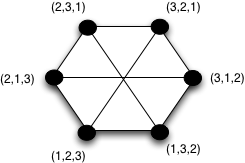
\includegraphics[width=0.5\textwidth]{./images/neighborhood.png}
\caption{ An example of neighborhood for a permutation \cite{Talbi2013}.}
\label{fig:sperneighborhood}
\end{figure}



Single-Solution Based Metaheuristics methods are characterized by a trajectory in the search space. Two common S-metaheuristics methods are Simulated Annealing and Tabu Search.

\subsubsection{Simulated Annealing}

The algorithmic framework of SA is described in Alg. \ref{sa}.  The algorithm starts by generating an initial solution in function \textit{GenerateInitialSolution()}. The initial temperature value is determined in function \textit{SetInitialTemperature()} such that the probability for an uphill move is quite high at the start of the algorithm. At each iteration a solution $\mbox{s}_1$ is randomly chosen in function \textit{PickNeighborAtRandom(N(s))}. If \textit{$\mbox{s}_1$} is better than \textit{s}, then \textit{$\mbox{s}_1$} is accepted as a new current solution. Else, if the move from \textit{s} to \textit{$\mbox{s}_1$} is an uphill move, \textit{$\mbox{s}_1$}  is accepted with a probability which is a function of a temperature parameter \textit{Tk} and \textit{s} \cite{raidl2010metaheuristic}.

\begin{algorithm}[t]
  \caption{Simulated Annealing Algorithm}\label{sa}
  \begin{algorithmic}[1]

    \State $s\gets GenerateInitialSolution()$
    \State $k\gets 0 $
    \State $Tk\gets SetInitialTemperature()$
    \While{termination conditions not met }
    \State $\mbox{s}_1\gets PickNeighborAtRandom(N (s))$
    \If{$(f(\mbox{s}_1)<f(s))$}
    \State $s\gets\mbox{s}_1$
    \Else $\;$ Accept $\mbox{s}_1$ as new solution with probability p($\mbox{s}_1|$Tk,s)
    \EndIf
    \State $K\gets K+1$
    \State $Tk\gets AdaptTemperature()$
    \EndWhile

  \end{algorithmic}
\end{algorithm}

\subsubsection{Tabu Search}

Tabu Search uses a tabu list to keep track of the last  moves, and don’t allow going back to these \cite{Glover1986}. The algorithmic framework of Tabu Search is described in Alg. \ref{tsa}.  The algorithm starts by generating an initial solution in function \textit{GenerateInitialSolution()} and the tabu lists are initialized as empty lists in function \textit{InitializeTabuLists($\mbox{TL}_1$,...,$\mbox{TL}_r$)}. For performing a move, the algorithm first determines those solutions from the neighborhood \textit{N(s)} of the current solution \textit{s} that contain solution features currently to be found in the tabu lists. They are excluded from the neighborhood, resulting in a restricted set of neighbors \textit{$\mbox{N}_a(s)$}. At each iteration, the best solution \textit{$\mbox{s}_1$} from \textit{$\mbox{N}_a(s)$} is chosen as the new current solution. Furthermore, in procedure \textit{UpdateTabuLists($\mbox{TL}_1$,...,$\mbox{TL}_r$,s,$\mbox{s}_1$)} the corresponding features of this solution are added to the tabu lists.


\begin{algorithm}[t]
  \caption{Tabu Search Algorithm}\label{tsa}
  \begin{algorithmic}[2]

    \State $s\gets GenerateInitialSolution()$
    \State InitializeTabuLists($\mbox{TL}_1$,...,$\mbox{TL}_r$)
    \While{termination conditions not met }
    \State $\mbox{N}_a(s)\gets$ $\{\mbox{s}_1 \in N(s) |\mbox{s}_1$ does not violate a tabu condition, or it satisfies at least one aspiration condition $\}$
    \State $\mbox{s}_1\gets argmin\{f(\mbox{s}_2)|\mbox{s}_2 \in \mbox{N}_a(s) \}$
    \State UpdateTabuLists($\mbox{TL}_1$,...,$\mbox{TL}_r$,s,$\mbox{s}_1$)
    \State $s\gets \mbox{s}_1$
    \EndWhile

  \end{algorithmic}
\end{algorithm}

\subsection{Population-based Metaheuristics}

Population-based metaheuristics (P-metaheuristics) could be viewed as an iterative improvement in a population of solutions. First, the population is initialized. Then, a new population of solutions is generated. Finally, this population is integrated into the current one using  selection procedures. The search process is stopped when a stopping criterion is satisfied. Algorithms such as Genetic algorithms (GA), scatter search (SS), estimation of distribution algorithms (EDAs), particle swarm optimization (PSO), bee colony (BC), and artificial immune systems (AISs) belong to this class of metaheuristics \cite{talbi2009metaheuristics}.

Population-based metaheuristics are comprised of several components \cite{hong2000simultaneously} \cite{shousha2003performance} :

\begin{itemize}
\item a representation of the solution, referred as the chromosome;
\item fitness of each chromosome, referred as objective function;
\item the genetic operations of crossover and mutation which generate new offspring.
\end{itemize}

The crossover operation or recombination recombines two or more individuals to produce new individuals. Mutation or modification operators causes a self-adaptation of individuals \cite{Blum2003}. In Search-based tests, the crossover operator creates two new test cases T1' and T2' by combining test cases from two pre-existing test cases T1 and T2 \cite{Aleti2016}. Algorithm \ref{gna} shows the basic structure of GA algorithms. In this algorithm, P denotes the population of individuals. A population of offspring is generated by the application of recombination and mutation operators and the individuals for the next population are selected from the union of the old population and the offspring population \cite{raidl2010metaheuristic}.


\begin{algorithm}[h]
  \caption{Genetic Algorithm}\label{gna}
  \begin{algorithmic}[1]

    \State $s\gets GenerateInitialSolution()$
    \State Evaluate(P)
    \While{termination conditions not met }
    \State $\mbox{P}_1\gets$ $Recombine(P)$
    \State $\mbox{P}_2\gets$ $Mutate(\mbox{P}_1)$
    \State $Evaluate(\mbox{P}_2)$
    \State $P\gets Select(\mbox{P}_2,P)$
    \EndWhile

  \end{algorithmic}
\end{algorithm}


\subsection{Hybrid  Metaheuristics}

A combination of one metaheuristic with components from other metaheuristics is called a hybrid metaheuristic. The concept of hybrid metaheuristics has been commonly accepted only in recent years, even if the idea of combining different metaheuristic strategies and algorithms dates back to the 1980s. Today, we can observe a generalized common agreement on the advantage of combining components from different search techniques and the tendency of designing hybrid techniques is widespread in the fields of operations research and artificial intelligence \cite{raidl2010metaheuristic}.


There are two main categories of metaheuristic combinations: collaborative combinations and integrative combinations. These are presented in Fig. \ref{fig:metaheuristc} \cite{Raidl2006}.

\begin{figure}[h]
\centering
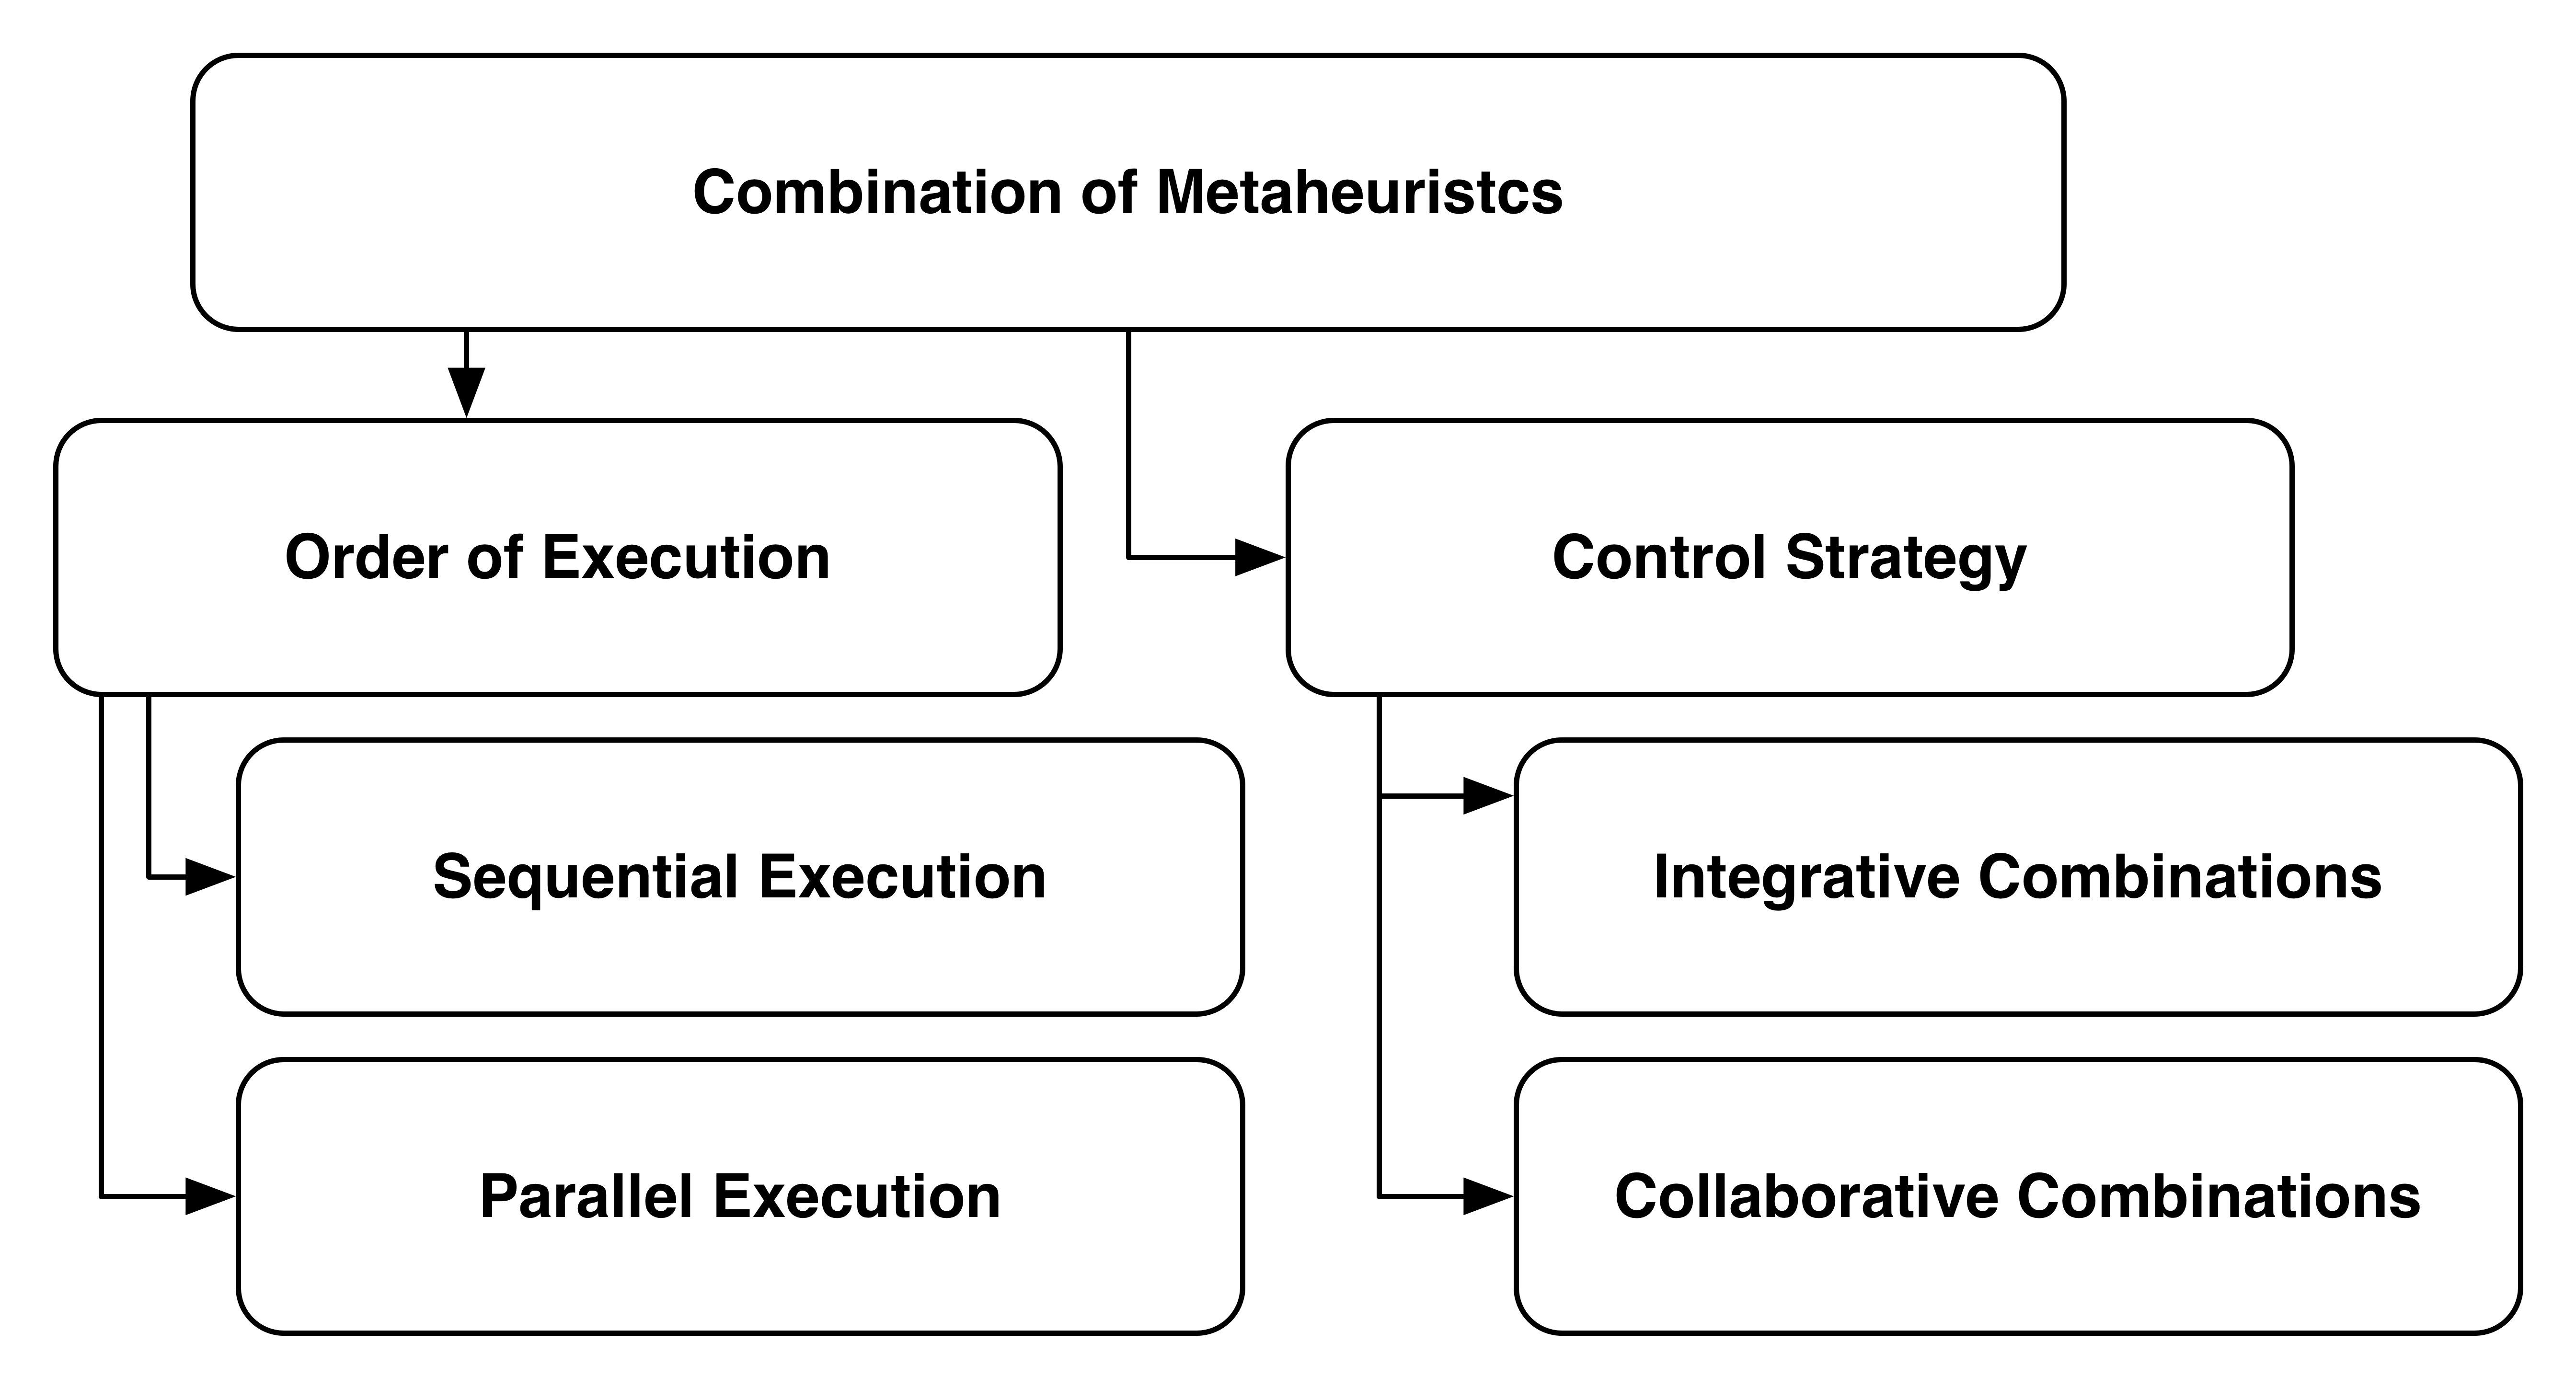
\includegraphics[width=0.8\textwidth]{./images/metaheuristc2.png}
\caption{Categories of metaheuristic combinations \cite{Puchinger2005} }
\label{fig:metaheuristc}
\end{figure}

Collaborative combinations use an approach where the algorithms exchange information, but are not part of each other. In this approach, algorithms may be executed sequentially or in parallel.

One of the most popular ways of metaheuristic hybridization consists in the use of trajectory methods inside population-based methods. Population-based methods are better in identifying promising areas of the search space from which trajectory methods can quickly reach good local optima. Therefore, metaheuristic hybrids that can effectively combine the strengths of both population-based methods and trajectory methods are often very successful \cite{raidl2010metaheuristic}.

\subsection{Multi-objective Metaheuristics}

Many real optimization problems require optimizing multiple conflicting objectives. There is no single optimal solution, but a set of alternative solutions. The objectives that have to be optimized are often in competition with one another and may be contradictory; we may find ourselves trying to balance the different optimization objectives of several distinct goals \cite{Harman2010}. The image of all the efficient solutions is called the Pareto front or Pareto curve or surface. The shape of the Pareto surface indicates the nature of the trade-off between the different objective functions. An example of a Pareto curve is reported in Fig. \ref{fig:pareto1}. Multi-objective optimization methods have as main purposes to minimize the distance between the nondominated front and the Pareto optimal front and find a set of solutions that are as diverse as possible.

\begin{figure}[h]
\centering
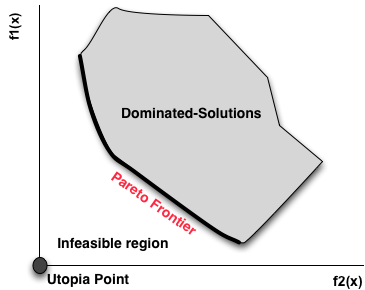
\includegraphics[width=0.4\textwidth]{./images/paretofront.png}
\caption{An optimized Pareto front example}
\label{fig:pareto1}
\end{figure}

What distinguishes multi-objective evolutionary algorithms from single objective metaheuristics is how they rank and select individuals in the population. If there is only one objective, individuals are naturally ranked according to this objective, and it is clear which individuals are best and should be selected as
parents. In the case of multiple objectives, it is still necessary to rank the individuals, but it is no longer obvious how doing this. Most people probably agree that a good approximation to the Pareto front is characterized by:

\begin{itemize}
\item  a small distance of the solutions to the true Pareto frontier,
\item  a wide range of solutions, i.e., an approximation
of the extreme values, and
\item a good distribution of solutions, i.e., an even
spread along the Pareto frontier.
\end{itemize}

The approximation of the Pareto-optimal set involves itself two objectives: minimize the distance to the optimal front and maximize the diversity of the generated solutions. There are two fundamental issues when designing a multiobjective evolutionary algorithm: mating selection and environmental selection. The first issue is related to the question of how to guide the search towards the Pareto-optimal front. The procedure to fill the mating pool is usually randomized. The second issue is related to the question of which individuals to keep during the evolution process. In most modern multi-objective algorithms these two concepts are realized in the following way: Environmental selection or Mating selection \cite{Zitzler2001}.

In  Environmental selection, an archive is maintained which contains a representation of the nondominated front among all solutions considered so far. A member of the archive is only removed if i) a solution has been found that dominates it or ii) the maximum archive size is exceeded and the portion of the front where the archive member is located is overcrowded \cite{Zitzler2001}.

In Mating selection, the pool of individuals is evaluated in two phases. First, all individuals are compared on the basis of the Pareto dominance. Basically, the information which individuals each individual dominates, is dominated by or is indifferent to is used to define a ranking on the generation pool. Afterwards, this ranking is refined by the incorporation of density information. Various density estimation techniques are used to measure the size of the niche in which a specific individual is located \cite{Zitzler2001}.


\subsubsection{NSGA-II Multi-objective Heuristics}

Multi-objective metaheuristics rank individuals according to the defined goals. Deb et al. proposed the Nondominated Sorting Genetic Algorithm II (NSGA-II) algorithm taking into account the need to reduce computational complexity in non-dominated classification while introducing elitism and eliminating subjectivity in the allocation of the sharing parameter \cite{Deb2000}. NSGA-II is a multi-objective algorithm, based on GAs, and implements the concept of dominance, in other words, to classify the total population in fronts according to the degree of dominance. According to NSGA-II, the individuals that are located on the first front are considered the best solutions of that generation, while in the last front are the worst. Using this concept, one can find more consistent results, located closer to the Pareto region, and better adapted to the type of problem.

The NSGA algorithm II applies a fitness evaluation in an initial population (Figure \ref{fig:nsga2}- \ding{202} and \ding{203}). The populations are ranked using multiple tournament selections, which consist of comparing two solutions (Figure \ref{fig:nsga2}- \ding{204}). In order to estimate the density of the solutions surrounding a particular solution in the population, the common distance between the previous solution and the posterior is calculated for each of the objectives. This distance serves as an estimate of the size of the largest cuboid that includes solution i without including any other solution of the population. A solution i beats another solution if:

\begin{itemize}
\item Solution i has a better rank, then $Rank_i$ <$Rank_j$.
\item Both solutions have the same rank, but i has a greater Distance than j, then $Rank_i$ = $Rank_j$ and $Distance_i$>$Distance_j$.
\end{itemize}

At the end of each analysis a certain group of individuals is classified as belonging to a specific category called the front, and upon completion of the classification process, all individuals will be inserted into one of the n fronts. Front 1 is made up of all nondominated solutions. Front 2 can be achieved by considering all nondominated solutions excluding solutions from front 1. For the determination of front 3, solutions previously classified on front 1 and 2 are excluded, and so on until all individuals have been classified on some front.

After selection, recombination and mutation are performed as in conventional GAs (Figure \ref{fig:nsga2}- \ding{205}). The two sets (father and son of the same dimension) are united in a single population (dimension 2) and the classification is applied in dominance fronts. In this way, elitism is guaranteed preserving the best solutions (fronts are not dominated) in the latest population (Figure \ref{fig:nsga2}- \ding{207}).

However, not all fronts can be included in the new population. Thus, Deb et al. proposed a method called crowd distance, which combines the fronts not included in the set, to compose of the last spaces of the current population, guaranteeing the diversity of the population \cite{Deb2000}. The NSGA-II algorithm creates a set of front lines, in which each front containing only non–dominating solutions. Within a front, individuals are rewarded for being ‘spread out’. The algorithm also ensures that the lowest ranked individual of a front still has a greater fitness value than the highest ranked individual of the next front \cite{Yoo2007}.




\begin{figure}[h]
\centering
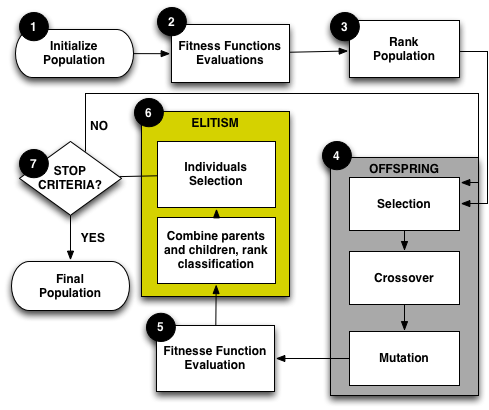
\includegraphics[width=0.5\textwidth]{./images/NSGA-2.png}
\caption{NSGA-II Algorithm}
\label{fig:nsga2}
\end{figure}

\subsubsection{SPEA2: Improving the Strength Pareto Evolutionary Algorithm}

SPEA uses a regular population and an archive. Starting with an initial population and an empty archive the following steps are performed per iteration. First, all non-dominated population members are copied to the archive; any dominated individuals or duplicates are removed. If the size of the updated archive exceeds a predefined limit, further archive members are deleted by a clustering technique which preserves the characteristics of the non-dominated front. Afterwards, fitness values are assigned to both archive and population members. Each individual i in the archive assign a strength value S(i) $\in$ [0, 1], which at the same time represents its fitness value F(i). 0 indicates a non-dominated individual,whereas a high value points out that the individual is dominated by many other ones. S(i) is the number of population members j that are dominated by or equal to i with respect to the objective values, divided by the population size plus one. The algorithmic framework of SPEA2 is described in Alg. \ref{spea2}. An initial population $P_{0}$ and an initial archive are created. The fitness value of all individuals is calculated in population and in the archive (external set). All non-dominated individual are copied to the new archive. Finally, the algorithm select the individual using a tournament selection \cite{Zitzler2001} \cite{Tervonen2017} \cite{MatneiFilho2016}.

\begin{algorithm}[h]
  \caption{SPEA2 Algorithm \cite{Zitzler2001}}\label{spea2}
  \begin{algorithmic}[1]

    \State Read N - Population size
    \State Read $ \overset{-}{N}$ - Archive size
    \State Read T - Maximum number of generations
    \State Generate a initial population $P_{0}$
    \State Create a initial archive $ \overset{-}{P} $
    \State Set T to zero
    \State Calculate the fitness value of individuals in $P_{t}$
    \State Calculate the fitness value of individuals in $\overset{-}{P}_{t}$
    \State Environmental Selection - Copy all non-dominated individuals in $P_{t}$ and $\overset{-}{P}_{t}$  to $\overset{-}{P}_{t+1}$
    \If {size of  $\overset{-}{P}_{t+1}$ exceeds  $ \overset{-}{N}$ }
    \State reduce  $\overset{-}{P}_{t+1}$ by means of truncation operator
    \ElsIf { size of  $\overset{-}{P}_{t+1}$ less than  $\overset{-}{N}$ }
    \State fill $\overset{-}{P}_{t+1}$ with dominated individuals in $P_{t}$ and $\overset{-}{P}_{t}$
    \EndIf
    \If {t $\gg$ T or another stopping criterion is satisfied }
    \State set A to the set of decision vectors represented by non-dominated individuals in $\overset{-}{P}_{t+1}$
    \State Stop
    \EndIf
    \State Mating selection - Perform binary tournament selection with replacement on $\overset{-}{P}_{t+1}$ in order to fill the mating pool
  \end{algorithmic}
\end{algorithm}

The main differences between SPEA2 and NSGA-II are the diversity assignment and replacement. NSGA-II uses a fast non-dominated sorting algorithm and uses Pareto optimal levels as the primary criterion to select solutions. SPEA2 derives the strength of each solution from the number of other solutions it dominates. NSGA-II uses the crowding-distance to maintain a well-spread set of solutions whereas SPEA2 applies the k-nearest neighbor approach (Figure \ref{fig:speansga}) \cite{Tervonen2017} \cite{Deb2005}.


\begin{figure}[h]
\begin{minipage}{.6\textwidth}
\centering
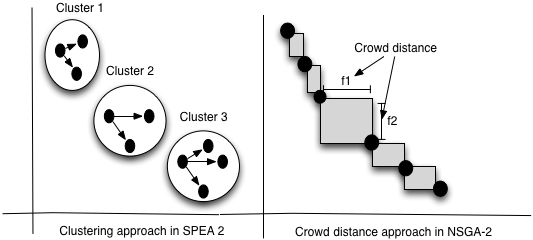
\includegraphics[width=1\textwidth]{./images/speansga.png}
\caption{Comparison between SPEA-2 and NSGA-II \cite{Deb2005}}
\label{fig:speansga}
\end{minipage}
\begin{minipage}{.4\textwidth}
\centering
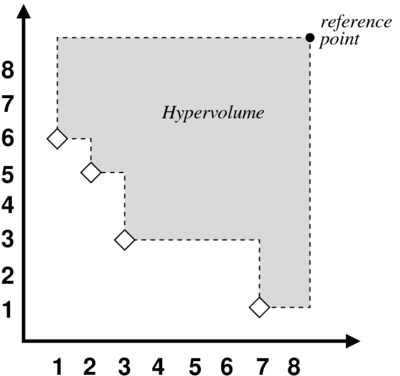
\includegraphics[width=0.7\textwidth]{./images/hypervolume-annot.png}
\caption{Hypervolume metric \cite{Lacour2015}}
\label{fig:hypervolume}
\end{minipage}
\end{figure}


\subsubsection{Pareto Archived Evolution Strategy} 

Pareto Archived Evolution Strategy(PAES) is an  evolutionary algorithm which employs
local search for the generation of new candidate solutions but
utilises population information in its selection procedure. The PAES algorithm was developed with two main objectives. The first of these was that the algorithm should be strictly confined to local search i.e. it should use a small change (mutation) operator only, and move from a current solution to a nearby neighbour. The second objective was that the algorithm should be a true Pareto optimiser, treating all non-dominated solutions as having equal value \cite{Knowles1999}. In PAES one parent generates by mutation one
offspring. The offspring is compared with the parent. If the offspring dominates the parent, the offspring is accepted as
the next parent and the iteration continues. If the parent dominates the offspring, the offspring is discarded and the new mutated solution (a new offspring) is generated. If the offspring and the parent do not dominate each other, a comparison set of previously non-dominated individuals is used \cite{Knowles1999}\cite{Oltean2005}. The algorithmic framework of PAES is described in Alg. \ref{paes}.


\begin{algorithm}[h]
  \caption{PAES Algorithm \cite{Knowles1999}\cite{Oltean2005}}\label{paes}
  \begin{algorithmic}[1]
    \State Repeat until a termination criterion has been reached
    \State Generate initial random solution c and add it to archive
    \State Mutate c to produce m and evaluate m
    \If {c dominates m }
    \State discard m
    \Else
    \If {m dominates c}
     \State replace c with m and add m to the archive
    \Else
    \If {m is dominated by any member of the archive}
    \State discard m
    \Else
    \State apply test (c, m, archive) to determine which becomes the new current solution and whether to add m to the archive
    \EndIf
    \EndIf
    \EndIf
  \end{algorithmic}
\end{algorithm}

\subsubsection{A Multiobjective Evolutionary Algorithm Based on Decomposition}

The Multiobjective Evolutionary Algorithm Based on Decomposition (MOEA/D) is a multiobjective evolutionary algorithm competitive to other well-known multiobjective optimization evolutionary algorithms (MOEAs) such as NSGA-II or SPEA-2 \cite{Michalak2014}. MOEA/D decomposes a multiobjective optimization problem into a number of scalar optimization subproblems and optimizes them simultaneously. Each subproblem is optimized by only using information from its several neighboring subproblems, which makes MOEA/D have lower computational complexity at each generation than MOGLS and non-dominated sorting genetic
algorithm II (NSGA-II) \cite{Zhang2007}. 

NSGA-II, SPEA2 and PAES algorithms  do not associate each individual solution with
any particular scalar optimization problem. In a scalar objective optimization problem, all the solutions can be compared based
on their objective function values and the task of a scalar objective evolutionary algorithm (EA) is often to find one single
optimal solution. MOEA/D explicitly decomposes the problem into scalar optimization subproblems.It solves these subproblems simultaneously by evolving
a population of solutions. At each generation, the population is
composed of the best solution found so far for each subproblem. The neighborhood relations among these subproblems are defined based on the distances between their aggregation coefficient vectors \cite{Zhang2007} \cite{McConaghy2011}. Fig. \ref{fig:moead} MOEA/D create a set of subproblems $W_{i}$. Each subproblem $W_{i}$ is improved to obtain the Pareto frontier \cite{McConaghy2011}. 


\begin{figure}[h]
\centering
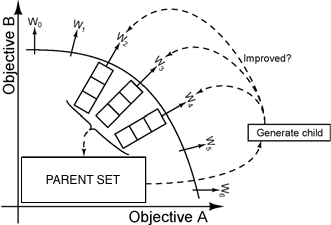
\includegraphics[width=0.5\textwidth]{./images/moead.png}
\caption{MOEA/D algorithm subproblems \cite{McConaghy2011}}
\label{fig:moead}
\end{figure}

The Alg. \ref{moead} presents the details of the algorithm. The algorithm  includes the
use of Tchebycheff approach as the decomposition method, with dynamical resource allocation, to improve the efficiency of the MOEA/D \cite{Yuen2009}. 

\begin{algorithm}[h]
  \caption{MOEA/D Algorithm}
  \label{moead}
  \begin{algorithmic}[1]
    \State \textbf{Initialization}
    \State Generate initial population by uniformly spreading and randomly sampling from search space
    \State Calculate the reference point for the Tchebycheff approach.
   \State Evaluate Objective Values 
   \State Selection using tournament selection method 
   \State Selection of mating and updating range
   \State Reproduction
   \State Repair
   \State Update of solutions 
   \State \textbf{Update}
   \State While (not equal to termination condition)
  \State Evaluate Objective Values
  \State Selection using tournament selection method
  \State Selection of mating and update range
  \State Reproduction
  \State Repair - if the searching element is out of boundary
  \State Update the solutions 
  \State \textbf{Stopping Criteria}
  \If {generation is a multiplication of a pre-set value of x}
  \State Update utility function;
  \EndIf    
  \end{algorithmic}
\end{algorithm}


\subsubsection{Comparing Multi-Objective Metaheuristics}

Deb states that are two orthogonal goals for any multi-objective algorithm \cite{deb2001multi}:

\begin{itemize}
\item Identify solutions as close as possible  to the true Pareto frontier;
\item identify a diverse of sets of solutions distributed across the entire Pareto-optimal surface.
\end{itemize}

There are several metrics either closeness or diversity. Example of metrics which measure the closeness of Pareto frontier is Error ratio and Set coverage. Example of metrics which measure the diversity are the Spacing and the Spread. The Hypervolume metric measure both closeness and diversity \cite{janssens2010multiple}. The Hypervolume metric calculates the volume in an objective space covered by the non-dominated individuals. The hypervolume was originally proposed by Zitzler and Thiele \cite{Zitzler1999}. It is especially useful when the true Pareto-optimal solution is unknown. For each solution, a hypercube is computed from a reference point and the solution as the diagonal corners of the hypercube ( Figure \ref{fig:hypervolume} ) \cite{janssens2010multiple}. The reference point is found by constructing a vector of worst objects fitness value.


%The equation of the hypervolume is:


%\begin{equation}
%Hypervolume =  volume (U^{|Q|}_{i=1}  v_{i}  )
%\end{equation}



\section{Reinforcement Learning}

Reinforcement learning (RL) refers to both a learning problem and a sub-field of machine learning. As a learning problem, it refers to learning to control a system so as to maximize some numerical value which represents a long-term objective. The basic idea of Reinforcement Learning is simply to capture the most important aspects of the real problem, facing a learning agent interacting with its environment to achieve a goal \cite{Sutton2012}. Reinforcement learning is learning what to do—how to map situations to actions—so as to maximize a numerical reward signal. The learner needs to discover which actions yield the most reward by trying them \cite{Sutton2012}. A typical setting where Reinforcement Learning operates is shown in Figure \ref{fig:agentenv}: A controller receives the controlled system’s state and a reward associated with the last state transition. It then calculates an action which is sent back to the system.

\begin{figure}
\centering
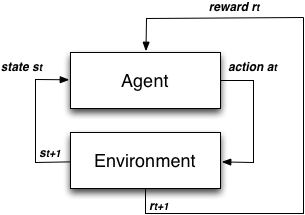
\includegraphics[width=0.4\textwidth]{./images/agentenv.png}
\caption{Example of interaction between some agent and the environment}
\label{fig:agentenv}
\end{figure}

In Reinforcement Learning, an agent wanders in an unknown environment and tries to maximize its long term return by performing actions and receiving rewards. The challenge is to understand how a current action will affect future rewards. A good way to model this task is with Markov Decision Processes (MDP). Markov decision processes (MDPs) provide a mathematical framework for modeling decision making. In Reinforcement Learning, all agents act in two phases: Exploration vs Exploitation. In Exploration phase, the agents try to discover better action selections to improve its knowledge. In Exploitation phase, the agents try to maximize its reward, based on what is already know.

One of the challenges that arise from reinforcement learning is the trade-off between exploration and exploitation. To obtain a large reward, a reinforcement learning
agent must prefer actions that it has tried in the past and found to be effective in producing reward. But to discover such actions, it has to try actions that it has not selected before. The agent has to exploit what it already knows in order to obtain a reward, but it also has to explore in order to make better action selections in the future. Q-learning is a model-free reinforcement learning technique. Q-learning is a multi-agent learning algorithm that learns equilibrium policies in Markov games, just as Q-learning learns to optimize policies in Markov decision processes \cite{Greenwald2003}. Q-learning and related algorithms try to learn the optimal policy from its history of interaction with the environment. A history of an agent is a sequence of state-action-rewards.Where $s_{n}$ is a state, $a_{n}$ is an action and $r_{n}$ is a reward:

\begin{equation}
<s_{0},a_{0},r_{1},s_{1},a_{1},r_{2},s_{2},a_{2},r_{3},s_{3},a_{3},r_{4},s_{4}....>,
\end{equation}


In Q-Learning, the system's objective is to learn a control policy $\pi = \sum_{n=0}^{\infty} \gamma\textsuperscript{n}  r_{t}+n $, where $\pi$  is the discounted cumulative reward, $\gamma$ is the discount rate ($01$) and $r_{t}$ is the reward received after  the execution of an action at time t. Figure \ref{fig:qalgo} shows the summary version of Q-Learning algorithm. The first step is to generate the initial state of the MDP. The second step is to choose the best action or a random action based on the reward, hence the actions with best rewards are chosen.

\begin{figure}[h]
\centering
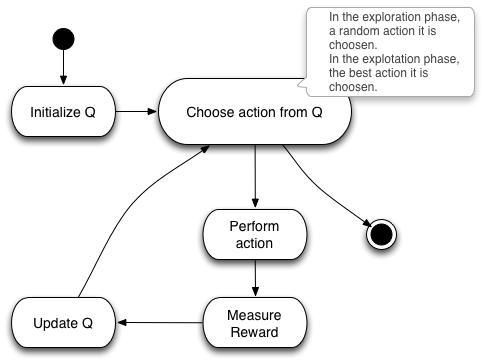
\includegraphics[width=0.6\textwidth]{./images/qalgo.png}
\caption{Q Learning algorithm}
\label{fig:qalgo}
\end{figure}

\section{Summary}

Metaheuristics are strategies that guide the search process to efficiently explore the search space in order to find optimal solutions. There are different ways to classify and describe metaheuristic algorithm. Algorithms working on single solutions are called trajectory methods. They all share the property of describing a trajectory in the search space during the search process. Population-based metaheuristics perform search processes which describe the evolution of a set of points in the search space. Trajectory methods are characterized by a trajectory in the search space. Two common trajectory methods are Simulated Annealing and Tabu Search. Population-based metaheuristics could be viewed as an iterative improvement in a population of solutions. First, the population is initialized. Then, a new population of solutions is generated. Finally, this new population is integrated into the current one using some selection procedures. The combination of one metaheuristic with components from other metaheuristics is called a hybrid metaheuristic. One of the most popular ways of metaheuristic hybridization consists in the use of trajectory methods inside population-based methods. Multi-objective optimization methods have as main purposes to minimize the distance between the non-dominated front and the Pareto optimal front and find a set of solutions that are as diverse as possible. Reinforcement learning is the problem of getting an agent to act in the unknown world so as to maximize its rewards. The next chapter presents the state-of-art of search-based stress testing.

\chapter{Search-based Stress Testing}

In this chapter, we introduce the context where this thesis is inserted and discuss the relevant state-of-the-art related to Search-based Stress Testing.

\section{Load, Performance and Stress Testing}

Load, performance, and stress testing are typically done to locate bottlenecks in a system, to support a performance-tuning effort, and to collect other performance-related indicators to help stakeholders get informed about the quality of the application being tested \cite{Sandler2004} \cite{Corporation2007}.

Typically, the most common kind of performance testing for Internet applications is load testing. Application load can be assessed in a variety of ways \cite{Perry2004}:

\begin{itemize}
\item Concurrency. Concurrency testing seeks to validate the performance of an application with a given number of concurrent interactive users \cite{Perry2004}.
\item Stress. Stress testing seeks to validate the performance of an application when certain aspects of the application are stretched to their maximum limits. This can include maximum number of users, and can also include maximizing table values and data values \cite{Perry2004}.
\item Throughput. Throughput testing seeks to validate the number of transactions to be processed by an application during a given period of time. For example, one type of throughput test might be to attempt to process 100,000 transactions in one hour \cite{Perry2004}.
\end{itemize}


Performance testing aims at verifying a specified system performance. This kind of test is executed by simulating hundreds of simultaneous users or more over a defined time interval \cite{DiLucca2006}. The purpose of this assessment is to demonstrate that the system reaches its performance objectives \cite{Sandler2004}.  Term often used interchangeably with “stress” and “load” testing. Ideally “performance” testing is defined in requirements documentation or QA or Test Plans \cite{Lewis2005}.


In a load testing, the system is evaluated at predefined load levels \cite{DiLucca2006}. The aim of this test is to determine whether the system can reach its performance targets for availability, concurrency, throughput, and response time. Load testing is the closest to real application use \cite{Molyneaux2009}. A typical load test can last from several hours to a few days, during which system behavior data like execution logs and various metrics are collected \cite{Afzal2009a}.

Stress testing investigates the behavior of the system under conditions
that overload its resources. The stress testing verifies the system behavior against heavy workloads \cite{Sandler2004} \cite{Lewis2005}, which are executed to evaluate a system beyond its limits, validate system response in activity peaks, and verify whether the system is able to recover from these conditions. It differs from other kinds of testing in that the system is executed on or beyond its breakpoints, forcing the application or the supporting infrastructure to fail \cite{DiLucca2006} \cite{Molyneaux2009}.

The main difference between load tests, performance tests and stress tests are:

\begin{itemize}

\item Performance tests demonstrate that the system reaches its performance objectives.
\item Load tests necessary use a load (concurrent or simultaneous users).
\item Stress tests differs from other kinds of testing in that the system is executed on or beyond its break-points, forcing the application or the supporting infrastructure to fail.
\end{itemize}


\section{Search-Based Testing}

Search-based software engineering (SBSE) is the application of optimization techniques in solving software engineering problems. The applicability of optimization techniques in solving software engineering problems is suitable as these problems frequently encountered competing constraints and require near optimal solutions \cite{Afzal2009a} \cite{Harman2015}.


Search-based Software Testing (SBST) is the subarea of Search Based Software Engineering concerned with software testing. Search-based software testing is the application of metaheuristic search techniques to generate software tests. The test adequacy criterion is transformed into a fitness function and a set of solutions in the search space are evaluated with respect to the fitness function using a metaheuristic search technique \cite{Afzal2009a} \cite{Aleti2016} \cite{Harman2015}. A variety of metaheuristic search techniques is found to be applicable for non-functional testing including simulated annealing, tabu search and genetic algorithms.

In the academic context, a number of studies proving the efficacy of metaheuristics to automate test execution can be found in the literature. Figure \ref{fig:sbsesbst}  shows the growth in papers published on SBST and SBSE. The data is taken from the SBSE repository (\url{http://crestweb.cs.ucl.ac.uk/resources/sbse_repository/}) and Afzal et al. \cite{Afzal2009a} \cite{Harman2015}.
The aim of the SBSE repository is to contain every SBSE paper. Although no repository can guarantee 100\% precision and recall, the SBSE repository has proved sufficiently usable that it has formed the basis of several other detailed analyses of the literature \cite{Harman2015}.


\begin{figure}[h]
\centering
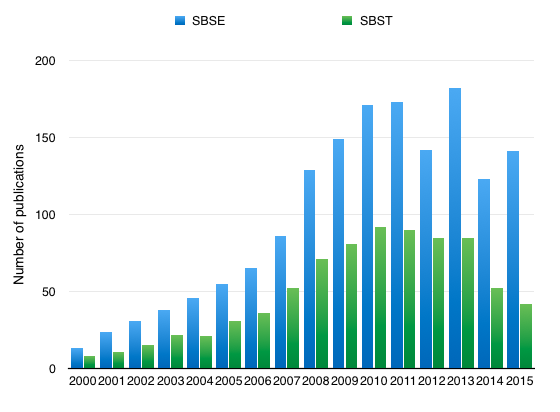
\includegraphics[width=0.7\textwidth]{./images/publications1.png}
\caption{Number of publications in SBSE and SBST by year \cite{Afzal2009a} \cite{Harman2015}}
\label{fig:sbsesbst}
\end{figure}

SBST has made many achievements and demonstrated its wide applicability and increasing uptake. Nevertheless, there are pressing open problems and challenges that need more attention like to extend SBST to test non-functional properties, a topic that remains relatively under-explored, compared to structural testing.  Fig. \ref{fig:nonfunctional} shows the non-functional SBST by year, data comes from the Harman et al., Afzal et al. and the SBSE repository \cite{Aleti2016} \cite{Harman2015}.


\begin{figure}[h]
\centering
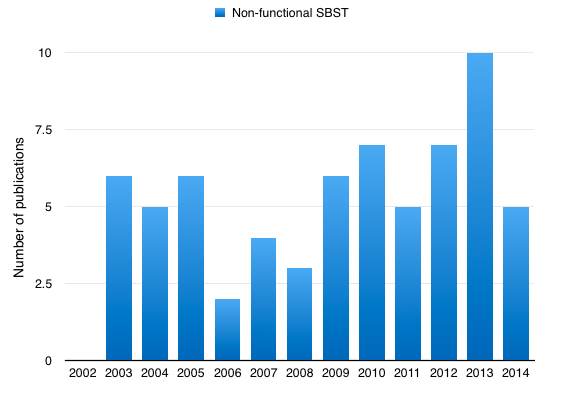
\includegraphics[width=0.6\textwidth]{./images/nonfunctional.png}
\caption{Number of publications in non-functional SBST by year \cite{Afzal2009a} \cite{Harman2015} }
\label{fig:nonfunctional}
\end{figure}



There are many kinds of non-functional search based tests  \cite{Afzal2009a}:

\begin{itemize}
\item Execution time: The application of evolutionary algorithms to find the best and worst case execution times (BCET, WCET).
\item Quality of service: uses metaheuristic search techniques to search violations of service level agreements (SLAs).
\item Security: apply a variety of metaheuristic search techniques to detect security vulnerabilities like detecting buffer overflows.
\item Usability: concerned with the construction of covering array which is a combinatorial object.
\item Safety: Safety testing is an important component of the testing strategy of safety critical systems where the systems are required to meet safety constraints.
\end{itemize}

A variety of metaheuristic search techniques is found to be applicable for non-functional testing including simulated annealing, tabu search, genetic algorithms, ant colony methods, grammatical evolution, genetic programming and swarm intelligence methods. However, most research studies are limited to making prototypes \cite{Afzal2009a}.  Fig. \ref{fig:metabykind} shows a comparison between the range of metaheuristics and the type of non-functional search based test.The Data comes from Afzal et al. \cite{Afzal2009a}. Afzal's work was added to some of the latest research in this area (\cite{Garousi2006} \cite{Garousi2010} \cite{DiAlesio2013} \cite{DiAlesio2014} \cite{Alesio2015} \cite{Gois2016}). The thesis focus is use  hybrid and multiobjective metaheuristics in Quality of Service and Execution Time tests (Search-based stress testing). There is a great difficulty in
comparing some approaches present in the state of
the art, due to the lack of availability of the tools used. The present research intends to compare the proposed approach with other methods based on the use of single or multiobjective metaheuristics. 


\begin{figure}[h]
\centering
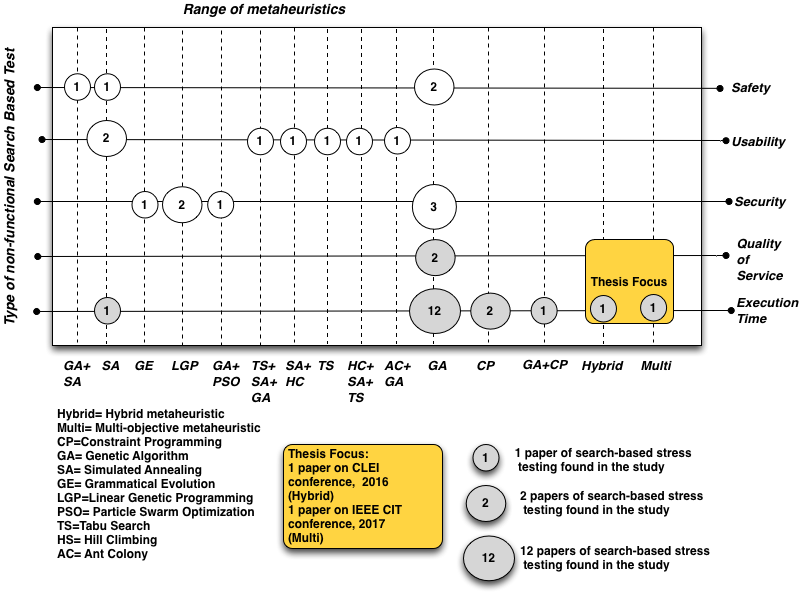
\includegraphics[width=1\textwidth]{./images/metaheuristics.png}
\caption{Range of metaheuristics by type of non-functional Search Based Test\cite{Afzal2009a}. }
\label{fig:metabykind}
\end{figure}


\section{Search-based Stress testing}

The search for the longest execution time is regarded as a discontinuous, nonlinear, optimization problem, with the input domain of the system under test as a search space \cite{Sullivan}.  The application of SBST algorithms to stress tests involves finding the best- and worst-case execution times (B/WCET) to determine whether timing constraints are fulfilled \cite{Afzal2009a}.

There are two measurement units normally associated with the fitness function in a stress test: processor cycles and execution time. The processor cycle approach describes a fitness function in terms of processor cycles. The execution time approach involves executing the application under test and measuring the execution time \cite{Afzal2009a} \cite{tracey2000search}. Processor cycles measurement is deterministic in the sense that it is independent of system load and results in the same execution times for the same set of input parameters. However, such a measurement is dependent on the compiler and optimizer used, therefore, the processor cycles differ from each platform. Execution time measurement is a non-deterministic approach, in which there is no guarantee of obtaining the same test inputs \cite{Afzal2009a}.  However, stress testing where testers have no access to the production environment should be measured by the execution time measurement \cite{Molyneaux2009} \cite{Afzal2009a}.

Table \ref{tab:comparison}  shows a comparison between the research studies on load, performance, and stress tests presented by Afzal et al. \cite{Afzal2009a}. Afzal's work was added with some of the latest research in this area (\cite{Garousi2006} \cite{Garousi2010} \cite{DiAlesio2013} \cite{DiAlesio2014} \cite{Alesio2015} \cite{Gois2016} ). The columns represent the type of tool used (prototype or functional tool), and the rows represent the metaheuristic approach used in each research study (genetic algorithm, Tabu search, simulated annealing, or a customized algorithm). The table also sorts the research studies by the type of fitness function used (execution time or processor cycles).


\begin{table}[!h]
\centering
\caption{Distribution of the research studies over the range of applied metaheuristics}
\label{tab:comparison}
\begin{tabular}{p{2.6cm}|p{4.8cm}|p{4.8cm}|p{3.8cm}|}
\cline{2-4}
                                                                & \multicolumn{2}{c|}{\textbf{Prototypes}}            & \textbf{Functional Tool} \\ \cline{2-4}
                                                                & \begin{minipage}{0.2\textwidth}\footnotesize Execution Time  \end{minipage}          & \begin{minipage}{0.2\textwidth}\footnotesize Processor Cycles \end{minipage}        & \begin{minipage}{0.2\textwidth}\footnotesize Execution Time \end{minipage}           \\ \cline{2-4}
%\setlength{\extrarowheight}{20pt}
\begin{tabular}[c]{@{}l@{}}\begin{minipage}{0.3\textwidth}\small GA + SA + \\ Tabu  Search\\ +Q-Learning \\ + Multi-objective \\ heuristics \\ NSGA-II, SPEA2\\ PAES,MOEA/D \\ \end{minipage}\end{tabular}  & \cellcolor[HTML]{FFFFFF} & \cellcolor[HTML]{FFFFFF} & \cellcolor[HTML]{FFFFFF} \begin{minipage}{0.2\textwidth}  \cellcolor{blue!25} \small Our approach \cite{Gois2016} \cite{Gois2017} \end{minipage}  \\[2ex] \cline{2-4}
\begin{minipage}{0.1\textwidth}\small GA \end{minipage}                                                              & \cellcolor[HTML]{FFFFFF} \begin{minipage}{0.3\textwidth}   \small \textnormal{ Alander et al.,1998 \\ \cite{Alander} \\ 
Wegener et al., 1996 and 1997 \\
\cite{Wegener1997} \\
\cite{J.WegenerK.GrimmM.GrochtmannH.Sthamer1996} \\
\cite{Sullivan} \\
\cite{Briand2005} \\ Canfora et al., 2005 \cite{Canfora}  \\ }\end{minipage} & \cellcolor[HTML]{FFFFFF} \begin{minipage}{0.3\textwidth} \small \textrm{  \\ Wegener and Grochtmann,\\ 1998 \cite{Wegener1998} \\  Mueller et al., 1998 \cite{Mueller1998} \\ Puschner et al. \cite{Puschner1998} \\ Wegener et al., 2000 \cite{Stations} \\ Gro et al., 2000 \cite{Gross2000}  \\ }\end{minipage}& \cellcolor[HTML]{FFFFFF} \begin{minipage}{0.22\textwidth}   \small \textnormal{ \\  Di Penta et al., 2007 \cite{Penta2007} \\ Garoussi, 2006 \cite{Garousi2006} \\ Garousi, 2008 \cite{Garousi2008} \\ Garousi, 2010 \cite{Garousi2010} \\ } \end{minipage} \\  \Cline{3pt}{2-4}
\begin{minipage}{0.1\textwidth}\small Simulated \\ Annealing \\ (SA) \end{minipage}                                                             & \cellcolor[HTML]{FFFFFF} & \cellcolor[HTML]{FFFFFF} & \cellcolor[HTML]{FFFFFF} \begin{minipage}{0.2\textwidth}   \small  Tracey, 1998 \\\cite{Tracey1998} \end{minipage} \\[2ex] \cline{2-4}
\begin{minipage}{0.1\textwidth}\small  Constraint \\ Programming \end{minipage}                                                             & \cellcolor[HTML]{FFFFFF} & \cellcolor[HTML]{FFFFFF} & \cellcolor[HTML]{FFFFFF} \begin{minipage}{0.3\textwidth}   \small  Di Alesio et al., 2014 \\ \cite{DiAlesio2014} \\ Di Alesio et al., 2013 \\ \cite{DiAlesio2013}  \end{minipage} \\[2ex] \cline{2-4}
\begin{minipage}{0.1\textwidth}\small  GA +\\ Constraint \\ Programming \end{minipage}                                                             & \cellcolor[HTML]{FFFFFF} & \cellcolor[HTML]{FFFFFF} & \cellcolor[HTML]{FFFFFF} \begin{minipage}{0.3\textwidth}   \small  Di Alesio et al., 2015 \\ \cite{Alesio2015} \end{minipage} \\[2ex] \cline{2-4}
\setlength{\extrarowheight}{20pt}
\begin{tabular}[c]{@{}l@{}}
\begin{minipage}{0.1\textwidth}\small Customized \\ Algorithm \end{minipage}\end{tabular} & \cellcolor[HTML]{FFFFFF} & \cellcolor[HTML]{FFFFFF}  \begin{minipage}{0.3\textwidth}   \small  \textnormal{   \raggedleft Pohlheim, 1999 \cite{Pohlheim2005}  } \end{minipage} & \cellcolor[HTML]{FFFFFF} \\[4ex] \cline{2-4}
\setlength{\extrarowheight}{20pt}
\begin{tabular}[c]{@{}l@{}}
\begin{minipage}{0.1\textwidth}\small SIBEA  \\  Multi-object \\ algorithm  \end{minipage}\end{tabular} & \cellcolor[HTML]{FFFFFF} \begin{minipage}{0.3\textwidth}   \small  \textnormal{\raggedleft Woehrle, 2012  \cite{Woehrle2012} } \end{minipage} & \cellcolor[HTML]{FFFFFF} & \cellcolor[HTML]{FFFFFF} \\[4ex] \cline{2-4}
\end{tabular}
\end{table}

The studies can be grouped into two main groups: Search-Based Stress Testing on Safety-critical systems or Search-Based Stress Testing on non Safety-critical systems.


\subsection{Search-Based Stress Testing on Safety-critical Systems}

Domains such as avionics, automotive and aerospace feature safety-critical systems, whose failure could result in catastrophic consequences.  The importance
of software in such systems is permanently increasing due to the need of a higher system
flexibility. For this reason, software components of these systems are usually subject to safety certification. In this context, software safety certification has to take into account performance requirements specifying constraints on how the system should react to its environment, and how it should execute on its hardware platform \cite{DiAlesio2013}.

Usually, embedded computer systems have to fulfill real-time requirements. A faultless function of the systems does not depend only on their logical correctness but also on their temporal correctness. Dynamic aspects like the duration of computations, the memory actually needed during program execution, and other synchronization of parallel processes are of major importance for the correct function of real-time systems  \cite{J.WegenerK.GrimmM.GrochtmannH.Sthamer1996} .

The concurrent nature of embedded software makes  the order of external events triggering the system tasks are often unpredictable. Such increasing software complexity
renders performance analysis and testing increasingly
challenging. This aspect is reflected by the fact that most existing testing approaches target system functionality rather than performance \cite{DiAlesio2013}. Reactive real-time systems must react to external events within time constraints. Triggered tasks must execute within deadlines. Shousha develops a methodology for the derivation of test cases that aims at maximizing the chance of critical deadline misses \cite{shousha2003performance}.

The main goal of Search-Based Stress testing of Safety-critical systems is finding a combination of inputs that cause the system to delay task completion to the greatest extent possible. The followed approaches use metaheuristics to discover the worst-case execution times. Wegener et al. \cite{Wegener1997} used GAs to search for input situations that produce very long or very short execution times. The fitness function used was the execution time of an individual measured in micro seconds \cite{Wegener1997}. Alander et al. \cite{Alander} performed experiments in a simulator environment to measure extreme response times of protection relay software using genetic algorithms. The fitness function used was the response time of the tested software. The results showed that GA generated more input cases with longer response times \cite{Alander}.

Wegener and Grochtmann performed an experiment to compare GA with random testing. The fitness function used was the execution duration measured in processor cycles.  The results showed that, with a large number of input parameters, GA obtained more extreme execution times with less or equal testing effort than random testing \cite{J.WegenerK.GrimmM.GrochtmannH.Sthamer1996} \cite{Wegener1998}. Gro et. al. \cite{Gross2000} presented a prediction model which can be used to predict evolutionary testability. The research confirmed that there is a relationship between the complexity of a test object and the ability of a search algorithm to produce input parameters according to B/WCET \cite{Gross2000}. Briand et al. \cite{Briand2005} used GA to find the sequence of arrival times of events for aperiodic tasks, which will cause the greatest delays in the execution of the target task. A prototype tool named real-time test tool (RTTT) was developed to facilitate the execution of runs of a GA. Two case studies were conducted and results illustrated that RTTT was a useful tool to stress a system under test \cite{Briand2005}.


Pohlheim and Wegener used an extension of genetic algorithms with multiple sub-populations, each using a different search strategy. The duration of execution, measured in processor cycles, was taken as the fitness
function. The GA found longer execution times for all the given modules in comparison with systematic testing \cite{Pohlheim2005}. Garousi presented a stress test methodology aimed at increasing the chances of discovering faults related to distributed traffic in distributed systems. The technique uses as input a specified UML 2.0 model of a system, augmented with timing information. The results indicate that the technique is significantly more effective at detecting distributed traffic-related faults when compared to standard test cases based on an operational profile \cite{Garousi2006}. Alesio, Nejati and Briand describe an approach based
on Constraint Programming (CP) to automate the generation of test cases that reveal, or are likely to, task deadline misses. They evaluate it through a comparison with a state-of-the-art approach based on GAs. In particular, the study compares CP and GA in five case studies for efficiency, effectiveness, and scalability. The experimental results show that, on the larger and more complex case studies, CP performs significantly better than GA. The research proposes a tool-supported, efficient and effective approach based on CP to generate stress test cases that maximize the likelihood of task deadline misses \cite{DiAlesio2013}.

Alesio describes stress test case generation as a search problem over the space of task arrival times. The research locates the worst-case scenarios maximizing deadline misses where each scenario characterizes a test case. The paper combines two strategies, GA and CP. The results show that, in comparison with GA and CP in isolation, GA+CP achieves nearly the same effectiveness as CP and the same efficiency and solution diversity as GA, thus combining the advantages of the two strategies. Alesio concludes that a combined GA+CP approach to stress testing is more likely to scale to large and complex systems \cite{Alesio2015}.

\subsection{Search-Based Stress Testing on non Safety-critical Systems}

Usually, the application of Search-Based Stress Testing on non safety-critical systems deals with the generation of test cases that cause Service Level Agreement (SLA) violations.


Tracey et al. \cite{Tracey1998} used simulated annealing (SA) to test four
simple programs. The results of the research presented that the use of SA was more effective with a larger parameter space. The authors highlighted the need for a detailed comparison of various optimization techniques to explore the worst-case execution time (WCET) and the best-case execution times (BCET) of the system under test \cite{Tracey1998}.

Di Penta et al. \cite{Penta2007} used GA to create test data that violated quality of service (QoS) constraints, causing SLA violations. The generated test data included combinations of inputs. The approach was applied to two case studies. The first case study was an audio processing workflow, and the second case study, a service producing charts \cite{Penta2007}.

Gois et al. propose a hybrid metaheuristic approach using genetic algorithms, simulated annealing, and tabu search algorithms to perform stress testing. A tool named IAdapter, a JMeter plugin used for performing search-based stress tests, was developed. Two experiments were performed to validate the solution. In the first experiment, the signed-rank Wilcoxon non-parametrical procedure was used for comparing the results. The significance level adopted was 0.05. The procedure showed that there was a significant improvement in the results with the Hybrid Metaheuristic approach.
In the second experiment, the whole process of stress and performance tests, which took 3 days and about 1800 executions, was carried out without the need for monitoring by a test designer. The tool automatically selected the next scenarios to be run up to the limit of the previously established six generations \cite{Gois2016}.

Gois et al. verify the use of a multi-objective algorithm in search-based stress testing. The NSGA-II algorithm was implemented in the IAdapter tool using the jMetal framework. The experiment uses the NSGA-II algorithm to discover application scenarios where there is a high response time for a small number of users.  The experiment found 9 optimal workloads that present a lower number of users with high response times \cite{Gois2017}.

\section{Similar approaches}

This research and Alesio's approach \cite{Alesio2015} use a hybrid approach with a functional tool in different contexts. Table \ref{tab:alesiogois} presents the main differences between Alesio's and this thesis's approaches. Whereas the present research uses an approach based on usage scenarios performing tests on an application installed in an available environment, Alesio uses sequence diagrams  to select for the arrival time of tasks in systems from  safety-critical domains. 


\begin{table}[h]
\centering
\caption{Main differences between Alesio's \cite{Alesio2015} and IAdapter's approaches}
\label{tab:alesiogois}
\begin{tabular}{l|l|l|}
\cline{2-3}
                                                                                  & Alesio et al. \cite{Alesio2015}                                                                                                             & This thesis                                                                                                                            \\ \hline
\multicolumn{1}{|l|}{Metaheuristcs}                                               & \begin{tabular}[c]{@{}l@{}}GA+ \\ Constraint Programming\end{tabular}                                                      & \begin{tabular}[c]{@{}l@{}}GA+SA+\\ Tabu Search\end{tabular}                                                                           \\ \hline
\multicolumn{1}{|l|}{Inputs}                                                      & \begin{tabular}[c]{@{}l@{}}Design Model (Time and \\ Concurrency\\  Information)\end{tabular}                              & \begin{tabular}[c]{@{}l@{}}Number of Users\\ and\ Test scenarios\end{tabular}                                                     \\ \hline
\multicolumn{1}{|l|}{\begin{tabular}[c]{@{}l@{}}Main\\ Objective\end{tabular}}    & \begin{tabular}[c]{@{}l@{}}Find task arrival times\\ of aperiodic tasks that\\  maximizing\\  deadline misses\end{tabular} & \begin{tabular}[c]{@{}l@{}}Find the number of\\  users and \\ test scenarios that\\ maximizing\\ the response time\end{tabular} \\ \hline
\multicolumn{1}{|l|}{\begin{tabular}[c]{@{}l@{}}Main \\ Application\end{tabular}} & \begin{tabular}[c]{@{}l@{}}Systems from \\ safety-critical \\ domains\end{tabular}                                         & \begin{tabular}[c]{@{}l@{}}Web and Mobile \\ applications\end{tabular}                                                                 \\ \hline
\end{tabular}
\end{table}

Woehrle and this thesis use multi-objective algorithms to stress testing in different contexts. Woehrle formulate stress testing of protocol stacks on specific topologies as a multi-objective optimization problem and use an evolutionary algorithm for finding a set of small topologies that particularly stress the protocol stack of a wireless network \cite{Woehrle2012}. 


\section{Summary}

The stress testing verifies the system behavior against heavy workloads, which are executed to evaluate a system beyond its limits, validate system response in activity peaks, and verify whether the system is able to recover from these conditions. Search-based software engineering (SBSE) is the application of optimization techniques in solving software engineering problems. The applicability of optimization techniques in solving software engineering problems is suitable as these problems frequently encounter competing constraints and require near optimal solutions.  Search-based software testing is the application of metaheuristic search techniques to generate software tests. The test adequacy criterion is transformed into a fitness function and a set of solutions in the search space is evaluated with respect to the fitness function using a metaheuristic search technique.

SBST has made many achievements and demonstrated its wide applicability and increasing uptake. Nevertheless, there are pressing open problems and challenges that need more attention like to extend SBST to test non-functional properties. A variety of metaheuristic search techniques is found to be applicable for non-functional testing including simulated annealing, tabu search, genetic algorithms, ant colony methods, grammatical evolution, genetic programming and swarm intelligence methods. However, most research studies are limited to making prototypes. The search for the longest execution time is regarded as a discontinuous, nonlinear, optimization problem, with the input domain of the system under test as a search space.  The application of SBST algorithms to  stress tests involves finding the best- and worst-case execution times (B/WCET) to determine whether timing constraints are fulfilled. There are two measurement units normally associated with the fitness function in a stress test: processor cycles and execution time. The processor cycle approach describes a fitness function in terms of processor cycles. The execution time approach involves executing the application under test and measuring the execution time. Processor cycles measurement is deterministic in the sense that it is independent of system load and results in the same execution times for the same set of input parameters.

The studies can be divided into two main groups: Search-Based Stress Testing on Safety-critical systems or Search-Based Stress Testing on non Safety-critical systems. Domains such as avionics feature safety-critical systems, whose failure could lead to catastrophic consequences.  The importance of software in such systems is permanently increasing due to the need of a higher system
flexibility. For this reason, software components of these systems are usually subject to safety certification. 

Usually, the application of Search-Based Stress Testing on non safety-critical systems deals with the generation of test cases that cause Service Level Agreement (SLA) violations. Tracey et al.  used simulated annealing (SA) to test four
simple programs. The results of the research presented that the use of SA was more effective with a larger parameter space. Di Penta et al. used GA to create test data that violated quality of service (QoS) constraints, causing SLA violations. The approach was applied to two case studies. The first case study was an audio processing workflow, and the second case study, a service producing charts. The next chapter presents the first contribution of this thesis.

\chapter{Stress Search Based Testing using Hybrid Metaheuristic}

This chapter presents a study of the use a hybrid algorithm in search-based stress testing. The research uses genetic algorithms, tabu search, and simulated annealing in two different approaches. The study initially investigated the use of these three algorithms independently. Subsequently, the study will focus on uses the three algorithms collaboratively (hybrid metaheuristic approach).

In the first approach, the algorithms do not share their best individuals among themselves. Each algorithm evolves in a separate way (Fig. \ref{fig:firstaproach}). The second approach uses the algorithms in a collaborative mode (hybrid metaheuristic). In this approach, the three algorithms share their best individuals found (Fig. \ref{fig:secondapproach}). 


The chapter also presents three experiments. The first experiment aimed to perform performance, load, and stress testing on a simulated component.The second experiment was performed with a Moodle application. The third experiment carried out to verify the best case scenarios found by the hybrid metaheuristic approach.  The next subsections present details about the used metaheuristic algorithms (Representation, initial population and fitness function).

\begin{figure}[h]
\centering
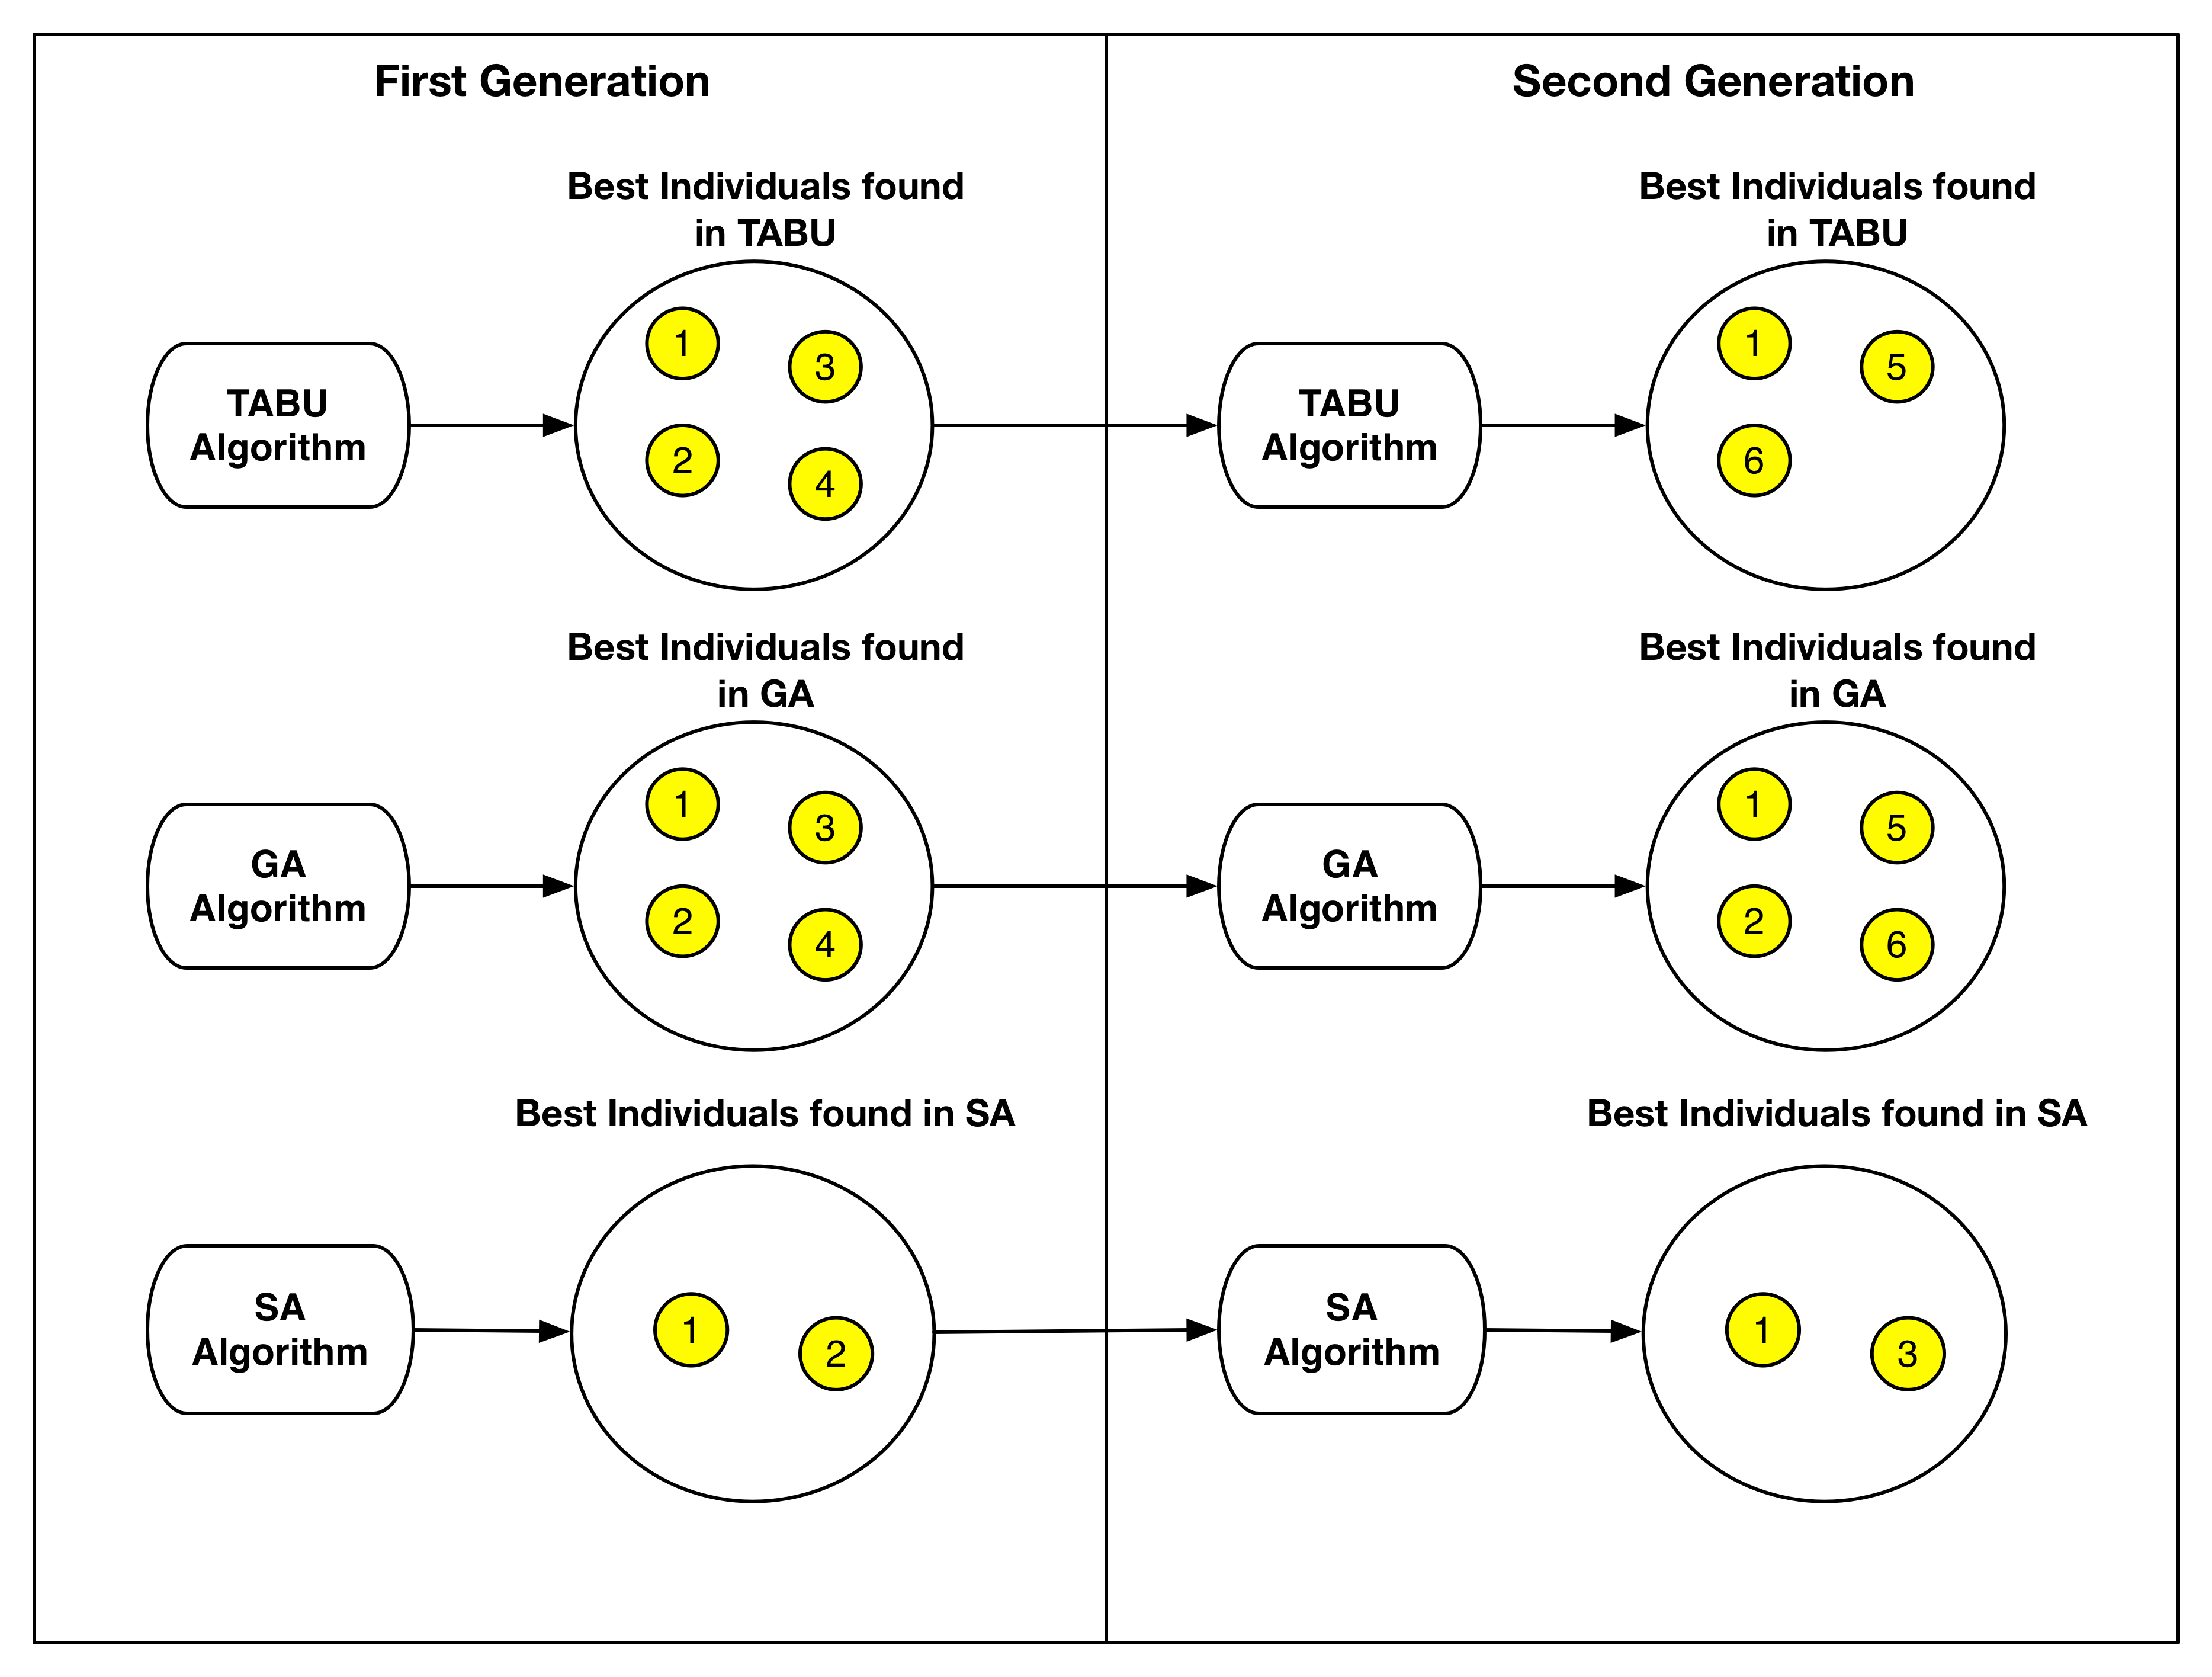
\includegraphics[width=0.7\textwidth]{./images/independ.png}
\caption{Use of the algorithms independently \cite{Gois2016}}
\label{fig:firstaproach}
\end{figure}

\begin{figure}[h]
\centering
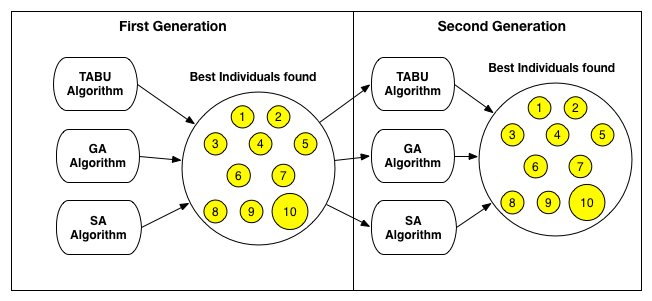
\includegraphics[width=0.7\textwidth]{./images/collaborative.png}
\caption{Use of the  algorithms collaboratively \cite{Gois2016}}
\label{fig:secondapproach}
\end{figure}



\section{Representation}

The solution representation provides a common representation for all workloads. Each workload is composed by a linear vector with 21 positions (Figure \ref{fig:solution}  -\ding{202}). The first position represents a metadata with the name of an individual. The next positions represent 10 scenarios and their numbers of users (Figure \ref{fig:solution}  -\ding{203}). The fixed-length genome approach was chosen in reason of the ease of implementation in the JMeter tool. Each scenario is an atomic operation: the scenario must log into the application, run the task goal, and undo any changes performed, returning the application to its original state.

Figure. \ref{fig:solution} presents the solution representation and an example using the crossover operation. In the example, solution 1 (Figure \ref{fig:solution}  -\ding{204}) has the Login scenario with 2 users, the Search scenario with 4 users, Include scenario with 1 user and the Delete scenario with 2 users.  After the crossover operation with solution 2 (Figure \ref{fig:solution}  -\ding{205}), We obtain a solution with the Login scenario with 2 users, the Search scenario with 4 users, the Update scenario with 3 users and the Include scenario with 5 users (Figure \ref{fig:solution}  -\ding{206}). Figure. \ref{fig:solution} -\ding{207} shows the strategy used by the proposed solution to  obtain the neighbors for the Tabu search and simulated annealing algorithms. The neighbors are obtained by the modification of a single position (scenario or number of users) in the vector.

\begin{figure}[h]
\centering
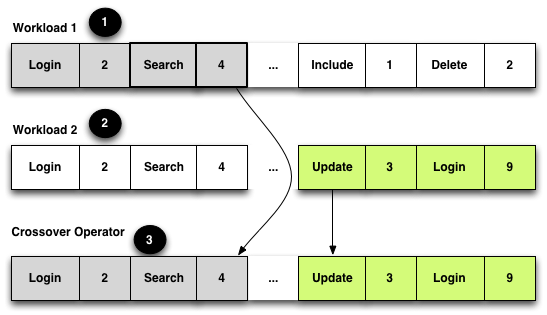
\includegraphics[width=0.7\textwidth]{./images/genomere.png}
\caption{Solution representation, crossover  and neighborhood operators \cite{Gois2016}}
\label{fig:solution}
\end{figure}

\section{Initial population}

The strategy used by the plugin to instantiate the initial population is to generate 50\% of the individuals randomly, and 50\% of the initial population is distributed in three ranges of values:

\begin{itemize}
\item Thirty percent of the maximum allowed users in the test;
\item Sixty percent of the maximum allowed users in the test; and
\item Ninety percent of the maximum allowed users in the test.
\end{itemize}

The percentages relate to the distribution of the users in the initial test scenarios of the solution. For example, in a hypothetical test with 100 users, the solution will create initial test scenarios with 30, 60 and 90 users.

\section{Objective (fitness) Function}

The proposed solution was designed to be used with independent testing teams in various situations, in which the teams have no direct access to the environment, where the application under test was installed. Therefore, the IAdapter plugin uses a measurement approach as the definition of the fitness function. The fitness function applied to the IAdapter solution is governed by the following equation:

\begin{equation}
\begin{aligned}
fit=numberOfUsersWeight*numberOfUsers\\
-90percentileweight* 90percentiletime\\
-80percentileweight*80percentiletime\\
-70percentileweight*70percentiletime\\
-maxResponseWeight*maxResponseTime\\
-penalty
\end{aligned}
\end{equation}

The users and response time factors were chosen because they are common units of measurement in load test tools \cite{Sandler2004}. The proposed solution's fitness function uses a series of manually adjustable user-defined weights (90percentileweight, 80percentileweight,  70percentileweight, maxResponseWeight, and numberOfUsersWeight). These weights make it possible to customize the search plugin's functionality. A penalty is applied when the response time of an application under test runs longer than the service level. The penalty is calculated by the following equation:

\begin{equation}
\begin{aligned}
penalty=100 * \Delta \\
\Delta=(t_{Current Response Time} - t_{Maximum Response Time Expected})\\
\end{aligned}
\end{equation}

\section{Experiments with Hybrid Algorithm}

This section presents three experiments. The first one was performed on an emulated component, the second one was performed using an installed Moodle application and the third one was performed using four antipatterns. The experiments used the following fitness function:

\begin{equation}
\begin{aligned}
fit=0.9* 90percentiletime\\
+0.1*80percentiletime\\+
0.1*70percentiletime+\\
0.1*maxResponseTime+\\
0.2*numberOfUsers-penalty
\end{aligned}
\end{equation}

This fitness function has manually adjustable user-defined weights filled out. This fitness function intended to find individuals with the highest percentile of 90\%, followed by individuals with a higher percentile time of 80\% and 70\%, maximum response time, and a number of users.

The first experiment ran for 27 generations, and the second experiment  performed 6 generations, with 300 executions by generation (100 times for each algorithm),  generating 300 new individuals. The experiments used an initial population of 100 individuals. The genetic algorithm used the top 10 individuals from each generation in the crossover operation. The Tabu list was configured with the size of 10 individuals and expired every 2 generations.  The mutation operation was applied to 10\% of the population on each generation.

\subsection{First Experiment: Emulated Class Test}

The first experiment aimed to perform performance, load, and stress testing on a simulated component. The purpose of using a simulated component was to be able to perform a greater number of generations in a shorter time available and eliminate variables such as the use of databases and application servers. The first experiment used a test class  named SimulateConcurrentAccess. This class has a static variable named \textit{x} and a set of methods that use the variable in a synchronized context ( Listing \ref{classsimulated}). The experiment was executed using the JMeter Java Request Sampler Component with IAdapter.

\lstdefinestyle{outline}{
		language=Java,
         basicstyle=\scriptsize\ttfamily,
         numberstyle=\tiny,
         numbersep=5pt,
         tabsize=2,
         extendedchars=true,
         breaklines=true,
         keywordstyle=\color{black}\bf,
         frame=b,  % <<<<<<<<<<<<<<<<<<<<<<<<<<
         stringstyle=\color{green!40!black}\ttfamily,
         showspaces=false,
         showtabs=false,
         numbers=left,
         xleftmargin=17pt,
         framexleftmargin=17pt,
         framextopmargin=1pt, % <<<<<<<<<<<<<<<<<<<<<<
         showstringspaces=false,
         %backgroundcolor=\color[RGB]{200,200,200},
         belowcaptionskip=0pt
}

\begin{lstlisting}[style=outline,caption={SimulateConcurrentAccess class},float,label=classsimulated]
public class SimulateConcurrentAccess {
  @Test
  public void firstScenario() {
    synchronized (StaticClass.class) {
			for (int i = 0; i <= 1000; i++) {
				StaticClass.x += i;
			}
			StaticClass.x = 0;
		}
	}

	  @Test
  public void secondScenario() {
    synchronized (StaticClass.class) {
			for (int i = 0; i <= 2000; i++) {
				StaticClass.x += i;
			}
			StaticClass.x = 0;
		}
	}
\end{lstlisting}


Fig.\ref{fig:exp1bestresults} presents the best results in 27 generations applied in the first experiment. The figure shows the results obtained with the algorithms with and without collaboration. The $x$ axis  represents the generation number, and the $y$ axis represents the best fitness value obtained until the current generation.
A higher value in the figure means that the scenario has a greater response time by the application under test. The results of the experiment showed that the use of cooperation between the three algorithms resulted in finding the individuals with better fitness values.

\begin{figure}[h]
\centering
\caption{Best results obtained in 27 generations}
\includegraphics[width=1\textwidth]{./images/generationcomparative.png}
\label{fig:exp1bestresults}
\end{figure}

Table \ref{tab:averagefirst} presents the results obtained by the hybrid metaheuristic (HM) approach, genetic algorithm (GA), simulated annealing (SA), and Tabu search (TS) from 27 generations in the first experiment. The values are the maximum fitness value obtained by each algorithm.

\begin{table}[h]
\centering
\caption{Maximum value of the fitness function by algorithm}
\label{tab:averagefirst}
\begin{tabular}{|l|l|l|l|l|}
\hline
GEN & HM & TS  & GA    & SA    \\ \hline
1          & 11238 & 11238         & 11238 & 11238 \\ \hline
2          & 11804 & 11596         & 11801 & 10677 \\ \hline
3          & 11787 & 8932          & 8411  & 10869 \\ \hline
4          & 11723 & 9753          & 9611  & 10760 \\ \hline
5          & 8164  & 9780          & 10738 & 4794  \\ \hline
6          & 11802 & 9781          & 11086 & 6120  \\ \hline
7          & 9985  & 5782          & 11272 & 11798 \\ \hline
8          & 11803 & 11749         & 10084 & 11309 \\ \hline
9          & 11806 & 7284          & 11633 & 10766 \\ \hline
10         & 11807 & 9386          & 11717 & 4557  \\ \hline
11         & 11802 & 9653          & 11802 & 11151 \\ \hline
12         & 11807 & 10594         & 11793 & 9434  \\ \hline
13         & 11802 & 10848         & 10382 & 11805 \\ \hline
14         & 11801 & 11551         & 7219  & 10237 \\ \hline
15         & 11807 & 1701          & 7189  & 9338  \\ \hline
16         & 11813 & 6203          & 11758 & 5321  \\ \hline
17         & 11805 & 10720         & 10805 & 11748 \\ \hline
18         & 9600  & 6371          & 11698 & 7818  \\ \hline
19         & 11733 & 8160          & 11648 & 11509 \\ \hline
20         & 9589  & 9428          & 11805 & 4813  \\ \hline
21         & 11800 & 9463          & 11798 & 10801 \\ \hline
22         & 11805 & 11799         & 11804 & 6029  \\ \hline
23         & 11836 & 11655         & 11800 & 3579  \\ \hline
24         & 11805 & 11512         & 11803 & 5761  \\ \hline
25         & 11804 & 11573         & 11802 & 9680  \\ \hline
26         & 11800 & 11575         & 11403 & 9388  \\ \hline
27         & 11805 & 10691         & 11745 & 9465  \\ \hline
\end{tabular}
\end{table}

The signed-rank Wilcoxon non-parametrical procedure was used for comparing the results with Z-value and W-value. The significant level adopted was 0.05. The Z-value obtained was -2.2736 and the p-value was 0.0232. The W-value obtained was 78. The critical value of W for N = 25 at p<= 0.05 was 89.The result was significant at p<= 0.05. The procedure showed that there was a significant improvement in the results with the collaborative approach.

\subsection{Second Experiment: Moodle Application Test}

The second experiment used a Moodle application installed on a machine with 500 GB of hard disk space and 8 GB of memory. The study used six application scenarios:

\begin{itemize}
\item PostDeleteMessage: This scenario posts and deletes messages in the Moodle application.
\item MyHome: This scenario accesses the homepage of the user's application.
\item Login: This scenario is responsible for user authentication by the application.
\item Notifications: This scenario involves entering the notification page of each user.
\item Start Page: This scenario shows the initial start page of the application.
\item Badge: This scenario involves entering the badge page.
\end{itemize}

The maximum tolerated response time in the test was 30 seconds.  Any  individuals who obtained a time longer than the stipulated maximum time suffered penalties.  The whole process of stress and performance tests, which took 3 days and about 1800 executions, was carried out without the need for monitoring by a test designer. The tool automatically selected the next scenarios to be run up to the limit of six generations previously established.

Table \ref{tab:secondexperiment} presents the maximum fitness value obtained by the hybrid metaheuristic (HM) approach, genetic algorithm (GA), simulated annealing (SA), and Tabu search (TS) in each generation.


\begin{table}[!h]
\centering
\caption{Results obtained from the second experiment}
\label{tab:secondexperiment}
\begin{tabular}{|l|l|l|l|l|}
\hline
GEN & HM    & TS    & GA    & SA    \\
\hline
1          & 32242 & 32242 & 32242 & 32242 \\
\hline
2          & 34599 & 32443 & 26290 & 35635 \\
\hline
3          & 35800 & 34896 & 34584 & 34248 \\
\hline
4          & 35782 & 34912 & 32689 & 25753 \\
\hline
5          & 35611 & 31833 & 34631 & 8366  \\
\hline
6          & 35362 & 35041 & 33397 & 9706 \\
\hline
\end{tabular}
\end{table}


The small number of samples of the experiment is insufficient to give a statistical significance to the results of the Wilcoxon procedure. However, it is noted that, in four of six generations, the collaborative approach presented the best values. The experiment succeeded in finding 29 individuals whose maximum time expected by the application was obtained.  Table \ref{tab:secondexperiment1} shows an example of the six individuals with the highest fitness values in the second experiment. The table shows the fitness value (Fit);  the name of the scenario (Scenario); the number of users (Users); and the percentiles of 90\%, 80\%, and 70\% (90per, 80per and 70per) in seconds.

% Please add the following required packages to your document preamble:
% \usepackage{multirow}
\begin{table}[!h]
\centering
\caption{Example of individuals obtained in the second experiment}
\label{tab:secondexperiment1}
\begin{tabular}{|p{0.2cm}|l|l|l|p{0.60cm}|p{0.60cm}|p{0.60cm}|}
\hline
Id&Fit&Scenario&Users&90per&80per&70per\\ \hline
\multirow{2}{*}{1} & \multirow{2}{*}{35800} & MyHome        & 31              & \multirow{2}{*}{30} & \multirow{2}{*}{29} & \multirow{2}{*}{10} \\ \cline{3-4}
                   &                        & Badges        & 4               &                     &                     &                     \\ \hline
\multirow{3}{*}{2} & \multirow{3}{*}{35795} & MyHome        & 30              & \multirow{3}{*}{30} & \multirow{3}{*}{29} & \multirow{3}{*}{10} \\ \cline{3-4}
                   &                        & Notifications & 2               &                     &                     &                     \\ \cline{3-4}
                   &                        & Badges        & 2               &                     &                     &                     \\ \hline
\multirow{2}{*}{3} & \multirow{2}{*}{35782} & MyHome        & 32              & \multirow{2}{*}{30} & \multirow{2}{*}{29} & \multirow{2}{*}{10} \\ \cline{3-4}
                   &                        & Badges        & 3               &                     &                     &                     \\ \hline
\multirow{3}{*}{4} & \multirow{3}{*}{35773} & MyHome        & 22              & \multirow{3}{*}{30} & \multirow{3}{*}{29} & \multirow{3}{*}{10} \\ \cline{3-4}
                   &                        & Notifications & 6               &                     &                     &                     \\ \cline{3-4}
                   &                        & Badges        & 9               &                     &                     &                     \\ \hline
\multirow{2}{*}{5} & \multirow{2}{*}{35771} & MyHome        & 28              & \multirow{2}{*}{30} & \multirow{2}{*}{29} & \multirow{2}{*}{9}  \\ \cline{3-4}
                   &                        & Badges        & 6               &                     &                     &                     \\ \hline
\multirow{2}{*}{6} & \multirow{2}{*}{35683} & MyHome        & 27              & \multirow{2}{*}{30} & \multirow{2}{*}{29} & \multirow{2}{*}{8}  \\ \cline{3-4}
                   &                        & Badges        & 10              &                     &                     &                     \\ \hline
\end{tabular}
\end{table}


Table \ref{fig:gened} presents the percentage of genes in all test scenarios by generation with and without collaboration. Most of the genes converged to the MyHome feature, which had the highest application response time.


% Please add the following required packages to your document preamble:
% \usepackage[table,xcdraw]{xcolor}
% If you use beamer only pass "xcolor=table" option, i.e. \documentclass[xcolor=table]{beamer}
\begin{table}[!h]
\centering
\caption{Percentage of genes in each scenario by generation }
\label{fig:gened}
\begin{tabular}{c|c|c|c|c|c|c|c|}
\hline
\rowcolor[HTML]{D3D3D3}
\multicolumn{1}{|c|}{\cellcolor[HTML]{FFFFFF}\textbf{Gen/}}   & \multicolumn{7}{c|}{\cellcolor[HTML]{D3D3D3}\textbf{Non collaboration approach}}                                                                                                                                                       \\ \cline{2-8}
\multicolumn{1}{|c|}{\textbf{Scenarios}}                      & \cellcolor[HTML]{F8FF00}Initial & \cellcolor[HTML]{F8FF00}1 & \cellcolor[HTML]{F8FF00}2 & \cellcolor[HTML]{F8FF00}3 & \cellcolor[HTML]{F8FF00}4 & \cellcolor[HTML]{F8FF00}5 & \cellcolor[HTML]{F8FF00}6                                \\ \hline
\multicolumn{1}{|c|}{\cellcolor[HTML]{D3D3D3}Badges}          & 20                              & 18                        & 16                        & 24                        & 15                        & 16                        & 17                                                       \\ \hline
\rowcolor[HTML]{F8FF00}
\multicolumn{1}{|c|}{\cellcolor[HTML]{F8FF00}\textbf{MyHome}} & \textbf{15}                     & \textbf{59}               & \textbf{55}               & \textbf{48}               & \textbf{53}               & \textbf{50}               & \multicolumn{1}{l|}{\cellcolor[HTML]{F8FF00}\textbf{52}} \\ \hline
\multicolumn{1}{|c|}{\cellcolor[HTML]{D3D3D3}StartPage}       & 15                              & 10                        & 12                        & 11                        & 20                        & 18                        & \multicolumn{1}{l|}{19}                                  \\ \hline
\multicolumn{1}{|c|}{\cellcolor[HTML]{D3D3D3}Notifications}   & 25                              & 5                         & 11                        & 10                        & 9                         & 10                        & \multicolumn{1}{l|}{9}                                   \\ \hline
\multicolumn{1}{|c|}{\cellcolor[HTML]{D3D3D3}Post}            & 8                               & 3                         & 1                         & 3                         & 1                         & 2                         & \multicolumn{1}{l|}{1}                                   \\ \hline
\multicolumn{1}{|c|}{\cellcolor[HTML]{D3D3D3}Login}           & 17                              & 5                         & 5                         & 4                         & 2                         & 4                         & \multicolumn{1}{l|}{2}                                   \\ \hline
\multicolumn{1}{l|}{}                                         & \multicolumn{7}{c|}{\cellcolor[HTML]{D3D3D3}\textbf{Collaboration approach}}                                                                                                                                                           \\ \hline
\multicolumn{1}{|c|}{\cellcolor[HTML]{D3D3D3}Badges}          & 20                              & 29                        & 16                        & 25                        & 9                         & 16                        & 9                                                        \\ \hline
\rowcolor[HTML]{F8FF00}
\multicolumn{1}{|c|}{\cellcolor[HTML]{F8FF00}\textbf{MyHome}} & \textbf{15}                     & \textbf{29}               & \textbf{69}               & \textbf{49}               & \textbf{74}               & \textbf{66}               & \textbf{76}                                              \\ \hline
\multicolumn{1}{|c|}{\cellcolor[HTML]{D3D3D3}StartPage}       & 15                              & 22                        & 10                        & 21                        & 10                        & 10                        & 8                                                        \\ \hline
\multicolumn{1}{|c|}{\cellcolor[HTML]{D3D3D3}Nofications}     & 25                              & 10                        & 1                         & 1                         & 2                         & 1                         & 3                                                        \\ \hline
\multicolumn{1}{|c|}{\cellcolor[HTML]{D3D3D3}Post}            & 8                               & 2                         & 1                         & 1                         & 1                         & 2                         & 1                                                        \\ \hline
\multicolumn{1}{|c|}{\cellcolor[HTML]{D3D3D3}Login}           & 17                              & 8                         & 3                         & 3                         & 4                         & 5                         & 3                                                        \\ \hline
\end{tabular}
\end{table}


%\begin{figure}[h]
%\centering
%\caption{Percentage of genes in all test scenarios by generation }
%\includegraphics[width=0.5\textwidth]{./images/gened.png}
%\label{fig:gened}
%\end{figure}

\subsection{Third Experiment: Anti-patterns}

In this subsection, We present the results of the experiment which we carried out to verify the best case scenarios found by the hybrid metaheuristic approach. We conducted the experiment in two steps in order to verify the effectiveness of the hybrid algorithm.  The first step uses The Ramp and Circuitous Treasure Hunt anti-pattern. The second step uses The Tower Babel and Unbalanced Processing antipattern. Each step uses two different anti-pattern and happy scenarios. The experiment ran for 17 generations. The experiment used an initial population of 4 individuals by metaheuristic. The genetic algorithm used the top 10 individuals from each generation in the crossover operation. The Tabu list was configured with the size of 10 individuals and expired every 2 generations.  The mutation operation was applied to 10\% of the population on each generation. The experiment uses tabu search, genetic algorithms and the hybrid metaheuristic approach proposed by Gois et al. \cite{Gois2016}. The objective function applied is intended to maximize the number of users and minimize the response time of the scenarios being tested (Best Case Scenarios).  In this experiment, better fitness values means to find scenarios with more users and lower values of a response time. A penalty is applied when the response time is greater than the  maximum response time expected. 

\subsection{Experiment Research Questions}

The following research question is addressed:
\begin{itemize}
\item Does the Hybrid algorithm  finds scenarios without the antipatterns presented?
\end{itemize}

\subsection{Variables}

The independent variables are the test scenarios (antipatterns and happy scenarios). The dependent variables are: the number of antipatterns found in best workloads and the metaheuristic with the best fitness value.

\subsection{Experiment Hypotheses}

With regard to the antipatterns found by hybrid metaheuristic:
\begin{itemize}
\item $H_{0}$ (null hypothesis):the best workloads found in the experiments contain antipatterns
\item $H_{1}$ : the best workloads found in the experiments do not contain antipatterns.
\end{itemize}

\subsection{The Ramp and Circuitous Treasure Hunt step}

The experiment was carried out for 8 continuous hours.  All tests in the experiment were conducted without the need of a tester, automating the process of executing and designing performance test scenarios.In this experiment, Scenarios were generated with the Ramp and Circuitous Treasure antipattern as well as scenarios with Happy Scenario 1, Happy Scenario 2 and mixed scenarios. Figure \ref{fig:boxplot1} present the fitness value obtained by each metaheuristic.

\begin{figure}[h]
\centering
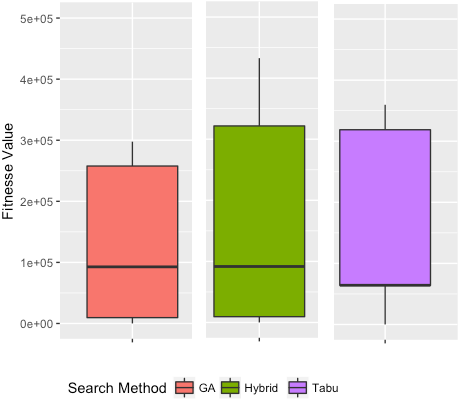
\includegraphics[width=0.8\textwidth]{./images/antipattern1.png}
\caption{Average, median, maximum and minimal fitness value by Search Method}
\label{fig:boxplot1}
\end{figure}

Table \ref{tab:bestindividuals} shows 4 best individuals found in the experiment by hybrid algorithm. None of the best individuals has one of the antipatterns used in the experiment, excluding the scenarios with antipatterns.

% Please add the following required packages to your document preamble:
% \usepackage[table,xcdraw]{xcolor}
% If you use beamer only pass "xcolor=table" option, i.e. \documentclass[xcolor=table]{beamer}
\begin{table}[h]
\centering
\caption{Best individuals found in the first experiment}
\label{tab:bestindividuals}
\begin{tabular}{lllll}
\rowcolor[HTML]{C0C0C0}
\textbf{Metaheur.} & \textbf{Gen.} & \textbf{Users} & \textbf{Fit} & \textbf{Scenarios}  \\
Hybrid & 17 & 145 & 432760 & Happy 1 \& 2  \\
Hybrid & 17 & 145 & 432740 & Happy 1 \& 2   \\
Hybrid & 17 & 146 & 431760 & Happy 1 \& 2  \\
Hybrid & 16 & 143 & 426740 & Happy 1 \& 2
\end{tabular}
\end{table}



\subsection{The Tower Babel  and Unbalanced Processing step}


The experiment was carried out for 6 continuous hours. In this experiment, Scenarios were generated with Tower Babel and Unbalanced Processing anti-pattern as well as scenarios with Happy Scenario 1, Happy Scenario 2 and mixed scenarios.

\begin{figure}[h]
\centering
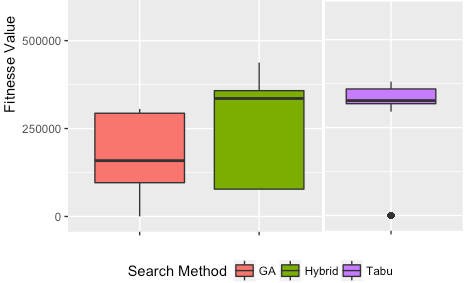
\includegraphics[width=0.8\textwidth]{./images/antipattern2.png}
\caption{Finesse value by generation in all tests}
\label{fig:boxplot2}
\end{figure}



Table \ref{tab:bestindividuals2} shows the 4 best workloads found in the second experiment. Despite the fact of doing 300 conversions of the JSON format to XML. The antipattern implementation does not return a higher response time than happy paths. While happy paths return from 10 to 15 seconds from a single user, Tower Babel antipattern has a response time of 10 to 29 seconds. None of the best individuals found implements the Unbalanced Processing antipattern.


% Please add the following required packages to your document preamble:
% \usepackage[table,xcdraw]{xcolor}
% If you use beamer only pass "xcolor=table" option, i.e. \documentclass[xcolor=table]{beamer}
\begin{table}[h]
\centering
\caption{Best individuals found by hybrid algorithm in the second experiment}
\label{tab:bestindividuals2}
\begin{tabular}{lllll}
\rowcolor[HTML]{FFCCC9}
\textbf{Metaheur.} & \textbf{Gen.} & \textbf{Users} & \textbf{Fit} & \textbf{Scenarios}  \\
\multicolumn{1}{l}{Hybrid} & \multicolumn{1}{l}{17} & \multicolumn{1}{l}{148} & \multicolumn{1}{l}{437780} & \multicolumn{1}{l}{Happy 1,2 \& Tower}  \\
\multicolumn{1}{l}{Hybrid} & \multicolumn{1}{l}{17} & \multicolumn{1}{l}{145} & \multicolumn{1}{l}{432740} & \multicolumn{1}{l}{Happy 1,2 \& Tower}  \\
\multicolumn{1}{l}{Hybrid} & \multicolumn{1}{l}{16} & \multicolumn{1}{l}{146} & \multicolumn{1}{l}{431800} & \multicolumn{1}{l}{Happy 1,2 \& Tower} \\
\multicolumn{1}{l}{Hybrid} & \multicolumn{1}{l}{17} & \multicolumn{1}{l}{145} & \multicolumn{1}{l}{428780} & \multicolumn{1}{l}{Happy 1,2 \& Tower}  \\
\end{tabular}
\end{table}

In the second experiment, the metaheuristics converged to scenarios with a happy path and Tower Babel anti-pattern, excluding the scenarios with Unbalanced Processing anti-pattern. The hybrid metaheuristic returned individuals with higher fitness scores. The SA algorithm obtained the worst fitness values.

\subsection{Threats to validity}
\begin{itemize}
\item Construct Validity:
In this experiment, we just evaluate the use of four antipatterns. However, several anti-patterns could be applied.  The common representation and the strategies used for crossover and neighborhood operators need a better design, using an abstraction pattern to contemplate a major number of possible solutions.
\item Conclusion Validity:
The Tower Babel anti-pattern was not excluded by the metaheuristics used in the experiment, requiring new studies with new approaches and experiments.
\end{itemize}


\section{Conclusion}

This chapter presented a hybrid metaheuristic approach for use in stress testing. Three experiments were performed to validate the solution. The first experiment was performed on an emulated component. The second experiment was performed using an installed Moodle application.  The collaborative approach obtained better fit values in both first two experiments.

The main contributions presented in this chapter are as follows: The presentation of a hybrid metaheuristic approach for use in stress tests; the development of a JMeter plugin  for search-based tests; and  the automation of the stress test execution process.

In the first experiment, the signed-rank Wilcoxon non-parametrical procedure was used for comparing the results. The significant level adopted was 0.05. The procedure showed that there was a significant improvement in the results with the Hybrid Metaheuristic approach.

In the second experiment, the whole process of stress and performance tests, which took 3 days and about 1800 executions, was carried out without the need for monitoring by a test designer. The tool automatically selected the next scenarios to be run up to the limit of six generations previously established.

The third experiment was conducted to validate the use of anti-patterns with the Hybrid algorithm. The experiments use genetic, algorithms, tabu search, simulated annealing and the hybrid algorithm.  We conducted the experiment in two steps in order to verify the effectiveness of the hybrid algorithm.  In the first step, none of the best workloads has one of the anti-pattern scenarios. In the second step,  the metaheuristics converged to scenarios with a happy path and Tower Babel antipattern, excluding the scenarios with Unbalanced Processing anti-pattern. In both experiments, the hybrid metaheuristic returned individuals with higher fitness scores. 


\chapter{Stress Search-based Testing using HybridQ approach}


This chapter presents a reinforcement learning approach to optimize the choice of neighboring solutions to explore, reducing the time needed to obtain the scenarios with the longest response time in the application.The research assumes that HybridQ is more expensive than Hybrid because q-learning. The research has as premise that the same application under performance tests can be submitted to more than one cycle of tests execution, reducing the cost of the exploration phase of the q-learning algorithm used. 


The solution, named HybridQ, uses the GA, SA and Tabu Search algorithms in a collaborative approach. Just like most reinforcement learning problems the proposed solution works in two different phases: exploration and exploitation. The following subsections show details of the exploration and exploitation phases and the integration between metaheuristics and the Q-Learning algorithm.


\subsection{Exploration phase}

The exploration phase uses a markov model, as shown in Fig. \ref{fig:mdphybridq}, the proposed MDP model  has three main states based on response time. A test may have a response time greater than 1.2 times the maximum response time allowed, between 0.8 and 1.2 times the maximum response time allowed or less than 0.8 times the maximum response time allowed. The values of 1.2 and 0.8 were chosen from the assumption of a tolerance margin of 20\% for the application under test. This margin may be higher or lower depending on the business requirements of the application.


\begin{figure}[h!]
\center
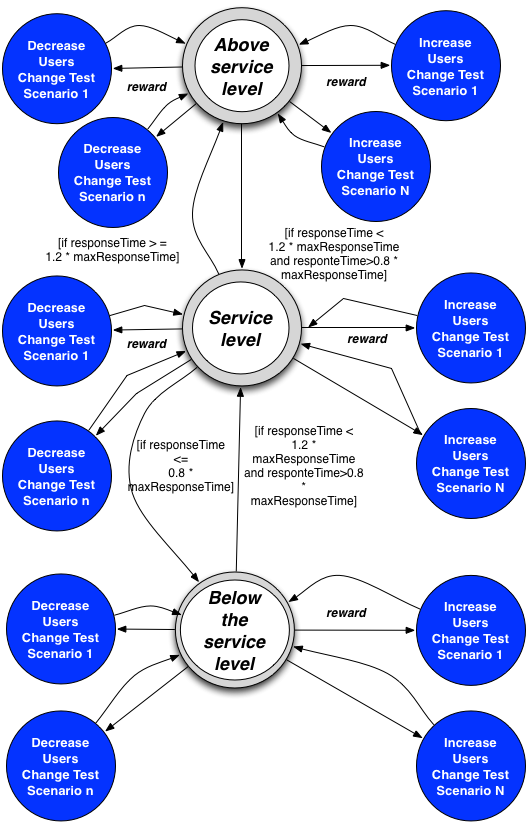
\includegraphics[width=0.4\textwidth]{./images/mdp3.png}
\caption{Markov Decision Process used by HybridQ}
\label{fig:mdphybridq}
\end{figure}


The algorithm maintains three different tables ( Table \ref{pab:mdp}), one for each state. The selection of which table to use depends on the response time of the application.

\begin{algorithm}[h]
  \caption{Exploration phase table selection }\label{hybridqexploration}
  \begin{algorithmic}[1]    
    \If {responseTime < 0.8 * maxResponseTime }
    \State return qTableBellowServiceLevel       
    \EndIf
     \If {responseTime >= 0.8 * maxResponseTime and responseTime <= 1.2* maxResponseTime}
    \State return qTableServiceLevel  
    \EndIf
    \If {responseTime > 1.2 * maxResponseTime}
    \State return qTableAboveServiceLevel  
    \EndIf
  \end{algorithmic}
\end{algorithm}

Algorithm \ref{hybridqexploration} shows the main steps of exploration phase. The possible actions in MDP are the change of one of the test scenarios and an increase or decrease in the number of users. In line 1, the algorithm choose a random action (increase, decrease or maintain the number of users). In line 2, the algorithm choose one a random testScenario. In lines 3 to 7, the algorithm checks if there exists a q value  for the pair (action and test scenario), if not exist a q value then zero value is assigned. In line 8, the algorithm checks i the new solution increases the fitness value. A solution receives a positive reward when an action increases the fitness value and a negative reward when an action reduces the fitness value.  Finally, the algorithm updates the qTable with the new q value.


\begin{algorithm}[h]
  \caption{HybridQ exploration phase }\label{hybridqexploration}
  \begin{algorithmic}[1]    
    \State $action \gets Random.createAction()$
    \State $testScenario \gets Random.chooseTestScenario()$
    \If {qTable.containsKey(action + "\#" + testScenario)}
    \State $ qValue \gets qTable.get(action + "\#" + testScenario);$
    \Else
        \State $ qValue \gets 0$
    \EndIf
     \If {newSolution.getFitness() > oldSolution.getFitness()}
     \State $qValue \gets ReinforcementLearning.alpha * reward + (1 - ReinforcementLearning.alpha) * qValue$     
     \Else
          \State $qValue \gets ReinforcementLearning.alpha * -reward + (1 - ReinforcementLearning.alpha) * qValue$     
    \EndIf     
    \State qTable.update(action + "\#" + testScenario, qValue)    
  \end{algorithmic}
\end{algorithm}

 

Unlike the traditional approach, The update of Q values for each action also occurs in the exploitation phase. The exploration phase ends when no value of Q equals zero for a state, ie, unlike the traditional approach an agent belonging to one state may be in the exploration phase while another agent may be in the exploitation phase. Table \ref{pab:mdp} presents hypothetical Q-values for a test. In Table \ref{pab:mdp}, it can be observed that the agents in the Service Level state are in the exploitation phase because there is no other value of Q that equals to zero.


% Please add the following required packages to your document preamble:
% \usepackage[table,xcdraw]{xcolor}
% If you use beamer only pass "xcolor=table" option, i.e. \documentclass[xcolor=table]{beamer}
\begin{table}[h]
\centering
\caption{Hypothetical MDP Q-values }
\label{pab:mdp}
\begin{tabular}{lll}
\rowcolor[HTML]{C0C0C0} 
\textbf{Above Service Level}  & \textbf{Scenario 1} & \textbf{Scenario 2} \\
Increment Users               & 0.2                 & 0.0                 \\
Reduce Users                  & 0.1                 & 0.2                 \\
Phase                         & Exploration         & Exploration         \\
\rowcolor[HTML]{C0C0C0} 
\textbf{Service Level}        & \textbf{Scenario 1} & \textbf{Scenario 2} \\
Increment Users               & 0.2                 & 0.11                \\
Reduce Users                  & 0.1                 & -0.2                \\
\rowcolor[HTML]{F8FF00} 
Phase                         & Exploitation         & Exploitation         \\
\rowcolor[HTML]{C0C0C0} 
\textbf{Bellow Service Level} & \textbf{Scenario 1} & \textbf{Scenario 2} \\
Increment Users               & 0.0                 & 0.2                 \\
Reduce Users                  & 0.1                 & 0.0                 \\
Phase                         & Exploration         & Exploration        
\end{tabular}
\end{table}

\subsection{Exploitation phase}

The main objective of the exploitation phase is to choose the best neighboring solution based on the Q value. The research expected that Q-Learning improve Hybrid algorithm replacing the random characteristic of the tabu search, simulated  annealing and genetic algorithms operators by the direction given by the q-learning in the exploration phase. Algorithm \ref{hybridqexploitation} presents the main steps of exploitation phase. In first line, the algorithm gets the original genome. In lines 2 to 11, HybridQ gets the maximum, the second maximum or the third maximum \textit{q} value, depending on the random value of the random variable.The algorithm chooses one of the three largest values of q. The variation of the highest values was inserted in the algorithm to escape the local optimals. In line 12, the algorithm gets the key value in Table that have the maximum \textit{q} value. In line number 13, The key is separated into two parts using the \# delimiter. The first part of the key is action and the second part is the test scenario. If the action equals '\textit{up}' value, the genome is incremented in its users. If the action equals '\textit{down}' value, the genome is incremented in its users. Finally, the test scenario is changed and the new genome is returned.




\begin{algorithm}[h]
  \caption{HybridQ exploitation phase }\label{hybridqexploitation}
  \begin{algorithmic}[1]    
    \State $Gene[] genome \gets service.getTestGenome()$
    \State $random \gets Random.nextInt(3)$
    \If {random==1}     
    \State $qMaxValue \gets qTable.getMaxValue(responseTime)$
    \EndIf
    \If {random==2}     
    \State $qMaxValue \gets qTable.getSecondMaxValue(responseTime)$
    \EndIf
    \If {random==3}     
    \State $qMaxValue \gets qTable.getThirdMaxValue(responseTime)$
    \EndIf
    \State $key \gets qTable.selectKey(qMaxValue)$
    \State $String[]\  keySplit \gets key.split('\#')$ 
    \State $action \gets keySplit[0]$
    \State $testScenario \gets keySplit[1]$   
    \If {action=='up'}
    \State $ increaseUsers(genome) $
    \EndIf
    \If {action=='down'}
    \State $ decreaseUsers(genome) $
    \EndIf    
    \State $genomePosition \gets Random.nextInt(genome.length)$
    \State changeTestScenario(genome,testScenario,genomePosition)
  \end{algorithmic}
\end{algorithm}

\subsection{Integration between metaheuristics and the Q-Learning algorithm }

The Q-learning algorithm is used by Tabu Search or Simulated Annealing to obtain the neighbors and in the mutation operator of the genetic algorithm. Unlike the traditional processes of obtaining neighboring solutions such as random change and permutation, the decision to change a genome gene is made from the action that has the highest value of Q. Fig. \ref{fig:neighservice} presents how one of the neighbors of a test is generated using Q-Learning in IAdapter. The solution uses a service called Q-Neighborhood Service to generate the neighbor from the action that has the highest value of Q.

\begin{figure}[h!]
\center
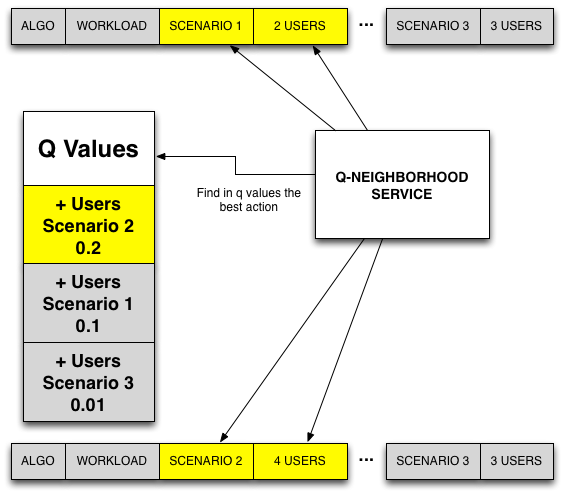
\includegraphics[width=0.6\textwidth]{./images/q-neighborservice.png}
\caption{HybridQ Neighborhood Service}
\label{fig:neighservice}
\end{figure}

\section{Experiment with HybridQ Algorithm}

We conducted one experiment in order to verify the effectiveness of the HybridQ. The iterated racing procedure (irace) was applied as an automatic algorithm configuration tool for tunning metaheuristics parameters. Iterated racing is a generalization of the iterated F-race procedure to automatize the arduous task of configuring the parameters of an optimization algorithm \cite{ManuelLopez-IbanezJeremieDubois-LacosteLesliePerezCaceresMauroBirattari2016}. The best parameters obtained from irace was a population size of 5 individuals, a crossover value of 0.7551, a mutation value of 0.7947, an elitism value of 0.5356 and the maximum number of iterations of 16. The experiment ran for 16 generations in an docker environment on a server with 16 Gb of memory and 500 Gb hard disk. The experiment used an initial population of 5 individuals by metaheuristics. The genetic algorithm used the top 4 individuals from each generation in the crossover operation. The Tabu list was configured with the size of 10 individuals and expired every 2 generations.  The mutation operation was applied to 79\% of the population on each generation. The experiments use tabu search, genetic algorithms, simulated annealing, the hybrid metaheuristic approach and the HybridQ approach. 


The objective function applied is intended to maximize the response time of the scenarios being tested.  In these experiments, better fitness values coincide with finding scenarios with higher values of response time. A penalty is applied when the response time is greater than the  maximum response time expected. The experiment used the following fitness (goal) function:

\begin{equation}
\begin{aligned}
fitness=
20* 90percentiletime\\
20*80percentiletime\\
20*70percentiletime\\
20*maxResponseTime\\
-penalty
\end{aligned}
\end{equation}

For the experiment an objective function with a single factor was chosen, since users and response time are conflicting factors. All tests in the experiment were conducted without the need of a tester, automating the process of executing and designing performance test scenarios.    

\subsection{Experiment Research Questions}

The following research question is addressed:

\begin{itemize}
\item Is Q-learning technique improve the choice of neighboring solutions, improving the number of requests and the time needed to find scenarios with the longest response time in the application under test?
\end{itemize}

\subsection{Variables}

The independent variable is the algorithms used in each experiment. The dependent variables are: the optimal solution found by each algorithm, the number of requests to find optimal solution and the time of execution needed by each algorithm.

\subsection{Experiment Hypotheses}

\begin{itemize}
\item With regard to the optimal solution found by each algorithm:
\begin{itemize}
\item $H1_{0}$ (null hypothesis) : The HybridQ does not find better solution than the other metaheuristic approaches.
\item $H1_{1}$  : The HybridQ finds better solution than the one discovered by other metaheuristic approaches.
\end{itemize}
\end{itemize}


\begin{itemize}
\item With regard to the time consumed to find the optimal solution of each algorithm:
\begin{itemize}
\item $H2_{0}$ (null hypothesis) : The HybridQ algorithm realizes more requests than the other algorithms in the experiments performed.
\item $H2_{1}$  : The HybridQ algorithm does not realize more requests than the other algorithms in the executed experiments.
\end{itemize}
\end{itemize}


\begin{itemize}
\item With regard to the number of requests needed to find the optimal solution of each algorithm:
\begin{itemize}
\item $H3_{0}$ (null hypothesis) : The HybridQ algorithm needs more time to find the optimal solution than the other algorithms in the experiments performed.
\item $H3_{1}$  : The HybridQ algorithm does not need more time to find the optimal solution than the other algorithms in the experiments performed.
\end{itemize}
\end{itemize}

\subsection{Experiment phases}

The experiment was conducted in two phases. The first phase verified the number of requisitions and time required for the HybridQ exploration phase. The second phase ran the stress test using GA, Tabu Search, Simulated Annealing, Hybrid and HybridQ algorithms simultaneously.

\subsection{OpenCart Experiment}

The experiment was conducted to test the use of the HybridQ algorithm in a real implemented application.  The chosen application was the OpenCart application , available at \url{opencart.com}. OpenCart is free open source ecommerce platform for online merchants. OpenCart works with PHP 5 and MySQL. The maximum tolerated response time in the test was 5 seconds. The whole process of stress and performance tests, which run for 2 days and  with about 1.500 executions, was carried out without the need for monitoring by a test designer. The tool automatically selected the next scenarios to be run up to the limit of eleven generations previously established. 

The experiments use the follow application features:

\begin{itemize}
\item Main page: The main page of the application.
\item Search item: The application searches a product.
\item Product detail: The application shows  details about one item product.
\item Add to Cart: The application adds a product to shopping cart.
\item View Cart:The application displays the shopping cart.
\item Remove Item: The application remove item from shopping cart. 
\end{itemize}

\subsubsection{Q-Learning Training Phase}

The application was submitted to 1 hour of training with the  Q-learning algorithm using all test scenarios  and was obtained the Table \ref{tab:opencartlearning1} with the values of \textit{q}  for response times bellow than service level. The action and state with best q-value is increment the number of users ('up') in Add to Cart feature. The learning phase required 1.431 requisitions for application under test. 


% Please add the following required packages to your document preamble:
% \usepackage[table,xcdraw]{xcolor}
% If you use beamer only pass "xcolor=table" option, i.e. \documentclass[xcolor=table]{beamer}
\begin{table}[]
\centering
\caption{Q values for response times bellow than service level}
\label{tab:opencartlearning1}
\begin{tabular}{|l|l|l|l|l|l|}
\hline
\rowcolor[HTML]{EFEFEF} 
\textbf{Action} & \textbf{Feature} & \textbf{Q- value} & \textbf{State}                      & \textbf{Feature}                             & \textbf{Q- value}                          \\ \hline
up              & Main Page        & -0.0405763        & \cellcolor[HTML]{EFEFEF}\textbf{up} & \cellcolor[HTML]{EFEFEF}\textbf{Add to Cart} & \cellcolor[HTML]{EFEFEF}\textbf{0.0390237} \\ \hline
down            & Main Page        & 0.00079202        & down                                & Add to Cart                                  & -0.00079202                                \\ \hline
same            & Main Page        & -0.0398           & same                                & Add to Cart                                  & -0.0398                                    \\ \hline
up              & Search Page      & -0.00079202       & up                                  & View Cart                                    & -0.0398                                    \\ \hline
down            & Search Page      & -0.0398           & down                                & View Cart                                    & -0.0398                                    \\ \hline
same            & Search Page      & -0.0398           & same                                & View Cart                                    & -0.0398                                    \\ \hline
up              & Product Detail   & -0.00079202       & up                                  & Remove Item                                  & -0.0398                                    \\ \hline
down            & Product Detail   & -0.00079202       & down                                & Remove Item                                  & -0.0398                                    \\ \hline
same            & Product Detail   & -0.0398           & same                                & Remove Item                                  & -0.0398                                    \\ \hline
\end{tabular}
\end{table}

\subsubsection{Results}

Figure \ref{fig:experiment1} presents the number of requests by maximum fitness value. HybridQ algorithm obtains the maximum value of fitness: 364860 ($H1_{1}$ hypothesis).  HybridQ obtained a solution with greater fitness value, but it needs a much greater number of requests than the other algorithms, not contemplating the hypothesis $H2_{1}$. GA is the algorithm that obtain the best fitness value with minor number of requests ($H1_{0}$ hypothesis). All algorithms consume the same time of test (6 hours). The scenario with more fitness value has 4,8 seconds of response time and 38 users:

\begin{itemize}
\item 25 users on search page;
\item 10 users on Add to Cart feature;
\item 2 users removing items from cart;
\item 1 users on Main Page. 
\end{itemize}

\begin{figure}[h]
\centering
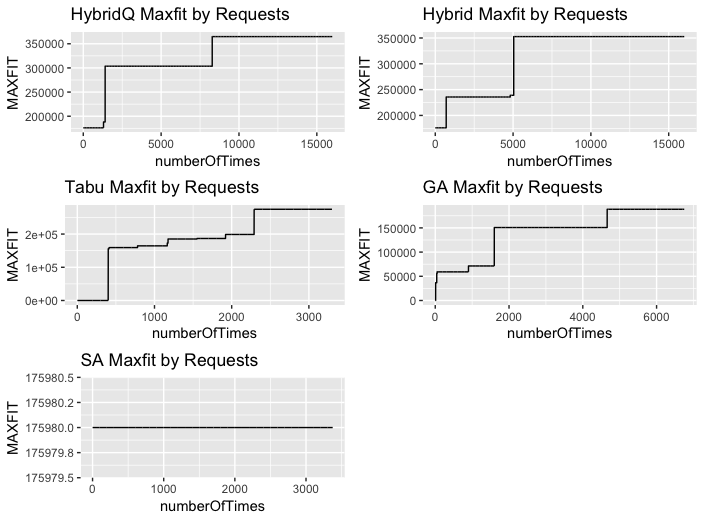
\includegraphics[width=1\textwidth]{./images/experiment1.png}
\caption{Maximum fitness value by number of requests}
\label{fig:experiment1}
\end{figure}


The t-Test and Wilcoxon Rank Sum Test was applied using the R language. The test results show that HybridQ and HybridQ algorithms is superior than GA, Tabu Search and Simulated Annealing with p < 0.02. t-Test shows that the mean of HybridQ fitness value is superior than Hybrid.

\begin{lstlisting}
	Welch Two Sample t-test

data:  b\$MAXFIT and c\$MAXFIT
t = 13.829, df = 31678, p-value < 2.2e-16
alternative hypothesis: true difference in means is not equal to 0
95 percent confidence interval:
 7506.846 9986.226
sample estimates:
mean of x mean of y 
 332007.5  313260.9 

\end{lstlisting}



\subsection{Threats to validity}

In this work, we just evaluate the use of single objective algorithm. However, several multiobjective algorithms could be applied.  The experiments are performed with the configuration obtained by the irace algorithm, however new experiments are required to verify the sensitivity of the results. It is necessary to compare the current approach with the constraint programming approaches presented in the state of art.



\section{Conclusion}

The present study extends the article "Improving stress search based testing using a hybrid metaheuristic approach" in order to ascertain if the use of the Q-learning technique allows the meta-heuristic algorithms to improve the search for application failures One experiment was conducted to validate the proposed approach. The experiments use genetic algorithms, tabu search, simulated annealing, the hybrid approach and the HybridQ algorithm. The experiment ran for 17 generations. The experiment used an initial population of 5 individuals by metaheuristics. All tests in the experiment were conducted without the need of a tester, automating the execution of stress tests with the JMeter tool.  HybridQ found the individuals with a greater response time. The scenario with greater fitness has 38 users with the Search Page, Add to Cart feature, Removing Item and Main Page features. GA is the algorithm that obtain the best fitness value with minor number of requests. All algorithms consume the same time of test (6 hours). 


\FloatBarrier

\chapter{Search-based stress testing using multi-objective heuristics}

This chapter present experiments to assert the benefits of multiobjective metaheuristics in search-based stress testing. Multi-objective heuristics may be more suitable for non-functional search-based tests since these tests usually aim to obtain a result with more than one objective, for example, minimizing the number of users of an application, maximize your response time. We examine the use of the multi-objective NSGA-II, SPEA2, PAES and MOEA/D algorithms. The multi-objective algorithms applied in the experiments use an adapted implementation of the jMetal framework (\url{http://jmetal.sourceforge.net/}). Figure. \ref{fig:flowchart} presents the flowchart of  Multiobjective Algorithms Adaptation. Given an initial population (Figure \ref{fig:flowchart}  -\ding{202}),  the multiobjective algorithm implementation receives a set of workloads  and generates a new set of individuals  (Figure \ref{fig:flowchart}  -\ding{203}).  JMeterEngine runs each workload (Figure \ref{fig:flowchart}  -\ding{204}) and the multiobjective algorithm ranks and classifies each workload based on the objective functions  (Figure \ref{fig:flowchart}  -\ding{205}).  After all these steps the cycle begins until the maximum number of generations is reached.

\begin{figure}[!h]
\centering
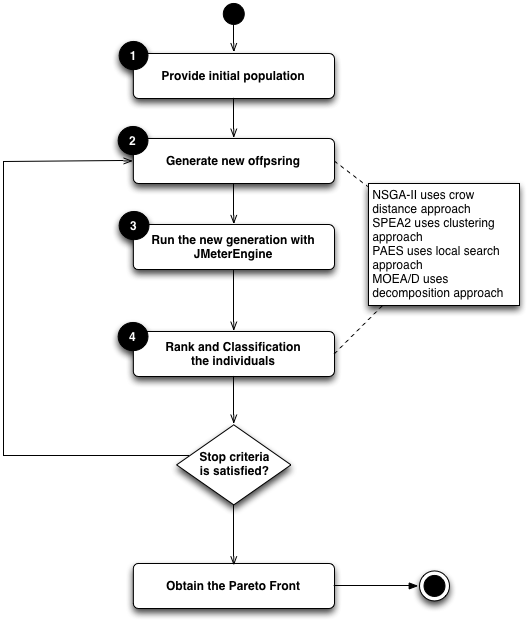
\includegraphics[width=0.8\textwidth]{./images/step3.png}
\caption{Flowchart of implemented algorithms}
\label{fig:flowchart}
\end{figure}


Several experiments were performed to evaluate the use of multi-objective metaheuristics in search-based stress testing. The experiments use the SEDR adaptation presented in Appendix B. The first experiment uses NSGA-II algorithm to discover application scenarios where there is a high response time for a small number of users. The second experiment presents the experimental results to compare the four multi-objective algorithms.  MOEA/D metaheuristics obtained the best hypervolume value when compared with other approaches. Consequently, we propose a collaborative approach using MOEA/D and HybridQ to improve the hypervolume values obtained from the previous experiments. Each algorithm shares our best individuals with each other. The fourth experiment presents an experiment to assess the collaborative approach using HybridQ and MOEA/D. 

Due to the pervasive and non-deterministic nature of the problem, we do not guarantee that the same Pareto frontier will be found in different test executions. The fifth experiment presents an initial study to evaluate the Pareto Frontier difference in multiple executions. 

\section{Experiment with multi-object NSGA-II algorithm}

In this section,  we present the experimental results,  in which we carried out to verify the multi-objective NSGA-II   implementation. This experiment runs to verify the feasibility of using multi-objective heuristics in search-based stress testing. NSGA-II was initially used for its ease of implementation. This experiment tries to discover application scenarios where there is a high response time for a small number of users. The relevance of finding scenarios with superior response times is to enable corrective actions before the application under test is released in a production environment. The chosen application was the JPetStore, available at \url{https://hub.docker.com/r/pocking/jpetstore/}. The maximum tolerated response time in the test was 500 milliseconds.  The whole process of stress  tests, which run for 3 days and 492 executions,  was conducted without the need for monitoring by a test designer. The tool automatically selected the next scenarios to be run up to the limit of 123 previously established  generations by the algorithm. The experiments use the following application features:


\begin{itemize}
\item Enter in the Catalog: the application presents the catalog of pets.
\item Fish: The application shows all the fish items in stock.
\item Register:  a new user is registered into the system.
\item Dogs: The application shows all the dog supplies in stock.
\item Shopping Cart: the application displays the shopping cart.
\item Add or Remove to Shopping Cart: the application adds and removes items from the shopping cart.
\end{itemize}

The experiments used an initial population of 17 individuals by metaheuristic. The genetic algorithm used the top 10 individuals from each generation in the crossover operation  The mutation operation was applied to 10\% of the population in each generation. The objective function applied is intended to minimize the number of users and maximize the response time of the scenarios being tested. A penalty applies if an application under test takes a longer time to respond than the expected maximum response time. The experiment used the following objective equations:

\begin{equation}
\begin{aligned}
objective function 1 =numberOfUsers\\
-penalty\\
\end{aligned}
\end{equation}


\begin{equation}
\begin{aligned}
objective function 2 =responsetime\\
-penalty\\
\end{aligned}
\end{equation}

The first objective function seeks to find workloads with fewer users. The second objective function seeks to find workloads with longer response times. The penalty is calculated by the following equation:

\begin{equation}
\begin{aligned}
penalty=100 * \Delta \\
\Delta=(t_{Current Response Time} - t_{Maximum Response Time Expected})\\
\end{aligned}
\end{equation}



\subsection{Experiment Research Questions}

The following research question is addressed:
\begin{itemize}
\item Does the NSGA-II algorithm find relevant workload scenarios according to the two test objectives?
\end{itemize}

\subsection{Variables}

The independent variable is the use (or not) of NSGA-II algorithm. The dependent variables are the optimal workload scenario found by the algorithm.

\subsection{Experiment Hypotheses}

\begin{itemize}
\item With regard to multi-objective algorithms applied in the experiment:
\begin{itemize}
\item $H_{0}$ (null hypothesis): The NSGA-II didn't find workloads that meet the two objective functions used in the experiment.
\item $H_{1}$: The NSGA-II  algorithm found workloads that meet the two objective functions used in the experiment.
\end{itemize}
\end{itemize}


\subsection{Results}

Fig. \ref{fig:paretofrontier1} and Table \ref{tab:results} present the results obtained in the experiment. The experiment found 9 optimal workloads (Pareto Frontier) that present a lower number of users with high response times. Workload number 1 with a single user accessing the dog scenario provided a response time of 245 milliseconds.  Workload number 2 with a single user accessing the dog scenario, 7 users accessing the Enter Catalog feature and 3 users in register functionality, provided a response time of 400 seconds.



\begin{figure}[h]
\centering
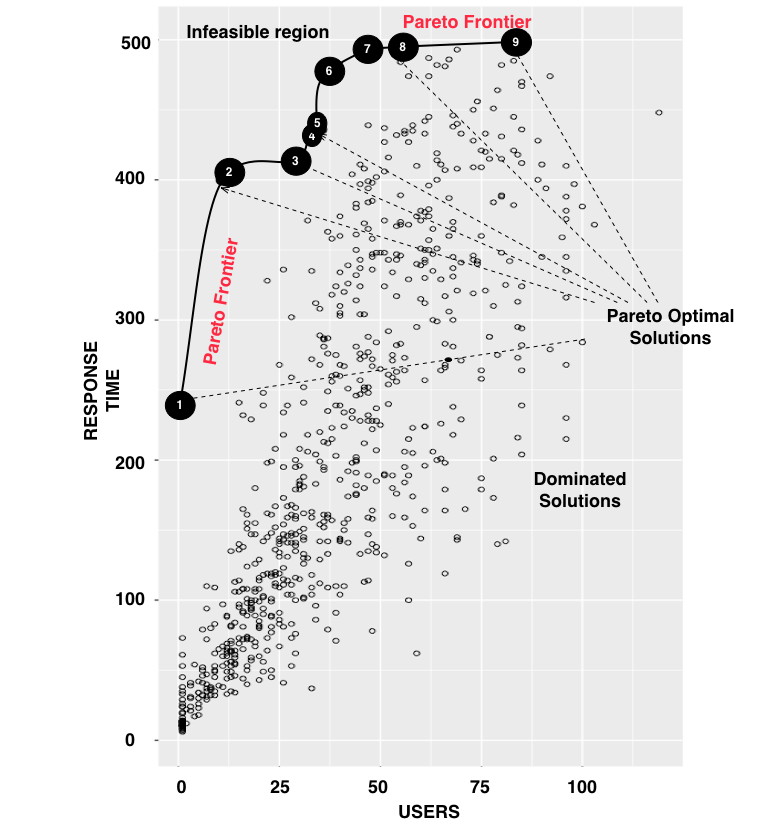
\includegraphics[width=0.8\textwidth]{./images/pareto0curve.png}
    \caption{Pareto Frontier found in the first experiment using NSGA-II}
\label{fig:paretofrontier1}
\end{figure}

% Please add the following required packages to your document preamble:
% \usepackage[table,xcdraw]{xcolor}
% If you use beamer only pass "xcolor=table" option, i.e. \documentclass[xcolor=table]{beamer}
\begin{table}[!h]
\centering
\caption{Response time and number of users in optimal scenarios found with NSGA-II}
\label{tab:results}
\begin{tabular}{|l|l|l|l|l|l|l|l|l|}
\hline
\rowcolor[HTML]{C0C0C0}
\textbf{N.} & \textbf{\begin{tabular}[c]{@{}l@{}}USERS\\ \end{tabular}} & \textbf{\begin{tabular}[c]{@{}l@{}}RESP \\ TIME\end{tabular}} & \multicolumn{1}{c|}{\cellcolor[HTML]{C0C0C0}\textbf{\begin{tabular}[c]{@{}c@{}}Dogs\\ Users\end{tabular}}} & \textbf{\begin{tabular}[c]{@{}l@{}}Enter\\ Catalog\\ Users\end{tabular}} & \textbf{\begin{tabular}[c]{@{}l@{}}Fish\\ Users\end{tabular}} & \textbf{\begin{tabular}[c]{@{}l@{}}Register\\ Users\end{tabular}} & \textbf{\begin{tabular}[c]{@{}l@{}}Add\\ Rem.\\ Cart\end{tabular}} & \textbf{\begin{tabular}[c]{@{}l@{}}Cart\\ Users\end{tabular}} \\ \hline
\ding{202}           & 1                                                        & 245                                                        & 1                                                          &                                                                  &               &                   &                                                                    &               \\ \hline
\ding{203}           & 11                                                       & 400                                                        & 1                                                          & 7                                                                &               & 3                 &                                                                    &               \\ \hline
\ding{204}           & 29                                                       & 416                                                        & 5                                                          & 15                                                               & 4             & 5                 &                                                                    &               \\ \hline
\ding{205}          & 34                                                      & 434                                                        & 16                                                         & 17                                                               &               &                   &                                                                    & 1             \\ \hline
\ding{206}           & 35                                                      & 436                                                        & 15                                                         & 4                                                                & 8             & 3                 & 5                                                                  &               \\ \hline
\ding{207}           & 37                                                      & 472                                                        & 7                                                          & 13                                                               & 7             & 3                 & 7                                                                  &               \\ \hline
\ding{208}           & 47                                                      & 493                                                        & 7                                                          & 11                                                               & 11            & 7                 & 7                                                                  & 4             \\ \hline
\ding{209}           & 54                                                      & 496                                                        & 6                                                          &                                                                  & 12            & 8                 & 19                                                                 & 9             \\ \hline
\ding{210}           & 85                                                      & 499                                                        &                                                            & 54                                                               & 12            &                   & 7                                                                  & 12            \\ \hline
\end{tabular}
\end{table}


\subsection{Threats to Validity}

In this work, we just evaluate the use of one multi-objective algorithm. However, several multi-objective algorithms could be applied.  There is still a reasonable distance between the Pareto frontier and the data obtained for the second objective, and more experiments are needed to validate the results.

\subsection{Experiment Conclusion}


The experiment verified the use of a multi-objective algorithm in a search-based stress testing problem. The experiment uses the NSGA-II algorithm to discover application scenarios where there is a high response time for a small number of users. The experiment found 9 optimal workloads that present a lower number of users with high response times. The results of the experiment can help in the decision making of service levels that need to be defined for the application.

\section{Comparative experiment of Multi-Objective Algorithms}


In this section, we present the experimental results, in which we carried out to compare four multi-objective algorithms:

\begin{itemize}
\item NSGA-II
\item SPEA2
\item PAES
\item MOEAD
\end{itemize}

The experiment was undertaken with the JPetStore application with and without a noise reduction strategy. The maximum tolerated response time in the test was 1000 milliseconds.  The whole process of stress tests, which run for 5 days and 2226 executions, was carried out without the need for monitoring by a test designer. The tool automatically selected the next scenarios to be run up to the limit of 50 previously established generations by the algorithm. The hypervolume metric was used to compare the algorithms.  All values used in the hypervolume calculation were normalized. We used the emoa package of the R language to calculate the hypervolume.

\subsection{Experiment Research Questions}

The following research question is addressed:
\begin{itemize}
\item Which, among the four algorithms chosen, is the most suitable multi objective algorithm for the search-based test problem?
\end{itemize}

\subsection{Variables}

The independent variable is the algorithms: NSGA-II, SPEA2, PAES and MOEA/D. The dependent variables are the hypervolume of each algorithm.

\subsection{Experiment Hypotheses}

\begin{itemize}
\item With regard to the relevance of test results:
\begin{itemize}
\item $H_{0}$ (null hypothesis): The multi-objective with the higher value of hypervolume don't find the scenarios with higher response time and lower number of users.
\item $H_{1}$: The multi-objective with  the higher value of hypervolume find the scenarios with higher response time and lower number of users.
\end{itemize}
\end{itemize}

\begin{itemize}
\item With regard to hypervolume of multi-objective algorithms applied in the experiment:
\begin{itemize}
\item $H_{1}$: MOEA/D is the algorithm with the higher value of hypervolume in the experiments.
\item $H_{2}$: NSGA-II is the algorithm with the higher value of hypervolume in the experiments.
\item $H_{3}$: SPEA2 is the algorithm with the higher value of hypervolume in the experiments.
\item $H_{4}$: PAES is the algorithm with the higher value of hypervolume in the experiments.
\end{itemize}
\end{itemize}


\subsection{Experiment Results}

Table \ref{tab:hypervolume} shows the hypervolume value of each algorithm. Dimensionality shows the number of dimensions used in the calculation of hypervolume. For the hypervolume calculus, the values of the number of users and response time were transformed to the same scale. The highest hypervolume algorithm was the MOEA/D. 
Table \ref{tab:results2} presents the test scenarios found in the Pareto frontier of MOEA/D.

% Please add the following required packages to your document preamble:
% \usepackage[table,xcdraw]{xcolor}
% If you use beamer only pass "xcolor=table" option, i.e. \documentclass[xcolor=table]{beamer}
\begin{table}[!h]
\centering
\caption{Response time and number of users in optimal scenarios found with MOEA/D}
\label{tab:results2}
\begin{tabular}{|l|l|l|l|l|l|l|l|l|}
\hline
\rowcolor[HTML]{C0C0C0}
\textbf{N.} & \textbf{\begin{tabular}[c]{@{}l@{}}USERS\\ \end{tabular}} & \textbf{\begin{tabular}[c]{@{}l@{}}RESP \\ TIME\end{tabular}} & \multicolumn{1}{c|}{\cellcolor[HTML]{C0C0C0}\textbf{\begin{tabular}[c]{@{}c@{}}Dogs\\ Users\end{tabular}}} & \textbf{\begin{tabular}[c]{@{}l@{}}Enter\\ Catalog\\ Users\end{tabular}} & \textbf{\begin{tabular}[c]{@{}l@{}}Fish\\ Users\end{tabular}} & \textbf{\begin{tabular}[c]{@{}l@{}}Register\\ Users\end{tabular}} & \textbf{\begin{tabular}[c]{@{}l@{}}Add\\ Rem.\\ Cart\end{tabular}} & \textbf{\begin{tabular}[c]{@{}l@{}}Cart\\ Users\end{tabular}} \\ \hline
\ding{202}           & 1                                                        & 18                                                       &                                                           & 1                                                                 &               &                   &                                                                    &               \\ \hline
\ding{203}           & 5                                                       & 35                                                        & 1                                                          &                                                                &               & 3                 &                                                                    & 1              \\ \hline
\ding{204}           & 6                                                       & 50                                                        & 2                                                          &                                                                &               & 3                 &                                                                    & 1              \\ \hline
\ding{205}           & 7                                                       & 320                                                        &                                                           &                                                                &               & 3                 &                                                                    & 4              \\ \hline
\ding{206}           & 12                                                       & 410                                                        &                                                           &                                                                &               & 3                 &  5                                                                  & 4              \\ \hline
\ding{207}           & 22                                                       & 788                                                        &                                                           &                                                                & 7             &     7             &    3                                                                & 5              \\ \hline
\ding{208}          & 72                                                      & 1074                                                        & 17                                                        & 19                                                                & 14              &  11             &                                                                    & 11            \\ \hline
\ding{209}           & 89                                                      & 1396                                                        & 8                                                         & 7                                                               & 10             &                 & 29                                                                  & 35              \\ \hline
\end{tabular}
\end{table}


MOEA/D found two scenarios that approached the established service level for the experiment of 1000 milliseconds. NSGA-II  found a scenario with 49 users and response time of 685 and a scenario with 59 users and response time of 1138 milliseconds. Although the MOEA/D algorithm found the scenario with the lowest number of users with a time close to the service level, the NSGA-II found a scenario with more users with a response time closer to the service level. Figures \ref{fig:moeadnoise}, \ref{fig:paretofrontier2}, \ref{fig:spea2} and  \ref{fig:paes} present the Pareto frontier for each algorithm. Fig. \ref{fig:comparative3} presents a comparative graph between all the algorithms.

% Please add the following required packages to your document preamble:
% \usepackage[table,xcdraw]{xcolor}
% If you use beamer only pass "xcolor=table" option, i.e. \documentclass[xcolor=table]{beamer}
\begin{table}[]
\centering
\caption{Hypervolume by algorithm}
\label{tab:hypervolume}
\begin{tabular}{|l|l|l|l|}
\hline
\rowcolor[HTML]{EFEFEF} 
\textbf{ALGORITHM} & \textbf{HYPERVOLUME} & \textbf{DIMENSIONALITY} & \textbf{POINT DENSITY} \\ \hline
MOEA/D             & 10.185576            & 2                       & 7817.328935            \\ \hline
NSGA-II            & 7.541011             & 2                       & 7726.815663            \\ \hline
PAES               & 7.240581             & 2                       & 7758.493105            \\ \hline
SPEA2              & 5.539566             & 2                       & 7772.269274            \\ \hline
\end{tabular}
\end{table} 

\begin{figure}[h]
\begin{minipage}{.5\textwidth}
\centering
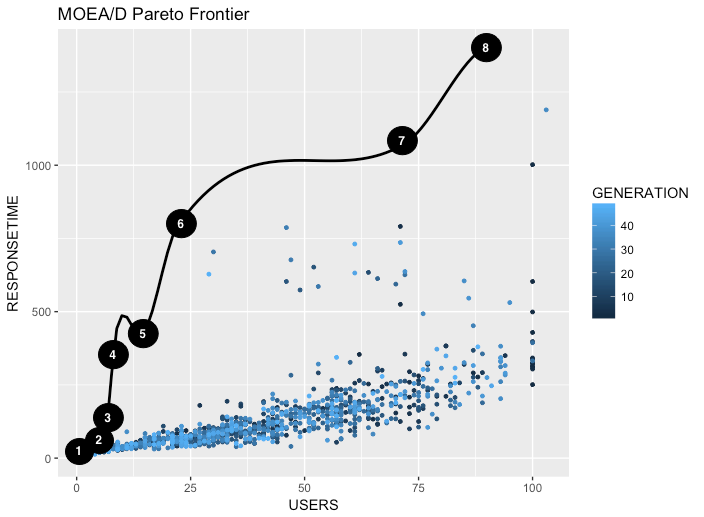
\includegraphics[width=1\textwidth]{./images/moeadnoise.png}
\caption{MOEA/D Pareto Frontier}
\label{fig:moeadnoise}
\end{minipage}
\begin{minipage}{.5\textwidth}
\centering
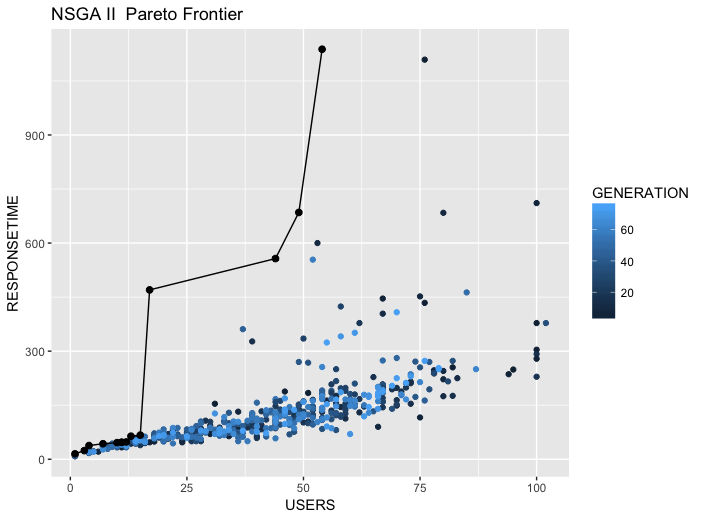
\includegraphics[width=1\textwidth]{./images/nsgaiinoise.png}
\caption{NSGA II Pareto Frontier}
\label{fig:paretofrontier2}
\end{minipage}
\end{figure}


\begin{figure}[h]
\begin{minipage}{.5\textwidth}
\centering
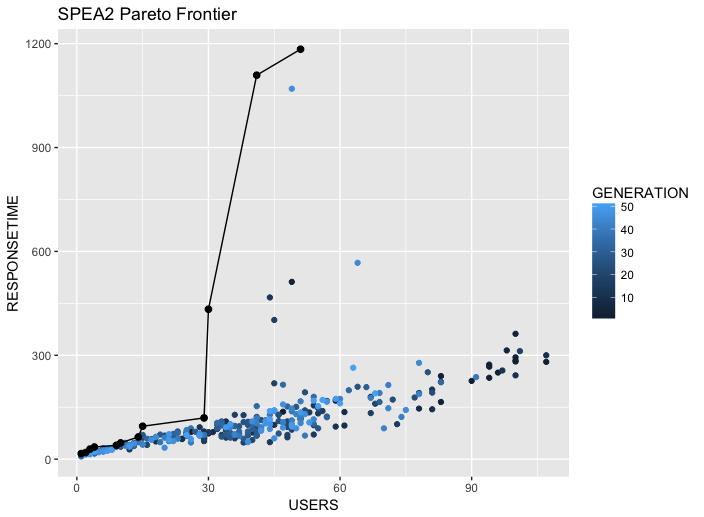
\includegraphics[width=1\textwidth]{./images/spea2noise.png}
\caption{SPEA2 Pareto Frontier}
\label{fig:spea2}
\end{minipage}
\begin{minipage}{.5\textwidth}
\centering
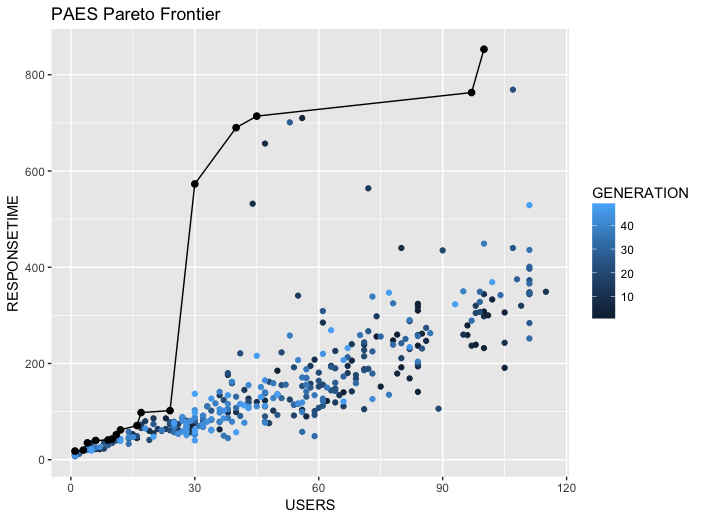
\includegraphics[width=1\textwidth]{./images/paesnoise.png}
\caption{PAES Pareto Frontier}
\label{fig:paes}
\end{minipage}
\end{figure}

\begin{figure}[h]
\centering
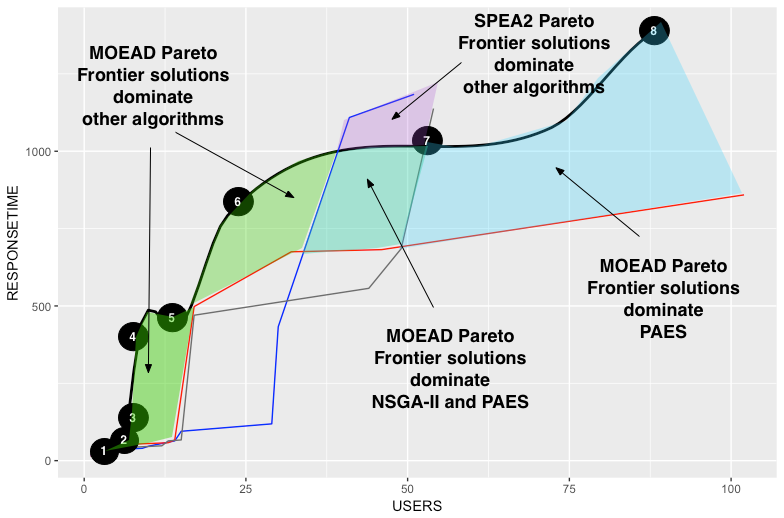
\includegraphics[width=1\textwidth]{./images/comparative3.png}
\caption{Comparative graph between MOEA/D, NSGA-II, SPEA2 and PAES Pareto Frontiers}
\label{fig:comparative3}
\end{figure}

\subsection{Experiment Conclusion}

The multi-objective with the higher value of hypervolume find the scenarios with higher response time and lower number of users. However, each algorithm presented relevant results for stress testing. MOEA/D was the algorithm with the highest hypervolume value.

\subsection{Threats to Validity}

Due to the non-deterministic nature of the problem, we do not guarantee that the same Pareto frontier will be found in different test executions. The workloads found by the MOEA/D algorithm  do not dominate all workloads found by all others algorithms.


\section{Comparative Experiment between HybridQ and MOEA/D}

This section presents the experimental results carried out to compare the MOEA/D multi-objective with the HybridQ algorithm. The experiment was conducted with the JPetStore application with the SEDR adapted  noise reduction strategy. The maximum tolerated response time in the test was 1000 milliseconds.  The whole process of stress  tests, which run for 1 day and 534 executions, was carried out without the need for monitoring by a test designer. The tool automatically selected the next scenarios to be run up to the limit of 15 previously established  generations by the algorithm. 

\subsection{Experiment Research Questions}

The following research question is addressed:
\begin{itemize}
\item The solutions presented by a single objective algorithm are dominated by all solutions presented by a multi-objective algorithm?
\end{itemize}

\subsection{Variables}

The independent variable is algorithms: HybridQ and MOEA/D. The dependent variables are the Pareto frontier points found by each algorithm.

\subsection{Experiment Hypotheses}

\begin{itemize}
\item With regard to multi-objective and single objective algorithms applied in the experiment:
\begin{itemize}
\item $H_{0}$ (null hypothesis): All solutions found by HybridQ are not dominated by the MOEA/D algorithm.
\item $H_{1}$: All solutions found by HybridQ are dominated by the MOEA/D algorithm.
\end{itemize}
\end{itemize}

\subsection{Experiment Results}

Fig. \ref{fig:singlewithmulti} presents the result of the experiment. Most of the individuals found by the HybridQ algorithm are dominated by those found by MOEA/D. The exception is a single maximum point found by HybridQ. From the results, a hybrid collaborative approach was proposed, where the results between the MOEA / D and HybridQ algorithms would be shared. 


\begin{figure}[h]
\centering
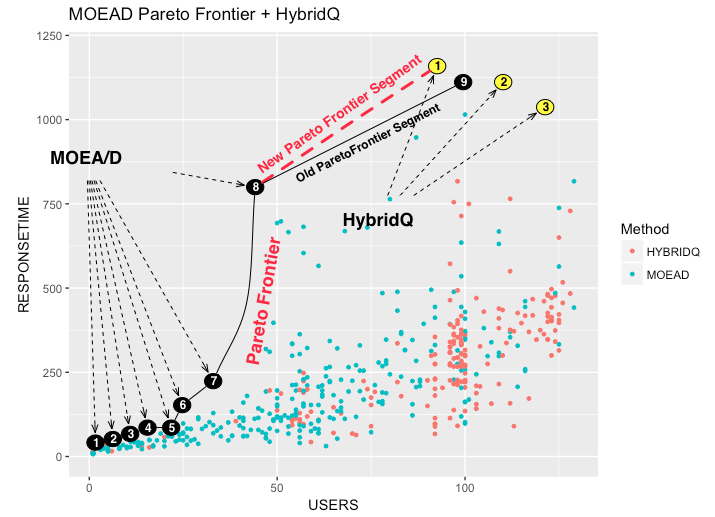
\includegraphics[width=1\textwidth]{./images/singlewithmulti.png}
    \caption{HybridQ and MOEA/D Pareto Frontier}
\label{fig:singlewithmulti}
\end{figure}

\section{Experiment with HybridQ and MOEA/D Collaborative approach}

This section presents an experiment to evaluate the collaborative approach using HybridQ and MOEA/D. The proposition consists of each algorithm share our best individuals with each other. The experiment was conducted with the JPetStore application with the SEDR adapted  noise reduction strategy. The maximum tolerated response time in the test was 1000 milliseconds.  The whole process of stress  tests, which run for 1 day and 983 executions, was carried out without the need for monitoring by a test designer. The tool automatically selected the next scenarios to be run up to the limit of 50 previously established  generations by the algorithm.

\begin{figure}[h]
\centering
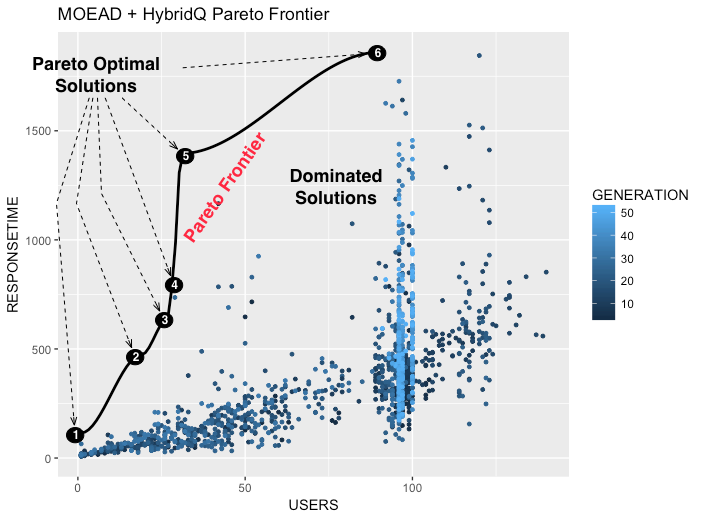
\includegraphics[width=1\textwidth]{./images/moeadhybridq.png}
    \caption{Collaborative approach Pareto Frontier}
\label{fig:singlewithmulti}
\end{figure}

\subsection{Experiment Research Questions}

The following research question is addressed:
\begin{itemize}
\item The combined use of MOEA/D with Hybrid could improve the results obtained in the previous experiments with MOEA/D?
\end{itemize}


\subsection{Variables}

The independent variable is the collaborative approach of the algorithms HybridQ and MOEA/D. The dependent variable is the hypervolume found by the new approach.

\subsection{Experiment Hypotheses}

\begin{itemize}
\item With regard to hypervolume:
\begin{itemize}
\item $H_{0}$ (null hypothesis): The hypervolume of the new approach don't surpass the previous experiments.
\item $H_{1}$: The hypervolume of the new approach surpass the previous experiments.
\end{itemize}
\end{itemize}


\subsection{Experiment Results}

At the end of 28 generations, the new approach obtains a hypervolume value of the 10.29. The new approach obtains a hypervolume of 10.84 at the end of 50 generations. Table \ref{tab:results2} and \ref{fig:singlewithmulti} presents 6 workloads that which are the Pareto optimal solution in the experiment. The algorithm found a workload with 31 users and response time of 1396, above the expected response time of 1000 milliseconds.

\subsection{Experiment Conclusion}

The results presented by the MOEA/D with HybridQ surpass previous approaches for the same number of generations.


% Please add the following required packages to your document preamble:
% \usepackage[table,xcdraw]{xcolor}
% If you use beamer only pass "xcolor=table" option, i.e. \documentclass[xcolor=table]{beamer}
\begin{table}[!h]
\centering
\caption{Response time and number of users in optimal scenarios found with MOEA/D + HybridQ}
\label{tab:results2}
\begin{tabular}{|l|l|l|l|l|l|l|l|l|}
\hline
\rowcolor[HTML]{C0C0C0}
\textbf{N.} & \textbf{\begin{tabular}[c]{@{}l@{}}USERS\\ \end{tabular}} & \textbf{\begin{tabular}[c]{@{}l@{}}RESP \\ TIME\end{tabular}} & \multicolumn{1}{c|}{\cellcolor[HTML]{C0C0C0}\textbf{\begin{tabular}[c]{@{}c@{}}Dogs\\ Users\end{tabular}}} & \textbf{\begin{tabular}[c]{@{}l@{}}Enter\\ Catalog\\ Users\end{tabular}} & \textbf{\begin{tabular}[c]{@{}l@{}}Fish\\ Users\end{tabular}} & \textbf{\begin{tabular}[c]{@{}l@{}}Register\\ Users\end{tabular}} & \textbf{\begin{tabular}[c]{@{}l@{}}Add\\ Rem.\\ Cart\end{tabular}} & \textbf{\begin{tabular}[c]{@{}l@{}}Cart\\ Users\end{tabular}} \\ \hline
\ding{202}           & 1                                                        & 115                                                        &                                                           &                                                                  &               &                   &                                                                    1 &               \\ \hline
\ding{203}           & 19                                                       & 473                                                        & 6                                                         &                                                                & 5             &               4   &                                                                    4 &               \\ \hline
\ding{204}          & 27                                                      & 644                                                        & 17                                                         &                                                                &         3      &                   &                                                                    & 7             \\ \hline
\ding{205}           & 28                                                      & 774                                                        &                                                          & 8                                                                &    3          & 3                 &                                                                   8 &     6          \\ \hline
\ding{206}           & 31                                                      & 1396                                                       & 6                                                          &                                                                &              &    13             & 4                                                                   & 8               \\ \hline
\ding{207}           & 90                                                     & 1860                                                        & 12                                                          & 11                                                              & 3             &        3          & 30                                                                  &   31            \\ \hline
\end{tabular}
\end{table}

\section{Analysis of Pareto Frontier  in Multiple Executions}

Due to the pervasive and non-deterministic nature of the problem, there is no guarantee that the same Pareto frontier will be found in different test executions. This section provides an initial study to evaluate the Pareto frontier difference in multiple executions. The experiment was conducted with the JPetStore application with the SEDR adapted  noise reduction strategy. The maximum tolerated response time in the test was 1000 milliseconds.  The whole process of stress  tests, which run for 2 days and 983 executions. The tool automatically selected the next scenarios to be run up to the limit of 23 previously established  generations by the algorithm. Three executions were carried out with different initial populations. Figs. \ref{fig:comp1} and \ref{fig:comp2} presents the comparative results between the three executions (1, 2 and 3).

\subsection{Experiment Research Questions}

The following research question is addressed:
\begin{itemize}
\item There is an acceptable variation of the Pareto frontier for the three test executions?
\end{itemize}


\subsection{Variables}

The independent variable is three test executions using the collaborative approach with the algorithms HybridQ and MOEA/D. The dependent variable is the hypervolume and Pareto frontier found by each test execution.

\begin{figure}[h]
\centering
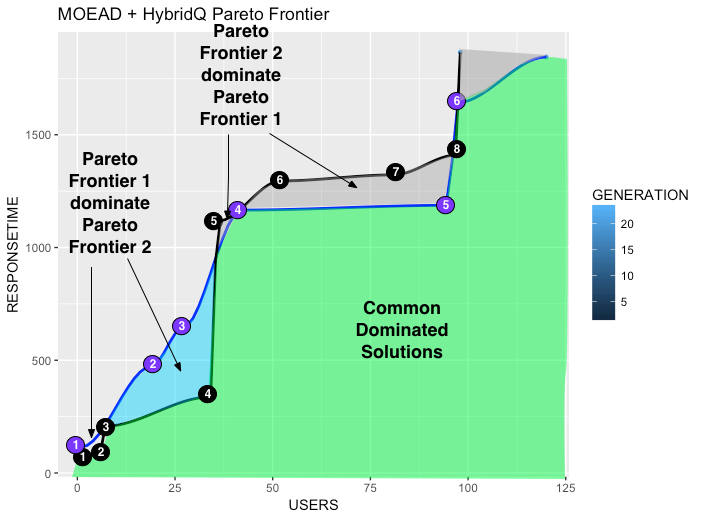
\includegraphics[width=1\textwidth]{./images/comparative.png}
    \caption{Pareto Frontier of the first and second test executions}
\label{fig:comp1}
\end{figure}


\begin{figure}[h]
\centering
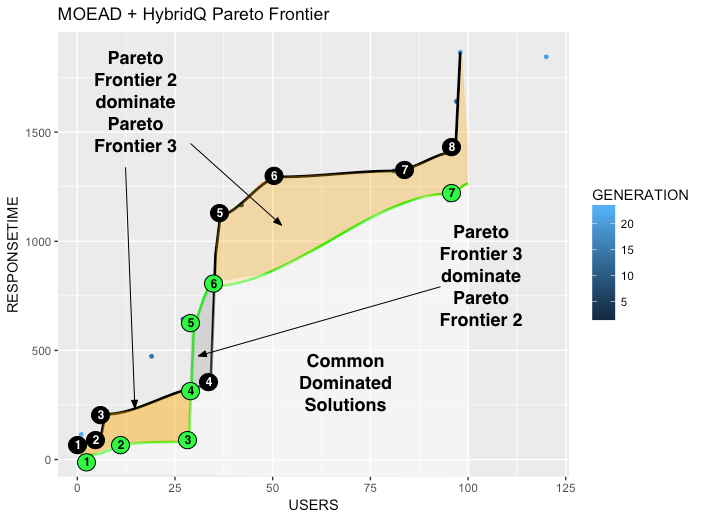
\includegraphics[width=1\textwidth]{./images/comparative2.png}
    \caption{Pareto Frontier of the second and third test executions}
\label{fig:comp2}
\end{figure}

\subsection{Experiment Hypotheses}


\begin{itemize}
\item $H_{0}$  (null hypothesis): The hypervolume variation of the three tests performed is greater than 10\%.
\item $H_{1}$: The hypervolume variation of the three tests performed is less than 10\%.
\end{itemize}


\subsection{Experiment Results}

Table \ref{tab:results2} presents the experiment results. The variation between stayed around 17\%. Further studies are needed to ascertain more accurately the variation of the Pareto frontier.

% Please add the following required packages to your document preamble:
% \usepackage[table,xcdraw]{xcolor}
% If you use beamer only pass "xcolor=table" option, i.e. \documentclass[xcolor=table]{beamer}
\begin{table}[]
\centering
\caption{Experiment Results}
\label{my-label}
\begin{tabular}{|l|l|ll}
\cline{1-2}
\cellcolor[HTML]{EFEFEF}\textbf{Test Execution} & \cellcolor[HTML]{EFEFEF}\textbf{Hypervolume} &                                                     &                                        \\ \hline
1                                               & 9.377189                                     & \multicolumn{1}{l|}{\textbf{Average}}               & \multicolumn{1}{l|}{8.652338}          \\ \hline
2                                               & 9.648418                                     & \multicolumn{1}{l|}{\textbf{Standard Deviation}}   & \multicolumn{1}{l|}{1.49652728764998}  \\ \hline
3                                               & 6.931407                                     & \multicolumn{1}{l|}{\textbf{Percent deviation}} & \multicolumn{1}{l|}{0.172962185209359} \\ \hline
\end{tabular}
\end{table}


\section{Conclusion}


The use of multi-objective metaheuristics has made it possible to delimit a frontier where the response times are below the previously established service level. MOEA/D metaheuristics obtained the best hypervolume value when compared with NSGA II, SPEA2 and PAES. The MOEA / D algorithm dominates most of the results presented by HybridQ. However, we have verified from the experiments that some of the results found by the HybridQ algorithm can contribute to the use of MOEA/D. Thus, we propose the collaborative use of  MOEA/D and HybridQ algorithms.  The collaborative approach improves the hypervolume values obtained and found more relevant workloads than the previous experiments. 

For the time being, we cannot state that the benefits found by using MOEA / D and HybridQ algorithms together can be obtained in other contexts. Due to the pervasive and non-deterministic nature of the problem, we do not guarantee that the same Pareto frontier will be found in different test executions.  More experiments are needed to verify changes related to the Pareto frontier in different executions.


% conference papers do not normally have an appendix

% use section* for acknowledgment






% trigger a \newpage just before the given reference
% number - used to balance the columns on the last page
% adjust value as needed - may need to be readjusted if
% the document is modified later
%\IEEEtriggeratref{8}
% The "triggered" command can be changed if desired:
%\IEEEtriggercmd{\enlargethispage{-5in}}

% references section

% can use a bibliography generated by BibTeX as a .bbl file
% BibTeX documentation can be easily obtained at:
% http://mirror.ctan.org/biblio/bibtex/contrib/doc/
% The IEEEtran BibTeX style support page is at:
% http://www.michaelshell.org/tex/ieeetran/bibtex/
%\bibliographystyle{IEEEtran}
% argument is your BibTeX string definitions and bibliography database(s)
%\bibliography{IEEEabrv,../bib/paper}
%
% <OR> manually copy in the resultant .bbl file
% set second argument of \begin to the number of references
% (used to reserve space for the reference number labels box)
\chapter{Conclusion}

This chapter presents our conclusions, revisits the contributions, shows some limitations, and proposals for future work. In this thesis, we deal with the use of hybrid metaheuristics, reinforcement learning and multi-objective metaheuristics in Search-based stress testing. A tool named IAdapter, a JMeter plugin for performing search-based load tests, was developed. Several experiments were conducted to validate the proposed approach.

\section{Summary of contributions and Achievements}

First, we proposed a hybrid collaborative algorithm to perform search-based stress testing. In order to enhance the efficiency of our proposal, we utilize the reinforcement learning technique with the aforementioned hybrid algorithm. We also proposed the use of multi-objective algorithms in search-based stress testing. To this end, we propose an adaptation of the SEDR algorithm for noise reduction and a new approach to the use of a multiobjective metaheuristic in conjunction with the HybridQ algorithm. We conduct numerous experiments to evaluate the proposed approaches. The use of multi-objective metaheuristics has made it possible to delimit a frontier where the response times are below the previously established service level. The subsequent subsections present the summary of results for each research question.

\textbf{(Research Question 1) How to improve the search for test scenarios in search-based stress testing using single-objective metaheuristics?}


The hybrid approach uses genetic algorithms, tabu search, and simulated annealing. Three experiments were performed to validate the hybrid metaheuristic. The first experiment aimed to execute stress testing on a simulated component. In the first experiment, the signed-rank Wilcoxon non-parametrical procedure was used for comparing the results. The procedure showed that there was a significant improvement in  results with the Hybrid Metaheuristic approach when compared with the other algorithms. All tests in the experiment were conducted without the need of a tester, automating  stress testing with the JMeter tool \cite{Gois2016}. 



\textbf{(Research Question 2) How to improve the choice of neighboring solutions in a single-objective metaheuristic to explore, reducing the time needed to obtain the scenarios with the longest response time in the application?}


The HybridQ algorithm is used to optimize the choice of neighboring solutions to explore, reducing the time needed to obtain the scenarios with the longest response time in the application. The research assumes that HybridQ is more expensive than Hybrid because of Q-learning. The research has as the premise that the same application under performance tests can be submitted to more than one cycle of tests execution, decreasing the cost of the exploration phase of the Q-learning algorithm used. HybridQ algorithm obtains the maximum value of fitness, but it needs a much greater number of requests than the other algorithms. GA was the algorithm that obtains the best fitness value with a minor number of requests. 


\textbf{(Research Question 3) How to use multi-objective metaheuristics in search-based stress testing to obtain a Pareto frontier to improve the definition of SLAs?}

The experiment with NSGA-II algorithm discovers application scenarios where there is a high response time for a small number of users. The experiment found 8 optimal workloads that present a lower number of users with high response times. The results of the experiment can help in the decision making of service levels that need to be defined for the application \cite{Gois2017}. MOEA/D metaheuristics obtained the best hypervolume value when compared with NSGA II, SPEA2 and PAES. The MOEA/D algorithm dominates most of the results presented by HybridQ. However, we have verified from the experiments that some of the results found by the HybridQ algorithm can contribute to the use of MOEA/D. The collaborative approach (HybridQ+MOEA/D) improves the hypervolume values obtained and found more relevant workloads than the previous experiments. The experiments found  scenarios that contribute to the definition of the service level. To take an example, the second experiment with the hybrid algorithm found scenarios with only 35 users but which already have a response time greater than the maximum defined for the service level.

\section{Future Works and Open Issues}

There is a range of future improvements in the proposed approach. Also as a typical search strategy, it is sometimes difficult to ensure that the execution times generated in the experiments represent global optimum. More experimentation is also required to determine the most appropriate and robust parameters. Lastly, there is necessary to have an adequate termination criterion to stop the search process. 

More experiments are needed to state that the benefits found by using MOEA/D and HybridQ algorithms together can be obtained in other contexts.  More experiments are needed in order to verify changes related to the Pareto frontier in different executions.

The choice of fitness function can be a difficult step in Genetic Algorithms. Different fitness functions promote different GA behavior. The fitness function is still manually adjusted and additional studies need to be performed to get the best weight values for the fitness function. There is a great difficulty in
comparing some approaches present in the state-of-art, due to the lack of availability of the tools used. The present research compared the proposed approach with other methods based on the use of single or multiobjective metaheuristics.


Among the future works of the research, the use of different combinatorial optimization algorithms such as very large-scale neighborhood search is one that we can highlight. Further research should ascertain more exhaustively the variation of the Pareto frontier. Further experiments with reinforcement learning in conjunction with multi-objective search algorithms must be performed. The PAES algorithm performs a local search is can be benefited with the strategies outlined in this research. Additional experiments are needed to see if the benefits found by this thesis in the context of stress testing will be obtained in other contexts.



\appendix


\bibliographystyle{abnt-alf}
\bibliography{bibliografia}

\chapter{Stress Testing}


This chapter surveys the state of the art literature in stress testing research. The thesis extends the survey presented by Jiang et al. \cite{Jiang2010}  and Afzal et al. \cite{Afzal2009a} to the Stress Testing context.  This survey will be helpful for stress testing practitioners and software engineering researchers with interests in testing and analyzing software systems. The paper uses the systematic review method proposed by Kitchenham \cite{Kitchenham2007}. The systematic review is based on a comprehensive set of 97 articles obtained after a multi-stage selection process and have been published in the time span 1994–2016.

\section{Research Questions}

In order to examine the evidence of stress testing properties, we proposed the following two research questions:


\begin{itemize}
\item How modeling a stress test workload?
\item What are the main anti-patterns found by stress tests?
\end{itemize}


\subsection{Study Selection Criteria}

The population in this study is the domain of software testing. Intervention includes the application of stress test techniques to test different types of non-functional properties. The primary studies used in this review were obtained from
searching databases of peer-reviewed software engineering research that met the following criteria: contains peer-reviewed software engineering journals articles, conference proceedings, and book chapters; contains multiple journals and conference proceedings,
which include volumes that range from 1996 to 2017.

The resulting list of databases was:

\begin{itemize}
\item  ACM Digital Library
\item  Google Scholar
\item  IEEE Electronic Library
\item  Inspec
\item  Scirus (Elsevier)
\item SpringerLink
\end{itemize}


The search strategy was based on the following steps:  Identification of alternate words and synonyms for terms used
in the research questions. This is done to minimize the effect
of differences in terminologies. Identify common stress testing properties for searching.  Use of Boolean OR to join alternate words and synonyms and use of Boolean AND to join major terms.

We used the following search terms:

\begin{itemize}
\item Load Testing: load test, Load Testing
\item Stress Testing: stress test, stress testing
\item Performance Testing: Performance tests
\item Test tools: JMeter, load runner, performance tester
\end{itemize}



The idealized selection process was done in two parts: an initial document selection of the results that could reasonably satisfy the selection criteria based on a title and the articles abstract reading, followed by a final selection of the initially selected papers based on the introduction and conclusion reading of the papers. The following exclusion criteria are applicable in this review, i.e. exclude studies that:
\begin{itemize}
\item Do not relate to stress testing.
\item Do not relate to load testing tool.
\item Do not relate to load/stress testing model.
\end{itemize}

From 366 initial papers, 97 papers were selected.

\section{Stress Test Process}

Contrary to functional testing, which has clear testing objectives, Stress testing objectives are not clear in the early development stages and are often defined later on a case-by-case basis. The Fig. \ref{fig:testprocess} shows a common Load, Performance and Stress test process  \cite{Jiang2010}.

\begin{figure}[!ht]
\centering
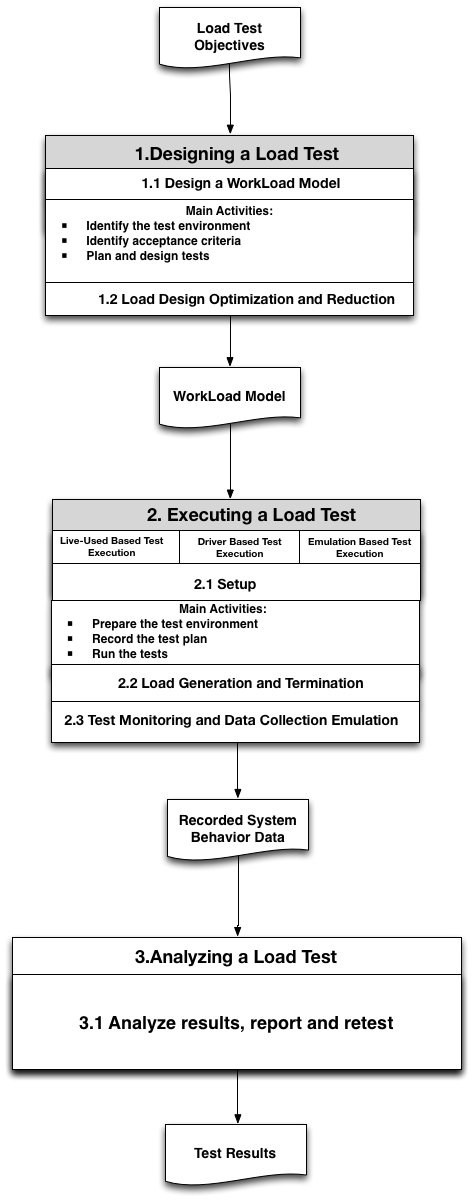
\includegraphics[width=0.4\textwidth]{./images/testprocess.png}
\caption{Load, Performance and Stress Test Process \cite{Jiang2010}\cite{Erinle2013}}
\label{fig:testprocess}
\end{figure}


The goal of the load design phase is to devise a load, which can uncover non-functional problems. Once the load is defined, the system under test executes the load and the system behavior under load are recorded. Load testing practitioners then analyze the system behavior to detect problems \cite{Jiang2010}.

Once a proper load is designed, a load test is executed. The load test execution phase consists of the following three main aspects: (1) Setup, which includes system deployment and test execution setup; (2) Load Generation and Termination, which consists of generating the load; and (3) Test Monitoring and Data Collection, which includes recording the system behavior during execution\cite{Jiang2010}.

The core activities in conducting a usual Load, Performance and Stress tests are \cite{Erinle2013}:

\begin{itemize}
\item Identify the test environment: identify test and production environments and knowing the hardware, software, and network configurations help derive an effective test plan and identify testing challenges from the outset.

\item Identify acceptance criteria: identify the response time, throughput, and resource utilization goals and constraints.

\item Plan and design tests: identify the test scenarios.In the context of testing, a scenario is a sequence of steps in an application. It can represent a use case or a business function such as searching a product catalog, adding an item to a shopping cart, or placing an order \cite{Corporation2007}. This task includes a description
of the speed, availability, data volume throughput rate, response
time, and recovery time of various functions, stress, and so on. This
serves as a basis for understanding the level of performance and
stress testing that may be required to each test scenario \cite{Lewis2005}.

\item Prepare the test environment: configure the test environment, tools, and resources necessary to conduct the planned test scenarios.

\item Record the test plan: record the planned test scenarios using a testing tool.

\item Run the tests: Once recorded, execute the test plans under light load and verify the correctness of the test scripts and output results.

\item Analyze results, report, and retest: examine the results of each successive run and identify areas of bottleneck that need addressing.

\end{itemize}

Utting et al. presents four classic test process \cite{utting2010practical}: 

\begin{itemize}
\item Manual Testing process;
\item Capture/Replay Testing process; 
\item Script-based Testing process;
\item Keyword-Driven Automated Testing process;

\end{itemize}

In a Manual Testing process, the execution is done manually for each test case. The tester follows a test case and interacts directly with the application under test. The manual-designing of the tests is time-consuming and not ensure systematic coverage of the application. Capture/Replay attempts to reduce the cost of test re-execution by capturing interactions with the application during a test execution session and replay those interactions in later test executions \cite{utting2010practical}.

A test script is an executable script that runs one or more test cases. The Script-based testing process tries to resolve the test execution problem by automating it. Keyword-driven testing, or action-word testing, takes this a step further by using action keywords in the test cases, in addition to data. Each action keyword corresponds to a fragment of a test script \cite{utting2010practical}.


\section{Stress Test Execution}

The stress test execution consists of deploying the system and setup test execution; generating workloads according to the configurations and terminating the load when the load test is completed and recording the system behavior. There are three general approaches of load test executions \cite{Molyneaux2009}\cite{Jiang2010}:

\begin{itemize}
\item Live-User Based Executions: The test examines a system’s behavior when the system is simultaneously used by many users or execute a load test by employing a group of human testers.
\item Driver Based Executions: The driver based execution approach automatically generate thousands or millions of concurrent requests for a long period of time using a software tool.
\item Emulation Based Executions: The emulation based load test execution approach performs the load testing on special platforms and doesn't require a fully functional system and conduct load testing.
\end{itemize}

Usually, a stress test execution it is performed with Driver Based Executions approaches \cite{Erinle2013} \cite{MohammadS.Obaidat} \cite{Wang2013}. There are three categories of load drivers \cite{Jiang2010}:

\begin{itemize}
\item Benchmark Suite: specialized load driver, designed for one type of system. For example, LoadGen is a load driver specified used to load test the Microsoft Exchange MailServer.
\item  Centralized Load Drivers: refer to a single load driver, which generates the load.
\item Peer-to-peer Load Drivers: refer to a set of load drivers, which collectively generate the target testing load. Peer-to-peer load drivers usually have a controller component, which coordinates the load generation among the peer load drivers.
\end{itemize}

A stress test needs to perform hundreds or thousands of concurrent requests to the application under test. Automated tools are needed to carry out serious load, stress, and performance testing. Sometimes, there is simply no practical way to provide reliable, repeatable performance tests without using some form of automation. The aim of any automated test tool is to simplify the testing process.


\subsection{Stress Testing Tools}

There are several tools to the execution of stress testing. Stress testing tools are software products based on workload models to generate request sequences similar to real requests. They are designed and implemented as versatile software tools for performing tuning or capacity planning studies. Usually, the tool functions are semi-automated, whereas the execution of the tests itself is performed by a tool, the choice of scenarios to be executed as well as the decision to start new execution batteries are activities of the test designer or tester. Normally, load test tools use test scripts. Test scripts are written in a GUI testing framework or a back-end server-directed performance tool such as JMeter. These frameworks are the basis on which performance testing is mostly done in industry. Performance test scripts imitate large numbers of users to create a significant load on the application under tests. Stress testing tools typically have the following components \cite{Grechanik2012} \cite{Molyneaux2009}:

\begin{itemize}
\item Scripting module: Enable recording of end-user activities in different middleware protocols;
\item Test management module: Allows the creation of test scenarios;
\item Load injectors: Generate the load with multiple workstations or servers;
\item Analysis module Provides the ability to analyze the data collected by each test iteration.
\end{itemize}


Comparing stress test tools is a laborious and difficult task since they offer a large amount and diversity of features \cite{Dustin1999}. In next subsection we present studies that contrast stress testing tools according to a wide set of features and capabilities, focusing on their ability to realize search-based tests or have learning capacities. In the following subsection, we present details about the JMeter tool and the reasons why it was chosen as the object of the present research.The stress test tools were categorized in three different groups \cite{MohammadS.Obaidat}:

\begin{itemize}
\item Benchmarks that model the client and server paradigm in the Web context.
\item Software products to evaluate performance and functionality of a given Web application, such as LoadRunner, WebLOAD, and JMeter.
\item Testing tools and other approaches for traffic generation based on HTTP traces.
\end{itemize}

\subsection{Comparative Studies}

Illes et al. present a systematic approach for evaluation criteria for test tools. Using the TORE methodology the study identify activities which potentially could be automated or at least supported by a test tool. The study evaluates three tools: WinRunner, Rational Robot and HTTrace. WinRunner is distributed by Mercury.  an. HTTrace is not a commercial product but developed for internal use for the company i-TV-T. The study evaluates the tools in the tasks: TestPlanning and monitoring, designing test cases, constructing test cases, executing test cases and analyzing test cases. Key features of all three test tools are the construction of test cases by
capturing and subsequently editing the test scripts and the execution of the recorded test
scripts.  WinRunner and Rational Robot can be extended to provide test planning and monitoring as well as defect and reporting facilities. HTTrace’s strength lies on testing database applications by allowing the reset of consistent database states. Additionally, all three tools can be extended to provide support for testing quality attributes of the system under test \cite{Illes2005}.

Tables \ref{tab: tabtool1} and \ref{tab: tabtool2} summarizes the studied workloads generators as well as the grade (full or partial) in which they fulfill the features described below. None of the presented tools uses heuristic or learning resources when choosing the scenarios to be tested or the workloads to be applied in the test.

Penã-Ortiz et al. present a study where stress test tools are compared using 12 features \cite{MohammadS.Obaidat}:

\begin{itemize}
\item Distributed architecture. This refers to the ability to distribute the generation process among different nodes.
\item Analytical-based architecture. This feature represents the capability to use analytical and mathematical models to define the workload.
\item Business-based architecture. When defining a testing environment, the simulator architecture should implement the same features as the real environment.
\item Client parameterization. This is the ability to parameterize generator nodes.
\item Workload types. Some generators organize the workload in categories or types.
\item Testing the Web application functionality (functional testing).
\item Multi-platform refers to a software package that is implemented in multiple types of computer platforms, inter-operating among them.
\item Differences between LAN and WAN.
\item The generator should be a friendly application.
\item The load test tool has performance reports.
\item The load test tool is open-source.
\item Users’ dynamism. The users have the ability of change the behavior in during the test.
\end{itemize}


% Please add the following required packages to your document preamble:
% \usepackage[table,xcdraw]{xcolor}
% If you use beamer only pass "xcolor=table" option, i.e. \documentclass[xcolor=table]{beamer}
\begin{table}[]
\centering
\caption{Benchmarks group}
\label{tab: tabtool1}
\begin{tabular}{|l|l|l|l|l|l|}
\hline
\rowcolor[HTML]{EFEFEF}
\textbf{Feature/Tool}         & \textbf{WebStone} & \textbf{SpecWeb} & \textbf{SURGE} & \textbf{Web Polygraph} & \textbf{TPC-W} \\ \hline
\cellcolor[HTML]{EFEFEF} \begin{minipage}{0.2\textwidth} Analytical-Based\\ Architecture \\ \end{minipage} & Full sup.      & Full sup.     & Full sup.   & Full sup.           & Full sup.   \\ \hline
\cellcolor[HTML]{EFEFEF}\begin{minipage}{0.2\textwidth}Distributed\\ Architecture \\   \end{minipage}    & Full sup.      & Full sup.     & Full sup.   & Full sup.           &                \\ \hline
\cellcolor[HTML]{EFEFEF}\begin{minipage}{0.2\textwidth}Business-Based Architecture \\ \end{minipage}  &                   & Partial Support   &                & Partial Support         & Full sup.   \\ \hline
\cellcolor[HTML]{EFEFEF}\begin{minipage}{0.2\textwidth}Client\\ Parameterization \\\end{minipage}       & Full sup.      & Full sup.     &                & Partial Support         & Full sup.   \\ \hline
\cellcolor[HTML]{EFEFEF}Workload Types                &                   & Full sup.     &                &                        & Full sup.   \\ \hline
\cellcolor[HTML]{EFEFEF}Functional Testing            &                   &                  &                &                        &                \\ \hline
\cellcolor[HTML]{EFEFEF}LAN and WAN                   &                   &                  &                &                        &                \\ \hline
\cellcolor[HTML]{EFEFEF}Multi-platform                & Full sup.      & Full sup.     & Full sup.   & Full sup.           & Full sup.   \\ \hline
\cellcolor[HTML]{EFEFEF}Ease of Use                   &                   &                  &                &                        &                \\ \hline
\cellcolor[HTML]{EFEFEF}\begin{minipage}{0.2\textwidth}Performance Reports\end{minipage}           & Partial Support    & Full sup.     &                & Full sup.           & Full sup.   \\ \hline
\cellcolor[HTML]{EFEFEF}Open Source                   & Full sup.      &                  & Full sup.   & Partial Support         & Full sup.   \\ \hline
\cellcolor[HTML]{EFEFEF}User’s Dynamism               &                   &                  &                &                        & Partial Support \\ \hline
\end{tabular}
\end{table}


% Please add the following required packages to your document preamble:
% \usepackage[table,xcdraw]{xcolor}
% If you use beamer only pass "xcolor=table" option, i.e. \documentclass[xcolor=table]{beamer}
\begin{table}[h]
\centering
\caption{Software products}
\label{tab: tabtool2}
\begin{tabular}{|l|l|l|l|}
\hline
\rowcolor[HTML]{EFEFEF}
\textbf{Feature/Tool}         & \textbf{LoadRunner} & \textbf{WebLOAD} & \textbf{JMeter} \\ \hline
\cellcolor[HTML]{EFEFEF}Analytical-Based Architecture & Partial Support      & Partial Support   & Partial Support  \\ \hline
\cellcolor[HTML]{EFEFEF}Distributed Architecture      & Full support        & Full support     & Full support    \\ \hline
\cellcolor[HTML]{EFEFEF}Business-Based Architecture   & Full support        & Full support     & Full support    \\ \hline
\cellcolor[HTML]{EFEFEF}Client Parameterization       & Full support        & Full support     & Full support    \\ \hline
\cellcolor[HTML]{EFEFEF}Workload Types                & Full support        & Full support     & Partial Support  \\ \hline
\cellcolor[HTML]{EFEFEF}Functional Testing            & Full support        & Full support     & Partial Support  \\ \hline
\cellcolor[HTML]{EFEFEF}LAN and WAN                   &                     &                  &                 \\ \hline
\cellcolor[HTML]{EFEFEF}Multi-platform                & Full support        & Full support     & Full support    \\ \hline
\cellcolor[HTML]{EFEFEF}Ease of Use                   & Full support        & Full support     & Partial Support  \\ \hline
\cellcolor[HTML]{EFEFEF}Performance Reports           & Partial Support      & Full support     & Full support    \\ \hline
\cellcolor[HTML]{EFEFEF}Open Source                   &                     &                  & Partial Support  \\ \hline
\cellcolor[HTML]{EFEFEF}User’s Dynamism               & Partial Support      & Partial Support   & Partial Support  \\ \hline
\end{tabular}
\end{table}

\subsection{Benchmarks Group}

WebStone was designed by Silicon Graphics in 1996 to measure the performance of Web server software and hardware products. Nowadays, both executable and source actualized code for WebStone are available for free. The benchmark generates a Web server load by simulating multiple Web clients navigating a website. All the testing done by the benchmark is controlled by a Webmaster, which is a program that can be run on one of the client computers or on a different one \cite{MohammadS.Obaidat} \cite{Trent1995} .

TPC Benchmark (TPC-W) is a transitional Web benchmark defined by the Transaction Processing Performance Council that models a representative e-commerce evaluating the architecture performance on a generic profile.The models use a remote browser emulator to generate requests to the server under test. TPC-W adopts the CBMG model to define the workloads in spite of this model only characterizing user dynamic behavior partially. The remote browser emulators are located on the client side and generate workload towards the e-commerce Web application, which is located on the server side (e-commerce server) \cite{MohammadS.Obaidat} \cite{Menasce2002a}.

\begin{figure}[h]
\centering
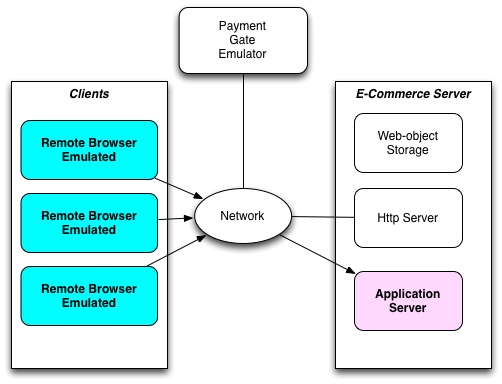
\includegraphics[width=0.6\textwidth]{./images/tpcw.png}
\caption{TPC-W architecture \cite{MohammadS.Obaidat} \cite{Menasce2002a}}
\label{fig:tpcw}
\end{figure}


Open STA is an open source software developed in C++ and released under the GPL license. OpenSTA provides a scripting language which permits to simulate the activity of a user. This language can describe HTTP/S scenario and all the test executions is managed in a graphical interface. The composition of the test is
very simple, allowing the tester choose scripts for a test and a remote computer that will execute each test.

\subsection{Software Products}

LoadRunner is one of the most popular industry-standard software products for functional and performance testing. It was originally developed by Mercury Interactive, but nowadays it is commercialized by Hewlett-Packard. LoadRunner supports the definition of user navigation, which is represented using a scripting language. The basic steps are recorded, creating a shell script. Next, this script is then taken off-line and undergoes further manual steps such as data parameterization and correlations. Finally, the desired performance scripts are obtained after adding transactions and any other required logic (Fig. \ref{fig:loadrunner}). LoadRunner scripting only permits partial reproduction of user dynamism when generating Web workload, because it cannot define either advanced interactions of users, such as parallel browsing behavior, or continuous changes in user’s behaviors \cite{MohammadS.Obaidat}.

\begin{figure}[!ht]
\centering
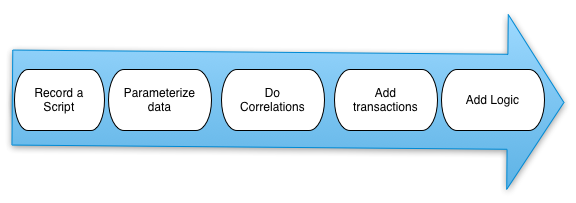
\includegraphics[width=0.6\textwidth]{./images/loadrunner.png}
\caption{Load Runner Scripting}
\label{fig:loadrunner}
\end{figure}



WebLOAD is a software tool for Web performance commercialized by RadView. It is oriented to explore the performance of critical Web applications by quantifying the utilization of the main server resources. The tool creates scenarios that try to mimic the navigation of real users. To this end, it provides facilities to record, edit and debug test scripts, which are used to define the scenarios on workload characterization. The execution environment is a console to manage test execution, whose results are analyzed in the Analytics application. Since WebLOAD is a distributed system, it is possible to deploy several load generators to reproduce the desired load. Load generators can also be used as probing clients where a single virtual user is simulated to evaluate specific statistics of a single user. These probing clients resemble the experience of a real user using the system while it is under load \cite{MohammadS.Obaidat}.

\subsection{Cloud Testing Tools}

Nachiyappan and Justus show a set of other tools perform Cloud testing. Cloud testing is a form of evaluation methodology in which the applications to be tested uses the cloud as a computing environment and its infrastructure to simulate real world traffic by using existing cloud computing technologies. Cloud testing is challenged by several problems such as limited budget, meeting deadlines, High cost per test, a large number of test cases, little reuse of tests and geographical distributions of users.  Blitz is a load-testing tool from the cloud to the cloud. Blitz has no client to install and it is unable to test applications behind firewalls or otherwise protected from the Internet. Blaze Meter is a cloud application based on JMeter scripts that allow stress and load tests on the cloud \cite{Nachiyappan2015}.

SOASTA CloudTest is a production performance testing
tool for Web applications. It can simulate thousands of virtual users visiting website simultaneously, using either private or public cloud infrastructure service. The worker nodes can be distributed across public and private clouds to cooperate in a large load testing. Test results from distributed test agents are
integrated for analysis \cite{Bai2011a}.

\subsection{Apache JMeter}

Apache JMeter was the tool chosen for current research due to its open license, the use of plugins and the ease of integration with jmetal and jgap frameworks. Apache JMeter is a free open source stress testing tool.  It has a large user base and offers lots of plugins to aid testing. JMeter is a desktop application designed to test and measure the performance and functional behavior of applications. The application it is purely Java-based and is highly extensible through a provided API (Application Programming Interface). JMeter works by acting as the client of a client/server application. JMeter allows multiple concurrent users to be simulated on the application \cite{Halili2008} \cite{Erinle2013}.

Apache JMeter is used to generate heavy loads on the servers or objects to test its strength or analyze overall performance under different load types. To briefly explain the solution how it works, as follows: A Regular Expression Extractor captures the dynamic values as mentioned above and stored in a temporary variable. The values which have been extracted and stored in temporary variables are subsequently utilized by immediate requests/re directions using HTTP samplers \cite{Kiran2015}. JMeter has components organized in a hierarchical manner. The Test Plan is the main component in a JMeter script. A typical test plan will consist of one or more Thread Groups, logic controllers, listeners, timers, assertions, and configuration elements:

\begin{itemize}
\item Thread Group: Test management module responsible for emulating the users used in a test. All elements of a test plan must be under a thread group.
\item Listeners: Analysis module responsible for providing access to the information gathered by JMeter about the test cases.
\item Samplers: Load injectors module responsible for sending requests to a server, while Logical Controllers let you customize its logic.
\item Timers: allow JMeter to delay between each request.
\item Assertions: test if the application under test it is returning the correct results.
\item Configuration Elements: configure details about the request protocol and test elements.
\end{itemize}


\FloatBarrier

\section{Research Question 1: How to  model a stress test workload?}


The design of a stress test depends intrinsically on the load model applied to the software under test. Based on the objectives, there are two general schools of thought for designing a proper load to achieve such objectives \cite{Afzal2009a}:

\begin{itemize}
\item Designing Realistic Loads (Descriptive Workload).
\item Designing Fault-Inducing Loads (Generative Workload).
\end{itemize}

In Designing Realistic Loads, the main goal of testing is to ensure that the system can function correctly once. Designing Fault-Inducing Loads aims to design loads, which are likely to cause functional or non-functional problems \cite{Afzal2009a}.

Stress testing projects should start with the development of a model for user workload that an application receives. This should take into consideration various performance aspects of the application and the infrastructure that a given workload will impact. A workload is a key component of such a model \cite{Molyneaux2009}.

The term workload represents the size of the demand that will be imposed on the application under test in an execution. The metric used to measure a workload is dependent on the application domain, such as the length of the video in a transcoding application for multimedia files or the size of the input files in a file compression application \cite{Feitelson2013} \cite{Molyneaux2009} \cite{Goncalves2014}.

The workload is also defined by the load distribution between the identified transactions at a given time. Workload helps researchers study the system behavior identified in several load models. A workload model can be designed to verify the predictability, repeatability, and scalability of a system \cite{Feitelson2013} \cite{Molyneaux2009}. Workload modeling is the attempt to create a simple and generic model that can then be used to generate synthetic workloads. The goal is to create workloads that can be used in performance evaluation studies. Sometimes, the synthetic workload is supposed to be similar to those that occur in practice in real systems \cite{Feitelson2013} \cite{Molyneaux2009}.

There are two kinds of workload models: descriptive and generative. The main difference between the two is that descriptive models just try to mimic the phenomena observed in the workload, whereas generative models try to emulate the process that generated the workload in the first place \cite{Feitelson2013}.

In descriptive models, one finds different levels of abstraction on the one hand and different levels of fidelity to the original data on the other hand. The most strictly faithful models try to mimic the data directly using the statistical distribution of the data. The most common strategy used in descriptive modeling is to create a statistical model of an observed workload. This model is applied to all the workload attributes, e.g., computation, memory usage, I/O behavior, communication, etc. \cite{Feitelson2013}. Fig. \ref{fig:descriptivemodel} shows a simplified workflow of a descriptive model. The workflow has six phases. In the first phase, the user uses the system in the production environment. In the second phase, the tester collects the user's data, such as logs, clicks, and preferences, from the system. The third phase consists of developing a model designed to emulate the user's behavior. The fourth phase is made up of the execution of the test, emulation of the user's behavior, and log gathering.



\begin{figure}[!ht]

\centering
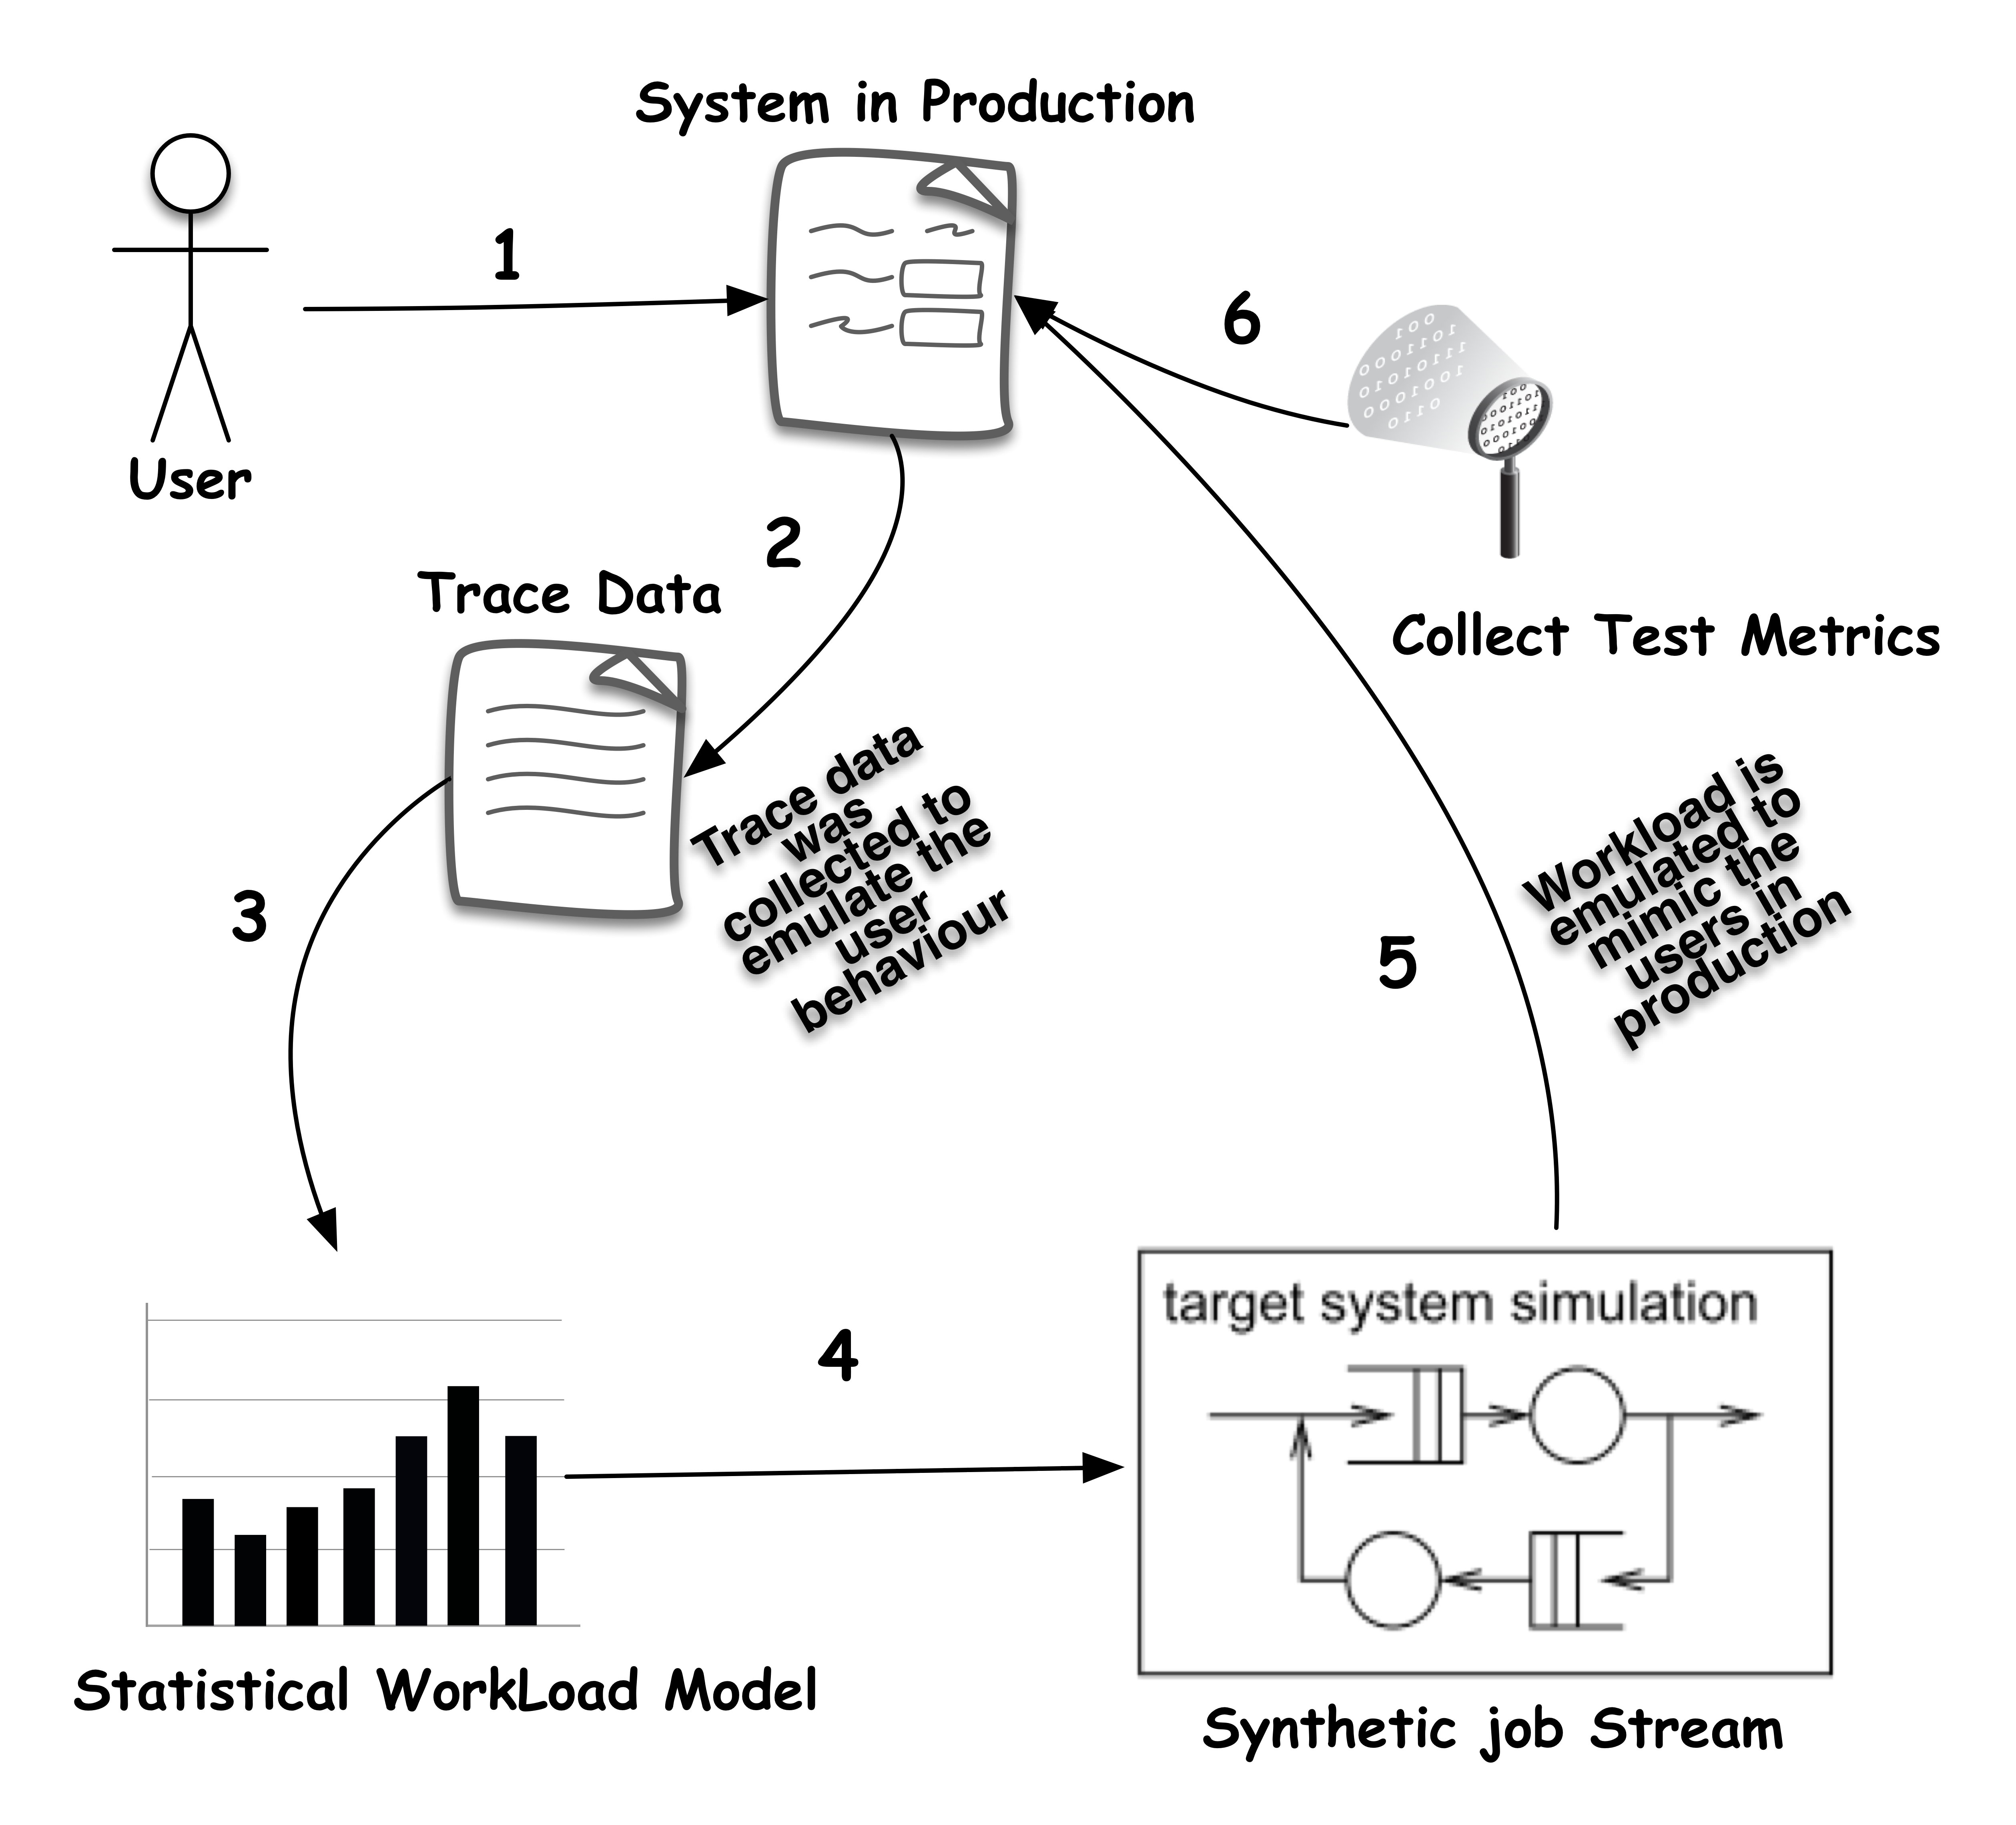
\includegraphics[width=0.6\textwidth]{./images/workloadmodel1300dpi.png}
\caption{Workload modeling based on statistical data \cite{DiLucca2006}}
\label{fig:descriptivemodel}
\end{figure}


Generative models are indirect in the sense that they do not model the statistical distributions. Instead, they describe how users will behave when they generate the workload. Consequently, an important benefit of the generative approach is that it facilitates manipulations of the workload. It is often desirable to be able to change the workload conditions as part of the evaluation. Descriptive models do not offer any option regarding how to do so. With the generative models, however, we can modify the workload-generation process to fit the desired conditions \cite{Feitelson2013}. The difference between the workflows of the descriptive and the generative models is that user behavior is not collected from logs but simulated from a model that can receive feedback from the test execution (Fig. \ref{fig:generativemodel}).


\begin{figure}[h]
\centering
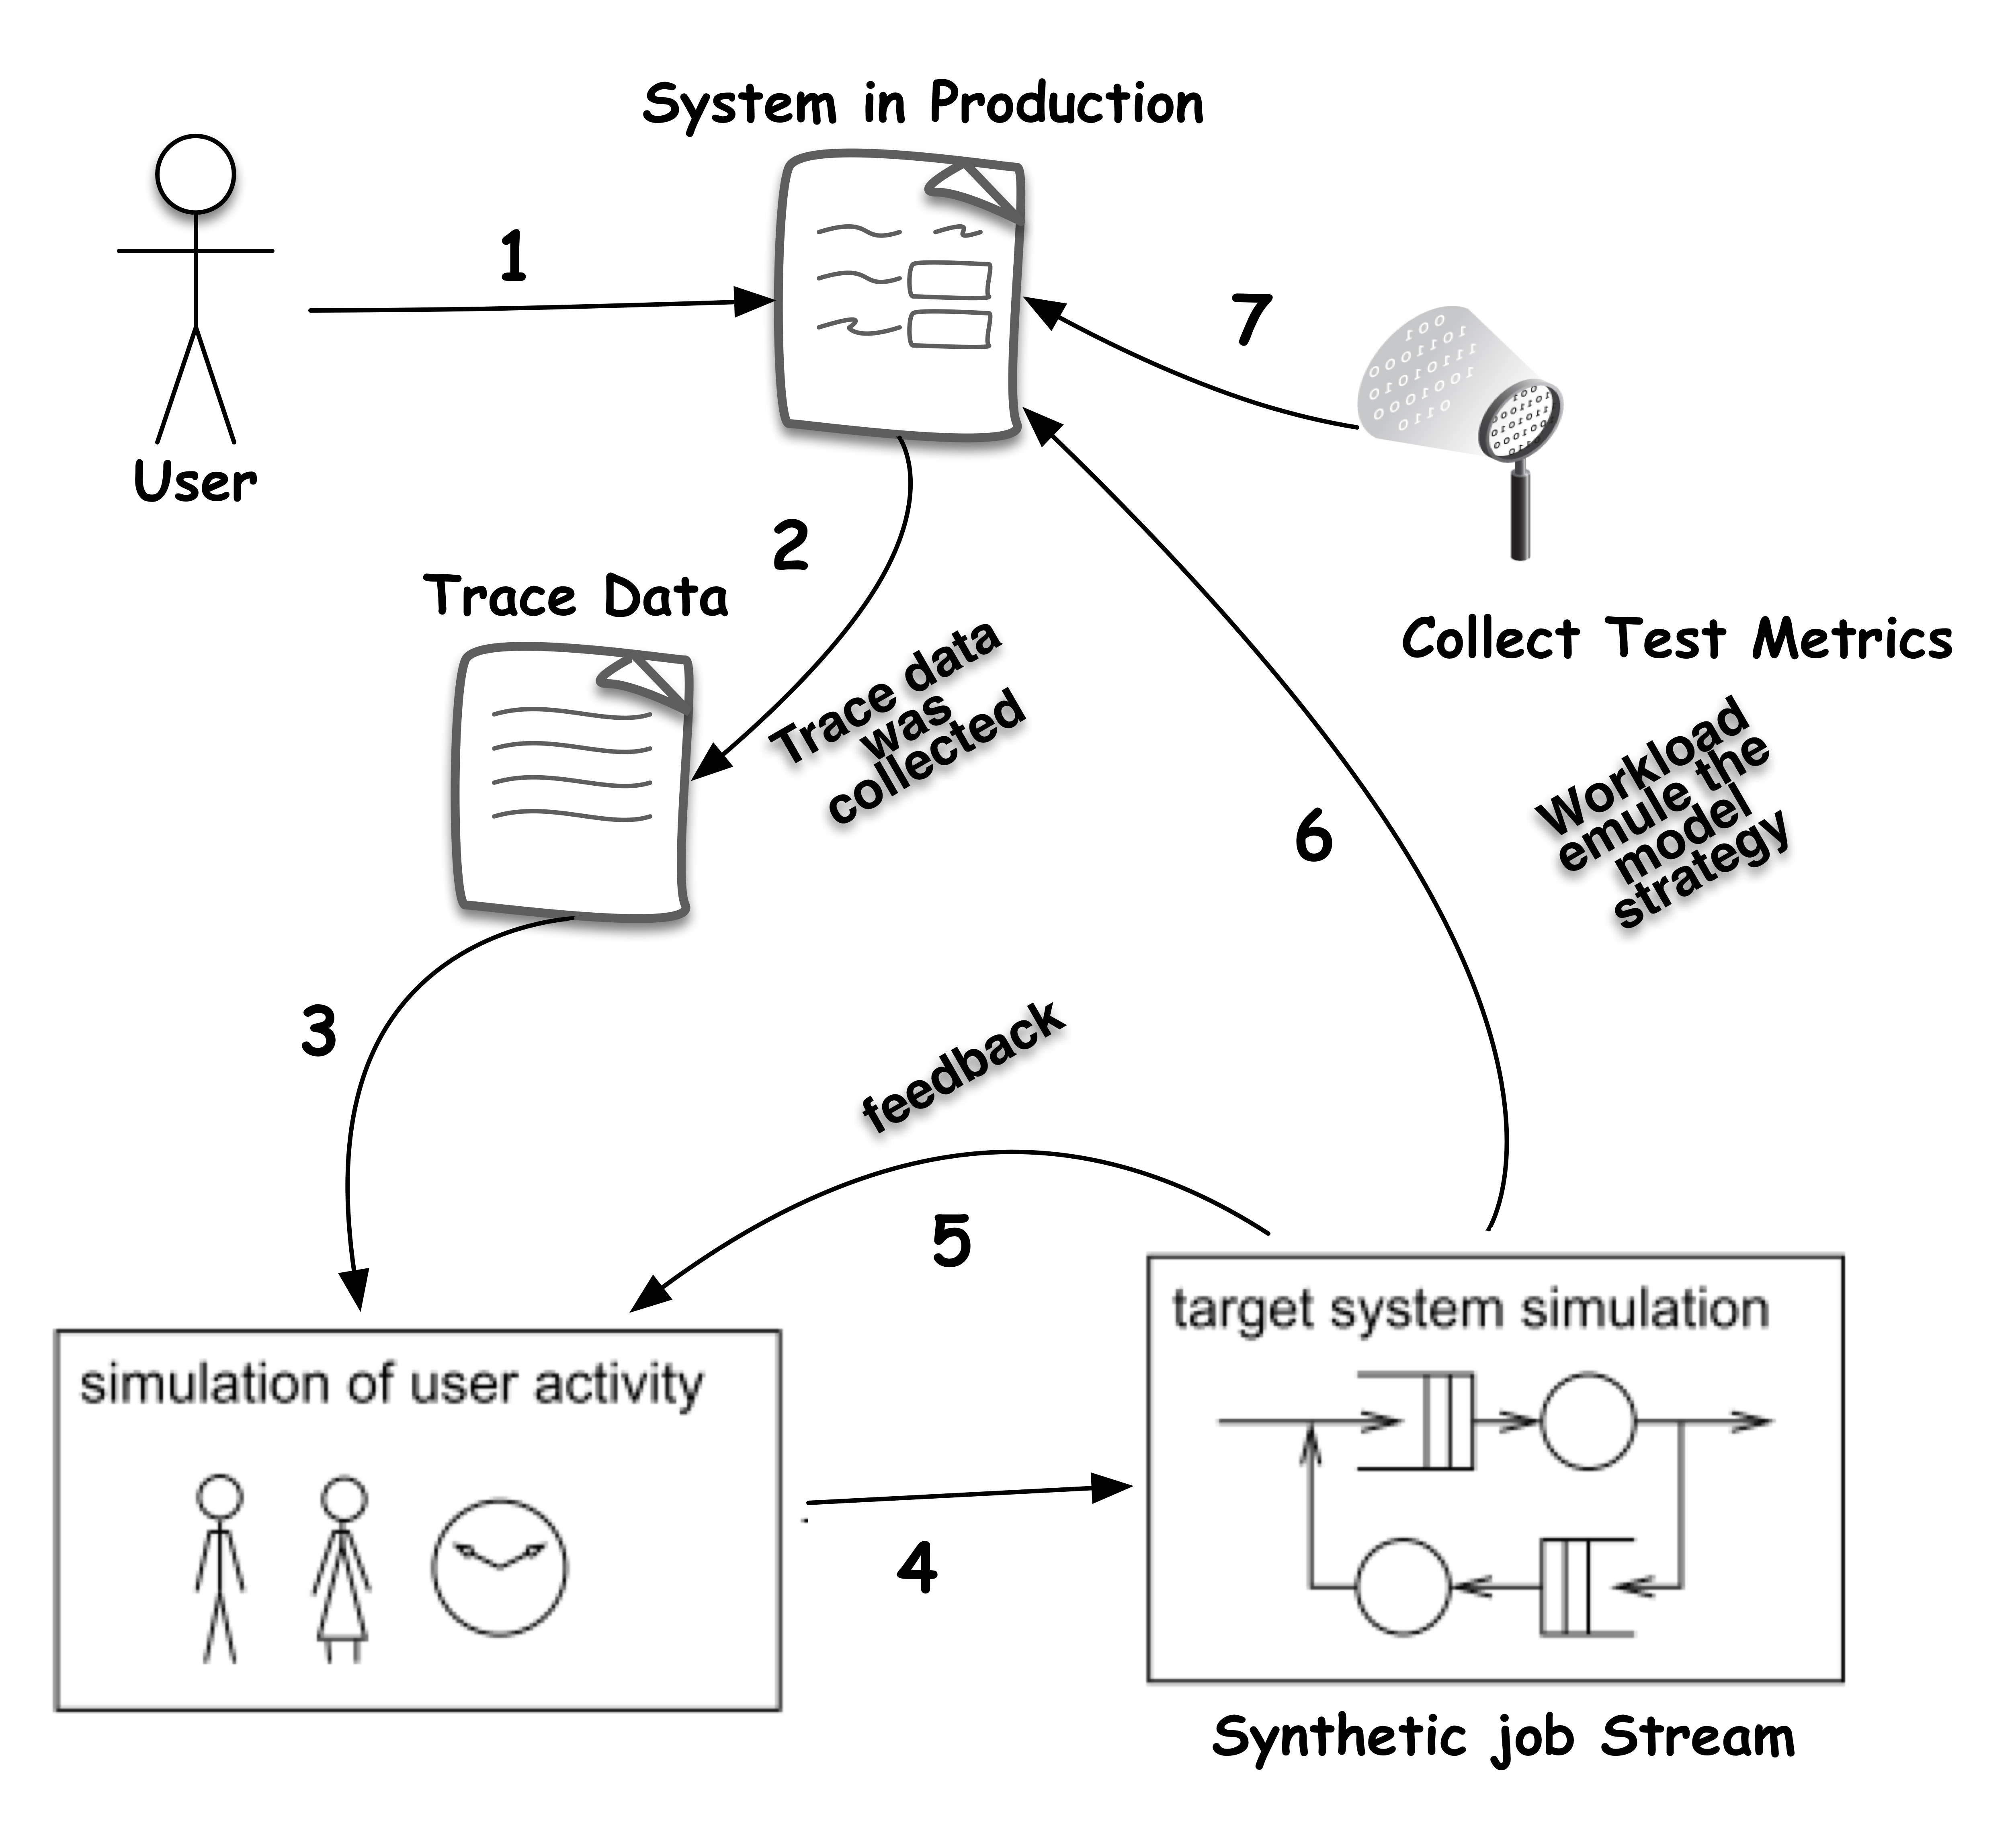
\includegraphics[width=0.6\textwidth]{./images/workloadmodel2300dpi.png}
\caption{Workload modeling based on the generative model \cite{DiLucca2006}}
\label{fig:generativemodel}

\end{figure}


Both load models have their advantages and disadvantages. In general, loads resulting from realistic-load based design techniques (Descriptive models) can be used to detect both functional and non-functional problems. However, the test duration is usually longer and the test analysis is more difficult. Loads resulting from fault-inducing load design techniques (Generative models) take less time to uncover potential functional and non-functional problems, where the resulting loads usually only cover a small portion of the testing objectives \cite{Jiang2010}. The presented research work uses a generative model.


There are two main approaches to design generative or descriptive workloads:

\begin{itemize}
\item Model-based Stress testing: a usage model is proposed to simulate users’ behaviors.
\item Search-based Stress testing.
\end{itemize}


A model-based test is an approach that automates test case generation and execution in order to reduce software testing cost. Search-based techniques are commonly used to generate optimal test data that satisfies every transition and constraint in the state model \cite{Saeed2017}. 

Search-Based Stress testing will be detailed explained in chapter 3. Three other approaches use neither a model-based test nor a search-based test.

\subsection{Model-based Stress Testing}

Model-based testing is an application of models to represent the desired behavior of a System Under Test or to represent testing strategies in a test. Some research approaches propose models to simulate or generate realistic loads. Model-based testing (MBT) is a variant of testing that relies on explicit behavior models that encode the intended behaviors of a system under test. Test cases are generated from one of these models or their combination \cite{MarkUtting2012} \cite{Bertolino2008}. There are many different modeling notations that have been used for modeling the behavior of systems for test generation purposes \cite{MarkUtting2012} \cite{Hierons2009}.

\begin{itemize}
\item State-Based (or Pre/Post) Notations. These model a system as a collection of variables, which represent a snapshot of the internal state of the system, plus some operations that modify those variables. Each operation is usually defined by a pre-condition and a post-condition, or the post-condition may be written as explicit code that updates the state \cite{MarkUtting2012}.
\item Transition-based Notations. These focus on describing the transitions between different states
of the system. Typically, they are graphical node-and-arc notations, like finite state machines
(FSMs). Examples of transition-based notations used for MBT include FSMs themselves, state-charts, labeled transition systems and I/O automata \cite{MarkUtting2012}.
\item History-based Notations. These notations model a system by describing the allowable traces
of its behavior over time. Message-sequence charts and related formalism are also included in this group. These are
graphical and textual notations for specifying sequences of interactions between components \cite{MarkUtting2012}.
\item Functional Notations. These describe a system as a collection of mathematical functions. The
functions may be first-order only, as in the case of algebraic specifications, or higher-order, as in
notations like HOL \cite{MarkUtting2012}. Functional models also show the functionality of the system from the user’s perspective \cite{Ye2007}. This research also classified in the functional notation paradigm the studies that used more than one UML diagram. 
\item Operational Notations. These describe a system as a collection of executable processes,
executing in parallel. They are particularly suited to describing distributed systems and
communications protocols. Examples include process algebras such as CSP or CCS as well as
Petri net notations. Slightly stretching this category, hardware description languages like VHDL
or Verilog are also included in this category \cite{MarkUtting2012}.
\item Stochastic Notations. These describe a system by a probabilistic model of the events and input
values and tend to be used to model environments rather than SUTs. For example, Markov chains
are used to model expected usage profiles, so that the generated tests scenarios \cite{MarkUtting2012}.
\item Data-Flow Notations. These notations concentrate on the data rather than the control flow.
Prominent examples are Lustre, and the block diagrams of Matlab Simulink, which are often used
to model continuous systems \cite{MarkUtting2012}.
\end{itemize}


Table \ref{modelsummary} presents the papers found by the survey about model-based tests. All results were classified by model and paradigm. The most used paradigms in model-based stress testing are  Functional-based notations, Stochastic notations, Transition-based and State-based notations. 

% Please add the following required packages to your document preamble:
% \usepackage{multirow}
% \usepackage[table,xcdraw]{xcolor}
% If you use beamer only pass "xcolor=table" option, i.e. \documentclass[xcolor=table]{beamer}
\begin{table}[h]
\centering
\caption{Summary of studies in model-based stress testing}
\label{modelsummary}
\begin{tabular}{|l|l|l|l|}
\hline
\rowcolor[HTML]{C0C0C0}
\textbf{Model}                          & \textbf{Paper}          & \textbf{Paradigm}    & \textbf{Year} \\ \hline
BeliefDesire-Intention                  & \cite{Araiza-Illan2016} & Operational          & 2016          \\ \hline
                                        & \cite{Avritzer1995b}    & Stochastic Notation         & 1995          \\ \cline{2-4}
                                        & \cite{Barros2007}       & Stochastic Notation        & 2007          \\ \cline{2-4}
                                        & \cite{Avritzer1994}     & Stochastic Notation        & 1994          \\ \cline{2-4}
\multirow{-4}{*}{Markov-Chains}         & \cite{Avritzer1993}     & Stochastic Notation         & 1993          \\ \hline
MCM Model                               & \begin{minipage}{0.4\textwidth}\cite{Wieczorek2010}\end{minipage}    & State-based          & 2010          \\ \hline
                                        & \begin{minipage}{0.4\textwidth}\cite{Enoiu2013}\end{minipage}        & UPPAAL model checker & 2013          \\ \cline{2-4}
\multirow{-2}{*}{Other Approaches}       & \begin{minipage}{0.4\textwidth}\cite{Arcaini2015}\end{minipage}      & Model Decomposition  & 2015          \\ \hline
Petri Nets                              & \cite{Buchs2009}        & Operational          & 2009          \\ \hline
                                        & \cite{Cai2007}          & Stochastic Notation    & 2007          \\ \cline{2-4}
                                        
                                        
                                                                                & \cite{Menasce2002a}          & Stochastic Notation    & 2002          \\ \cline{2-4}
\multirow{-3}{*}{Stochastic Form Model} & \cite{Draheim2006b}     & Stochastic Notation     & 2006          \\ \hline
                                        & \cite{Fang2012}         & State-based          & 2012          \\ \cline{2-4}
                                        & \begin{minipage}{0.4\textwidth} \cite{Sridhar2013} \end{minipage}      & State-based          & 2013          \\ \cline{2-4}
                                        & \cite{Ganesan2016}      & Transition-based     & 2016          \\ \cline{2-4}
                                        & \cite{SanMiguel2016}    & -                    & 2016          \\ \cline{2-4}
                                        & \cite{Arantes2014}      & Transition-based     & 2014          \\ \cline{2-4}
                                        & \begin{minipage}{0.4\textwidth} \cite{Gay2016} \end{minipage}          & Transition-based     & 2016          \\ \cline{2-4}
                                        & \cite{Hessel2007}       & Transition-based     & 2007          \\ \cline{2-4}
                                        & \cite{Hierons2009}      & Transition-based     & 2009          \\ \cline{2-4}
\multirow{-9}{*}{State-Machine Models}  & \cite{Jeong2016}        & State-based          & 2016          \\ \hline
\begin{minipage} {.2\textwidth}
An orchestrated survey of methodologies for automated software test case generation \end{minipage}                           & \cite{Anand2013}        &   ---     & 2013          \\ \hline
\begin{minipage} {.2\textwidth}
Survey on Model-based Testing of Web Applications \end{minipage}                         &
\cite{Wang2013}    & ---          & 2013          \\ \hline
UCML                                        & \cite{Barber1999}       & Functional     & 1999          \\ \hline                                         & \cite{XinyingCai2007}   & Functional           & 2007          \\ \cline{2-4}
                              
                                        & \cite{Rauf2009}         & Functional           & 2009          \\ \cline{2-4}
                                        & \cite{Schaefer2013}     & Functional           & 2013          \\ \cline{2-4}
                                        & \cite{Paper2014}        & Functional           & 2014          \\ \cline{2-4}
                                        & 
\cite{moscher2017facing}        & Functional           & 2017          \\ \cline{2-4}
                                        & \cite{Kim2005}          & Functional           & 2005          \\ \cline{2-4}
                                        & \cite{Rodrigues2014}    & Functional           & 2014          \\ \cline{2-4}
                                        & \begin{minipage}{0.4\textwidth}\cite{Silveira2011}\end{minipage}     & Functional           & 2011          \\ \cline{2-4}
                                        &
\cite{Vogele2016}    & Transition-based      & 2016          \\ \cline{2-4}
&
\cite{DiAlesio2017}   & Functional      & 2017          \\ \cline{2-4}


\multirow{-10}{*}{UML}                   & \begin{minipage}{0.4\textwidth}\cite{Lenz2007}\end{minipage}         & Transition-based           & 2007          \\ \hline
\end{tabular}
\end{table}


\subsubsection{Functional Notation}

All possible answers of the system, including exceptions, are defined in the functional
model.  The functional notation defines the authorized input values and models all the possible functional errors during execution \cite{utting2010practical}. Among the several functional model's approaches, we can highlight the User Community Modeling Language (UCML). A UCML is a set of symbols that can be used to create visual system usage models and depict associated parameters \cite{Wang2013}. The Fig. \ref{fig:ucml} shows a sample where all users realize a login into the application under test. Once logged in, 40\% of the users navigate to the application, 30\%  of the users realize downloads. 20\% of users realize uploads and 10\% of users perform deletions. 

Garousi et al. propose derive Stress Test Requirements from a UML model. The input model consists of a number of UML diagrams. Some of them are standard in mainstream development methodologies and others are needed to describe the distributed architecture of the system under test (Fig. \ref{fig:modelbased}). Cai and Zeng use activity diagrams to describe variation points in use cases. Variation points describe what varies between the applications of a software product line \cite{XinyingCai2007}. Raulf et al. present an approach for testing of web service compositions using UML profile for Business Process Execution Language (BPEL) \cite{Rauf2009}. Schaefer et al. present the Crushinator, a framework that provides a game-independent testing tool simulating clients that perform HTTP requests using a UML model \cite{Schaefer2013}. Moscher and  Fögen compare the techniques Capture and Replay (CR) and Model-Based Testing (MBT) are using a model named PLeTsPerf. PLeTsPerf describes the system under tests using use cases and activity diagrams \cite{moscher2017facing}. Kim proposes an approach to generate massive virtual clients and realistic traffic. A session is composed of a series of the expected operations made by a user in the target domain using a UML class and a sequence diagram \cite{Kim2005}.



\subsubsection{Stochastic Notation}


For many software programs, probabilistic models are a useful asset in
modeling statistical behavior, such that coverage testing is possible by automating
test-case selection, execution and evaluation. Usually, the stochastic notations are used in Markov Chains and Stochastic Formcharts. 

Avritzer and Weyuker present two variants Markov chain approach to realize load and stress tests and an automatic generation of load test suites approach \cite{Avritzer1993} \cite{Avritzer1995b}. Barros et al. provide techniques for load pattern characterization via the application of Markov Chains to performance evaluation of stateful systems \cite{Barros2007}. Cai et al. use a stochastic form chart as its client loading model \cite{Cai2007}. The work of Draheim and Weber’s Form-oriented analysis is a methodology for the specification of ultra-thin client based systems. Form-oriented models describe a web application as a bipartite state machine which consists of pages, actions, and transitions between them. Stochastic Formcharts are the combination of form-oriented model and probability features. The Fig. \ref{fig:stform} shows a sample where all users have a probability of 100\% of realizing a login into the application under test. Once logged in, users have a probability of 40\% of navigating on the application and so on \cite{Draheim2006b} \cite{Marinescu2015}.


\begin{figure}[!ht]
\begin{minipage}{1\textwidth}
\centering
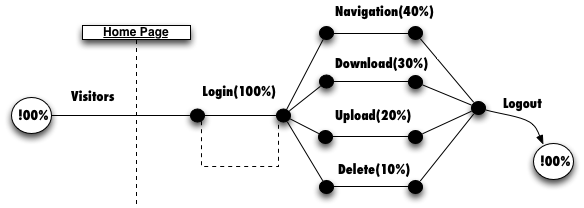
\includegraphics[width=0.6\textwidth]{./images/ucml.png}
\caption{User community modeling language \cite{Wang2013}}
\label{fig:ucml}
\end{minipage}
\begin{minipage}{1\textwidth}
\begin{minipage}{.5\textwidth}
\centering
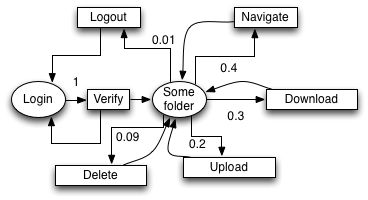
\includegraphics[width=1\textwidth]{./images/stochastic.png}
\caption{Stochastic Formcharts Example \cite{Draheim2006b} \cite{Wang2013}}
\label{fig:stform}
\end{minipage}
\begin{minipage}{.5\textwidth}
\centering
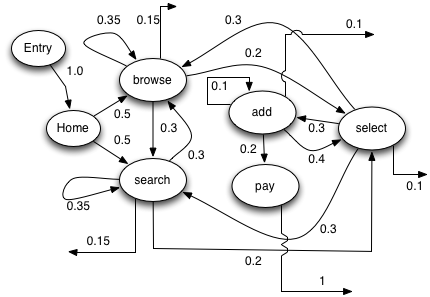
\includegraphics[width=1\textwidth]{./images/cbmg.png}
\caption{Example of a Customer Behavior Model Graph (CBMG)  \cite{Menasce2002a} \cite{Jiang2010} \cite{MohammadS.Obaidat}}
\label{fig:cbmg}
\end{minipage}
\end{minipage}
\end{figure}

One way to capture the navigational pattern within a session is through the Customer Behavior Model Graph (CBMG). Figure \ref{fig:cbmg} depicts an example of a CBMG showing that customers may be in several different states—Home, Browse, Search, Select, Add, and Pay—and they may transition between these states as indicated by the arcs connecting them. The numbers on the arcs represent transition probabilities. A state not explicitly represented in the figure is the Exit state \cite{Menasce2002a} \cite{Jiang2010} \cite{MohammadS.Obaidat}.



\subsubsection{Transition-based notation}


For model-based testing, the transition-based notations are the most used for developing behavioral models \cite{utting2010practical}. Broadly speaking, the
transition-based notations are best for control-oriented applications. Instead of characterizing the system based on its admissible states, the system is characterized as transitions from one state to another, the properties are specified as a set of transitions functions, which
map each input state to the corresponding output state. Based on the notations
used, the model can be annotated with triggering events, which are
conditions sufficient for the transition to take place, or guards that are necessary
preconditions for the transition to be fired. The common techniques used for generating test-cases from transition-based notations are Finite State Machines (FSM), Labeled Transition Systems and UML state-charts \cite{Marinescu2015}.

Arantes et al. present a tool named WEB-PerformCharts that generate test cases using state-charts or FSMs \cite{Arantes2014}. Gay et al. present propose an automated steering framework that can adjust the behavior of the model to better match the behavior of the system under test to reduce the rate of false positives.  The model describes as a transition system \cite{Gay2016}. Hessel addressed in her study two model-based problems: how to formalize coverage criteria and how to generate a test suite to a formal timed system model \cite{Hessel2007}. Ganesan describes how we created a test automation architecture for testing concurrent inter-task communication as carried out by the software bus. The model uses an FSM \cite{Ganesan2016}. Hierons et al. show a formal specification approach to support functional or non-functional tests \cite{Hierons2009}. Vogele et al. present an approach that aims to automate the extraction and transformation of workload specifications for a model-based performance prediction of session-based application systems.  The research also presents transformations to the common load testing tool Apache JMeter and to the Palladio Component Model \cite{Vogele2016} \cite{utting2010practical}. The workload specification formalism (Workload Model) consists of the following components, which are detailed below and illustrated in Fig. \ref{fig:vogel}:
\begin{itemize}
\item An Application Model, specifying allowed sequences of service invocations and SUT-specific details for generating valid requests.
\item A set of Behavior Models, each providing a probabilistic representation of user sessions in terms of invoked services.
\item A Behavior Mix, specified as probabilities for the individual Behavior Models to occur during workload generation.
\item A Workload Intensity that includes a function which specifies the number of concurrent users during the workload generation execution.
\end{itemize}

\begin{figure}[!ht]
\begin{minipage}{.5\textwidth}
\centering
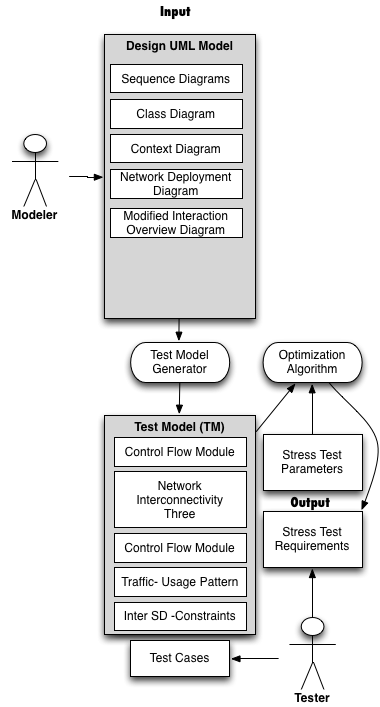
\includegraphics[width=1\textwidth]{./images/modelmethodology.png}
\caption{Model-based stress test methodology}
\label{fig:modelbased}
\end{minipage}
\begin{minipage}{.5\textwidth}
\centering
\centering
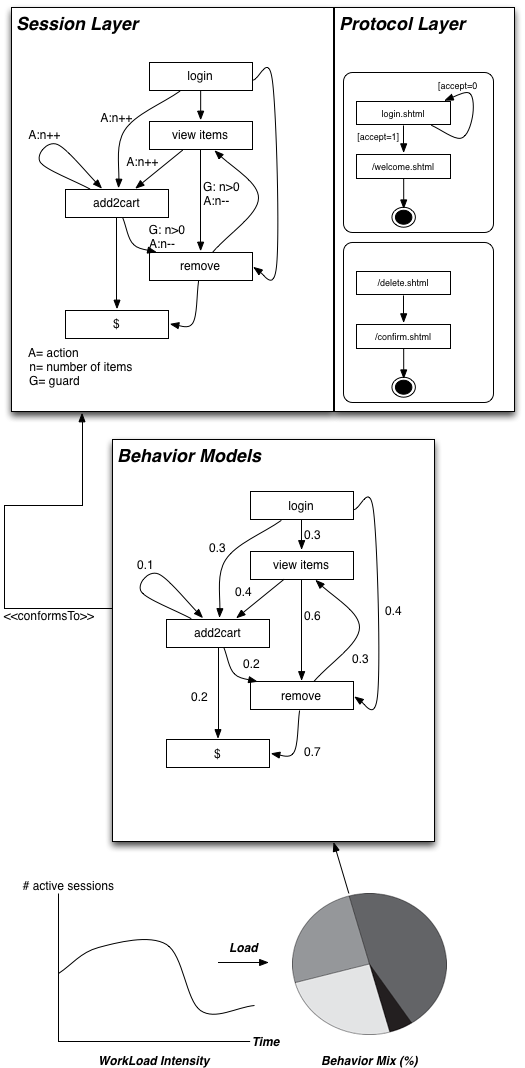
\includegraphics[width=1\textwidth]{./images/vogel.png}
\caption{Exemplary workload model}
\label{fig:vogel}


\end{minipage}
\end{figure}

\begin{figure}[!ht]
\centering
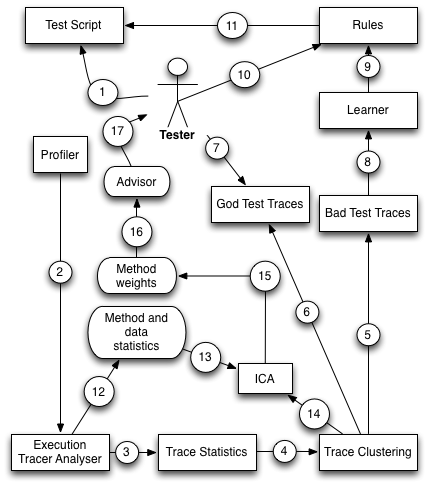
\includegraphics[width=0.6\textwidth]{./images/FOREPOST.png}
\caption{The architecture and workflow of FOREPOST}
\label{fig:forepost}

\end{figure}


\subsubsection{State-based notation}

State based notations like STATECHARTS
or activity diagrams describe the behavior based on abstract
states and support behavior integration only using
state composition \cite{Giese1999}. In State-based or notations, the system is modeled as a collection of variables representing its state at a specific point of the execution, together with a collection of operations defined by a precondition that defines the
admissible set of initial states, and a postcondition that specifies the guaranteed
set of final states. Examples of such notations include the Z language, the
B machine, UML’s Object Constraint Language (OCL), Java Modeling
Language (JML), VDM , and Spec\# \cite{Marinescu2015}.

Sridhar proposed an approach to generate test cases with MATLAB using Simulink/ Stateflow tool. After the model creation, test sequences are generated a dependency graph of that system \cite{Sridhar2013}.  Fang et al. developed a test case generator, from which an entire test suite can be extracted \cite{Fang2012}.  Jeong et al. propose
a state transition model based to test case generation \cite{Jeong2016}. Wieczorek et al. propose an approach that uses proprietary models called Message Choreography Models (MCM) using a state-based representation \cite{Wieczorek2010}.




\subsection{Other Approaches}

A set of other approaches don't use model-based tests or search-based tests:

\begin{itemize}
\item Automatic feedback, control-based, stress and load testing \cite{Bayan2008};
\item Feedback-ORiEnted PerfOrmance Software Testing \cite{Luo2015};
\item PASASM: A Method for the
Performance Assessment of Software Architectures \cite{Williams2002}.
\end{itemize}

Bayan and Cangussu present an approach based on the application of a feedback
PID (Proportional, Integral, and Derivative) controller to drive the input and make the system achieve a specified level of resource usage. For example, if the user defines the system should be tested with a memory use of 95\%, starting from an initial input value, the PID controller will automatically change the input(s) until the desired level of stress has been achieved \cite{Bayan2008}.

Williams and Smith describe the PASA method, a method for performance assessment of software architectures. PASA uses the principles and techniques of software performance engineering (SPE) to determine whether an architecture is capable of supporting its performance objectives  \cite{Williams2002}. Among the three approaches presented, we can highlight FOREPOST that develops a plugin of the JMeter tool to generate test cases using unsupervised learning.

\subsubsection{Feedback-ORiEnted PerfOrmance Software Testing}

Feedback-ORiEnted PerfOrmance Software Testing (FOREPOST) is an adaptive, feedback-directed learning testing system that learns rules from system execution traces and uses these learned rules to select test input data automatically to find more performance problems in applications when compared to exploratory random performance testing \cite{Grechanik2012}.

FOREPOST uses runtime monitoring for a short duration of testing together with machine learning techniques and automated test scripts to reduce large amounts of performance-related information collected during AUT runs to a small number of descriptive rules that provide insights into properties of test input data that lead to increased computational loads of applications.

The Fig. \ref{fig:forepost} presents the main workflow of FOREPOST solution. The first step,  The Test Script is written by the test engineer(1). Once the test script starts, its execution traces are collected (2) by the Profiler, and these traces are forwarded to the Execution Trace Analyzer, which produces (3) the Trace Statistics. The trace statistics is supplied (4) to Trace Clustering, which uses an ML algorithm, JRip to perform unsupervised clustering of these traces into two groups that correspond to (6) Good and (5) Bad test traces.

The user can review the results of clustering (7). These clustered traces are supplied (8) to the Learner that uses them to learn the classification model and (9) output rules. The user can review (10) these rules and mark some of them as erroneous if the user has sufficient evidence to do so. Then the rules are supplied (11) to the Test Script. Finally, the input space is partitioned into clusters that lead to good and bad test cases, to find methods that are specific to good performance test cases. This task is accomplished in parallel to computing rules, and it starts when the Trace Analyzer produces (12) the method and data statistics that are used to construct (13) two matrices (14). Once these matrices are constructed, ICA\footnote{ICA is a technique to separate linearly mixed sources \cite{Luo2015}} decomposes them (15) into the matrices for bad and good test cases correspondingly. Finally, the Advisor (16) determines top methods that performance testers should look at (17) to debug possible performance problems.

\section{Research Question 2: What are the main anti-patterns found by stress tests?}

 Performance problems share common symptoms and many performance problems described in the literature are defined by a particular set of root causes. Fig. \ref{fig:symptoms}  shows the symptoms of known performance problems \cite{Wert2013a}.



\begin{figure}[h]
\centering
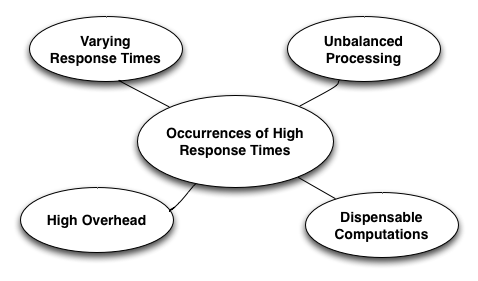
\includegraphics[width=0.6\textwidth]{./images/Symptoms.png}
\caption{Symptoms of known performance problems \cite{Wert2013a}. }
\label{fig:symptoms}
\end{figure}


There are several anti-patterns that detailed features about  common performance problems. Antipatterns are conceptually similar to patterns in that they document recurring solutions to common design problems. They are known as
antipatterns because their use produces negative consequences.

% Please add the following required packages to your document preamble:
% \usepackage{multirow}
% \usepackage[table,xcdraw]{xcolor}
% If you use beamer only pass "xcolor=table" option, i.e. \documentclass[xcolor=table]{beamer}
\begin{table}[!h]
\centering
\caption{Performance anti-patterns}
\label{antipatterns}
\begin{tabular}{|l|l|l|llll}
\cline{1-3}
\multicolumn{2}{|l|}{\cellcolor[HTML]{C0C0C0}\textbf{Antipattern}}     & \cellcolor[HTML]{C0C0C0}\textbf{Papers}                                                                        &  &  &  &  \\ \cline{1-3}
Blob or The God Class                   &                              & \begin{minipage}{0.3\textwidth} \cite{Wert2014} \\ \cite{Smith2000} \\ \cite{Trubiani2011} \\\cite{Vetoio2011} \\ \cite{Cortellessa2007} \\\cite{Smith2003} \end{minipage} &  &  &  &  \\ \cline{1-1} \cline{3-3}
Circuitous Treasure Hunt                &                              & \begin{minipage}{0.4\textwidth} \cite{Wert2014} \\ \cite{Trubiani2011}  \\ \cite{Vetoio2011} \\ \cite{Smith2003} \\ \cite{Smith2002} \end{minipage}                        &  &  &  &  \\ \cline{1-1} \cline{3-3}
Empty Semi Trucks                       &                              & \begin{minipage}{0.3\textwidth} \cite{Wert2014} \\\cite{Trubiani2011} \\ \cite{Arcelli2012} \\ \cite{Vetoio2011}                                       \end{minipage} &  &  &  &  \\ \cline{1-1} \cline{3-3}
\begin{minipage}{0.3\textwidth} Excessive Dynamic\\ Allocation  \end{minipage}          &                              & \begin{minipage}{0.4\textwidth} \cite{Trubiani2011} \\ \cite{Vetoio2011} \\ \cite{Smith2003} \\ \cite{Smith2002} \end{minipage}                                       &  &  &  &  \\ \cline{1-1} \cline{3-3}
More is Less                            &                              &  \begin{minipage}{0.4\textwidth} \cite{Vetoio2011} \\\cite{Trubiani2011} \\ \cite{Smith2003}   \end{minipage}                                                        &  &  &  &  \\ \cline{1-1} \cline{3-3}
One-Lane Bridge                         &                              &  \begin{minipage}{0.4\textwidth} \cite{Vetoio2011} \\ \cite{Trubiani2011} \\ \cite{Smith2003} \\ \cite{Smith2002}                                        
  
  \end{minipage}
&  &  &  &  \\ \cline{1-1} \cline{3-3}
Stifle                                  &                              & \cite{Wert2014}                                                                                                &  &  &  &  \\ \cline{1-1} \cline{3-3}
The Ramp                                &                              & \begin{minipage}{0.4\textwidth}\cite{Trubiani2011} \\ \cite{Vetoio2011} \\ \cite{Smith2003}   \end{minipage}                                                        &  &  &  &  \\ \cline{1-1} \cline{3-3}
Tower of Babel                          &                              & \begin{minipage}{0.4\textwidth}\cite{Trubiani2011} \cite{Vetoio2011}   \end{minipage}                                                                        &  &  &  &  \\ \cline{1-1} \cline{3-3}
Traffic Jam                             & \multirow{-10}{*}{}          & \begin{minipage}{0.4\textwidth}\cite{Vetoio2011} \\ \cite{Smith2003} \\ \cite{Smith2002} \end{minipage}                                                            &  &  &  &  \\ \cline{1-3}
                                        &                              &\begin{minipage}{0.4\textwidth} \cite{Cortellessa2007} \cite{Trubiani2011} \cite{Smith2003} \end{minipage}                                                     &  &  &  &  \\ \cline{2-3}
                                        & Concurrent Processing System & \begin{minipage}{0.4\textwidth} \cite{Vetoio2011} \cite{Smith2003} \end{minipage}                                                                             &  &  &  &  \\ \cline{2-3}
                                        & Piper and Filter             & \begin{minipage}{0.4\textwidth} \cite{Vetoio2011} \\ \cite{Smith2003}  \end{minipage}                                                                            &  &  &  &  \\ \cline{2-3}
\multirow{-4}{*}{Unbalanced Processing} & Extensive Process            & \begin{minipage}{0.4\textwidth} \cite{Vetoio2011} \cite{Smith2003}   \end{minipage}                                                                           &  &  &  &  \\ \cline{1-3}
Unnecessary Processing                  &                              & \cite{Smith2003}                                                                                               &  &  &  &  \\ \cline{1-3}
\end{tabular}
\end{table}




Performance anti-patterns document common performance mistakes made in software architectures or designs. These software Performance anti-patterns have four primary uses: identifying problems,
focusing on the
right level of abstraction,
effectively communicating
their causes to others and prescribing solutions \cite{brown1998antipatterns}. Table \ref{antipatterns} present some of the most common performance anti-patterns.


% Please add the following required packages to your document preamble:
% \usepackage{multirow}
% \usepackage[table,xcdraw]{xcolor}
% If you use beamer only pass "xcolor=table" option, i.e. \documentclass[xcolor=table]{beamer}
%\begin{table}[h]
%\centering
%\caption{Performance antipatterns}
%\label{antipatterns}
%\begin{tabular}{|l|l|}
%\hline
%\rowcolor[HTML]{C0C0C0}
%\multicolumn{1}{|c|}{\cellcolor[HTML]{C0C0C0}\textbf{antipattern}} & \multicolumn{1}{c|}{\cellcolor[HTML]{C0C0C0}\textbf{Derivations}} \\ \hline
%Blob or The God Class &  \\ \hline
% & Concurrent processing Systems \\ \cline{2-2}
% & Piper and Filter Architectures \\ \cline{2-2}
%\multirow{-3}{*}{Unbalanced-Processing} & Extensive Processing \\ \hline
%Circuitous Treasure Hunt &  \\ \cline{1-1}
%Empty Semi Trucks &  \\ \cline{1-1}
%Tower of Babel &  \\ \cline{1-1}
%One-Lane Bridge &  \\ \cline{1-1}
%Excessive Dynamic Allocation &  \\ \cline{1-1}
%Traffic Jam &  \\ \cline{1-1}
%The Ramp  &  \\ \cline{1-1}
%More is Less & \multirow{-10}{*}{} \\ \hline
%\end{tabular}
%\end{table}

Blob anti-pattern is known by various names, including the “god” class [8] and the “blob” [2]. Blob is an anti-pattern whose problem is on the excessive message traffic generated by a single class or component, a particular resource does the majority of the work in a software. The Blob occurs when a single class or component either performs all of the work of an application or holds all of the application’s data. Either manifestation results in excessive message traffic that can degrade performance \cite{Cortellessa2007} \cite{Smith2000}.

A project containing a “god” class usually has a single, complex controller class that is surrounded by simple classes that serve only as data containers. These classes typically contain only accessor operations (operations to get() and set() the data) and perform little or no computation of their own \cite{Smith2000}. According to Figure \ref{fig:godclass} and \ref{fig:godclass2}, a hypothetical system with a BLOB problem is shown: Figure \ref{fig:godclass} presents a sample where the Blob class uses the features A,B,C,D,E,F and G of the hypothetical system, and Fig. \ref{fig:godclass2} shows a static view where a complex software entity instance, i.e. Sd, is connected to other software instances, e.g. Sa, Sb and Sc, through many dependencies \cite{Vetoio2011}\cite{Wert2013a}.




\begin{figure}[h]
\begin{minipage}{.5\textwidth}
\centering
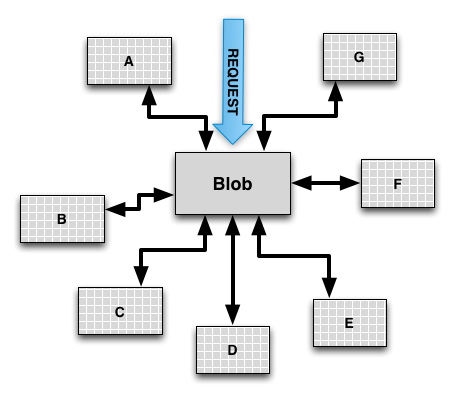
\includegraphics[width=1\textwidth]{./images/BLOB.png}
\captionof{figure}{The God class\cite{Wert2013a}. }
\label{fig:godclass}
\end{minipage}
\begin{minipage}{.5\textwidth}
\centering
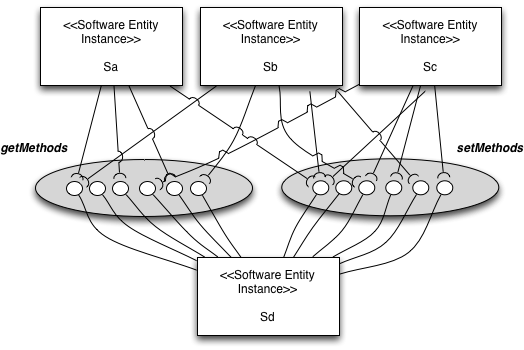
\includegraphics[width=1\textwidth]{./images/blob2.png}
\captionof{figure}{The God class\cite{Vetoio2011}. }
\label{fig:godclass2}
\end{minipage}
\end{figure}

A characteristic of Unbalanced Processing is the tendency to overload a particular resource, wherein one scenario a specific class of requests generates a pattern of execution within the system. In other words, the overloaded resource will be executing a certain type of job very often, thus in practice damaging other classes
of jobs that will experience very long waiting times. Unbalanced Processing occurs in three different situations. The first case that causes unbalanced processing is when processes cannot make effective use of available processors either because processors are dedicated to other tasks or because of single-threaded code. This manifestation has available processors and we need to ensure that the software is able to use them. Fig. \ref{fig:unbalanced}  shows a sample of the Unbalanced Processing. In Fig. \ref{fig:unbalanced}, four tasks are performed. Task D is waiting for task C to conclude, and both are submitted to a heavy processing situation.

\begin{figure}[h]
\centering
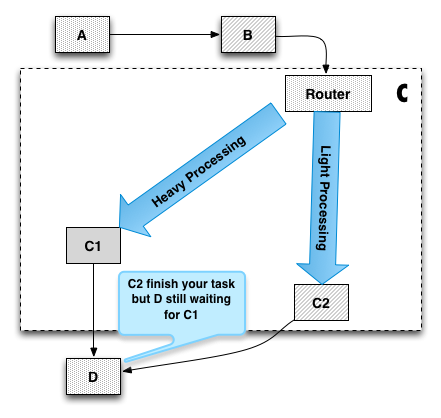
\includegraphics[width=0.7\textwidth]{./images/unbalanced.png}
\caption{Unbalanced Processing sample \cite{Wert2013a}. }
\label{fig:unbalanced}
\end{figure}

The pipe and filter architectures  and extensive processing anti-pattern represent a manifestation of the unbalanced processing anti-pattern. The pipe and filter architectures occur when the throughput of the overall system is determined by the slowest filter. Fig \ref{fig:pipefilter} illustrates a software S with a Pipe and Filter Architectures problem:  the operation opx is invoked in a service  and the throughput of the service (\$Th(S)) is lower than the required one. The extensive processing occurs when a process monopolizes a processor and prevents a set of other jobs to be executed until it finishes its computation. The Fig. \ref{fig:extpro} describes a software S with an Extensive Processing problem: the operations opx and opy are alternatively invoked in a service and the response time of the service (\$RT(S)) is larger than the required one \cite{Vetoio2011}.

\begin{figure}[h]
\begin{minipage}{.5\textwidth}
\centering
\includegraphics[width=1\textwidth]{./images/pipe2.png}
\caption{Pipe and Filter sample \cite{Vetoio2011}}
\label{fig:pipefilter}
\end{minipage}
\begin{minipage}{.5\textwidth}
\centering
\includegraphics[width=1\textwidth]{./images/extpro.png}
\caption{Extensive Processing sample \cite{Vetoio2011}.}
\label{fig:extpro}
\end{minipage}
\end{figure}


Circuitous Treasure Hunt anti-pattern occurs when software retrieves data from a first component, uses those results in a second component, retrieves data from the second component, and so on until the last results are obtained \cite{Smith2002} \cite{Smith2003}. Circuitous Treasure Hunt
are typical performance anti-patterns that cause  unnecessarily high amount of frequent database requests. The Circuitous Treasure Hunt anti-pattern is a result of a bad database schema or query design. A common Circuitous Treasure Hunt design creates a data dependency between single queries. For instance, a query requires the
result of a previous query as input. The longer the chain of
dependencies between individual queries the more the Circuitous
Treasure Hunt hurts performance \cite{Wert2014}. Fig. \ref{fig:circuit}  shows a software S with a Circuitous Treasure Hunt problem: the software  S generates a large number of database calls by performing several queries up to the final operation \cite{Vetoio2011}.


\begin{figure}[h]
\begin{minipage}{.5\textwidth}
\centering
\includegraphics[width=1\textwidth]{./images/circuit.png}
\caption{Circuitous
Treasure Hunt sample \cite{Vetoio2011}}
\label{fig:circuit}
\end{minipage}
\begin{minipage}{.5\textwidth}
\centering
\includegraphics[width=1.2\textwidth]{./images/trucks2.png}
\caption{Empty Semi Trucks sample \cite{Vetoio2011}.}
\label{fig:trucks}
\end{minipage}
\end{figure}

Empty Semi Trucks occurs when an excessive number of requests is required to perform a task. It may be due to inefficient use of available bandwidth, an inefficient interface, or both \cite{Arcelli2012}. There is a special case of Empty Semi Trucks that occurs  when many fields in a user interface must be retrieved from a
remote system. Fig. \ref{fig:trucks} shows a software S with an Empty Semi Trucks problem: the software instance Sa generates an excessive message traffic by sending a high amount of messages with low sizes, much lower than the network bandwidth, hence the network link might have a low utilization value \cite{Vetoio2011}.

The Tower of Babel anti-pattern most often occurs when information is translated into an exchange format, such as XML, where the sending process is then parsed and translated into an
internal format by the receiving process. When the translation and parsing are excessive, the system spends most
of its time doing this and relatively little real work \cite{Smith2003}. Fig. \ref{fig:babel} shows a system with a Tower of Babel problem: the software instances Sd performs the format translation to communicate with other instances many times \cite{Vetoio2011}.

\begin{figure}[H]
\begin{minipage}{.5\textwidth}
\centering
\includegraphics[width=1\textwidth]{./images/babel2.png}
\caption{Tower of Babel sample \cite{Vetoio2011}}
\label{fig:babel}
\end{minipage}
\begin{minipage}{.5\textwidth}
\centering
\includegraphics[width=1\textwidth]{./images/onelane.png}
\caption{One-Lane Bridge sample \cite{Vetoio2011}.}
\label{fig:onelane}
\end{minipage}
\end{figure}


One-Lane Bridge is an anti-pattern that occurs when one or a few processes execute concurrently using a shared resource and while the other processes are waiting to use the shared resource. It frequently occurs in applications that access a database. Here, a lock ensures that only one process may update the associated portion of the database at a time. This anti-pattern is common when many concurrent threads or processes are waiting for the same shared resources. These can either be passive resources (like semaphores or mutexes) or active resources (like CPU or hard disk). In the first case, we have a typical One Lane Bridge whose critical resource needs to be identified. Figure 3.10 shows a system with a One-Lane Bridge problem:  the software instance Sc receives an excessive number of synchronous calls in a service S and the predicted response time is higher than the required one \cite{Vetoio2011}.


Using dynamic allocation, objects are created when they are first accessed and then destroyed when they are no longer needed. Excessive Dynamic Allocation, however, addresses frequent, unnecessary creation and destruction of objects of the same class. Dynamic allocation is expensive, an object created in memory must be allocated from the heap, and any initialization code for the object and the contained objects must be executed. When the object is no longer needed, necessary cleanup must be performed, and the reclaimed memory must be returned to the heap to avoid memory leaks \cite{Smith2002} \cite{Smith2003}.

\begin{figure}[h]
\begin{minipage}{.5\textwidth}
\centering
\includegraphics[width=1\textwidth]{./images/excessivedynamicallocation.png}
\caption{Excessive Dynamic Allocation.}
\label{fig:dynallocation}
\end{minipage}
\begin{minipage}{.5\textwidth}
\centering
\includegraphics[width=1\textwidth]{./images/jam.png}
\caption{Traffic Jam Response Time \cite{Vetoio2011}.}
\label{fig:jam}
\end{minipage}
\end{figure}

Fig. \ref{fig:dynallocation} shows an Excessive Dynamic Allocation sample. This example is drawn from a call (an offHook event) and the switch creates a Call object to manage the call. When the call is completed, the Call object is destroyed. Constructing a single Call object is not as excessive. A Call is a complex object that contains several other objects that must also be created. The Excessive Dynamic Allocation occurs when a switch receives hundreds of thousands of offHook events. In a case like this, the overhead for dynamically allocating call objects adds substantial delays to the time needed to complete a call.

The Traffic Jam anti-pattern occurs if many concurrent threads or processes are waiting for the same  active resources (like CPU or hard disk). This anti-pattern produces a large backlog in jobs waiting for service. The performance impact of the Traffic Jam is the transient behavior that produces wide variability in response time. Sometimes it is fine, but at other times, it is unacceptably long. Figure \ref{fig:jam} exhibits a software with a Traffic Jam problem, in which the monitored response time of the operation shows a wide variability in a response time that persists long \cite{Vetoio2011}.


\begin{figure}[!h]
\begin{minipage}{.5\textwidth}
\centering
\includegraphics[width=0.6\textwidth]{./images/ramp.png}
\caption{The Ramp sample \cite{Vetoio2011}.}
\label{fig:ramp}
\end{minipage}
\begin{minipage}{.5\textwidth}
\centering
\includegraphics[width=1\textwidth]{./images/moreisless.png}
\caption{More is Less sample \cite{Vetoio2011}.}
\label{fig:moreisless}
\end{minipage}
\end{figure}

Ramp is an anti-pattern where the processing time increases as the system is used. Ramp can arise in several different ways. Any situation in which the amount of processing required to satisfy a request increases over time will produce the behavior. With the Ramp anti-pattern, the memory consumption of the application is growing over time. The root causes are the Specific Data Structures, which are growing during operation or which are not properly disposed \cite{Wert2014} \cite{Smith2003}. Fig. \ref{fig:ramp} shows a system  with the Ramp problem:  (i) the monitored response time of the operation opx at time t1, i.e. \$RT(opx, t1), is much lower than at time t2, i.e. \$RT(opx, t2), with t1 < t2; (ii) the monitored throughput of the operation opx at time t1, i.e. \$Th(opx, t1), is much larger than at time t2, i.e. \$Th(opx, t2), with t1 < t2.

More is Less occurs when a system spends more time "thrashing” than accomplishing real work because there are too many processes relative to available resources. More is Less is presented when it is running too many programs over time. This anti-pattern causes too much system paging and systems spend all their time servicing page faults rather than processing requests. In distributed systems, there are more causes. They include: creating too many database connections and  allowing too many internet connections. Fig. \ref{fig:moreisless} illustrates a system  with a More Is Less problem: There is a processing node PN1 and the monitored runtime parameters (e.g. database connections, etc.) at time t1, i.e. \$Par(PN1[p], t1), are much larger than the same parameters at time t2, i.e. \$Par(PN1[p], t2), with t1 < t2.

\section{Summary}

Stress testing investigates the behavior of the system under conditions
that overload its resources \cite{Sandler2004} \cite{Lewis2005}. The core activities in conducting a usual Load, Performance and Stress tests are  Identify the test environment, Identify acceptance criteria, Plan and design tests, Prepare the test environment, Record the test plan, Run the tests and Analyze results. This research focuses on the generation and execution of test cases. It is not the scope of the research the automatic analysis of the results and the treatment of log of tests. The two main approaches to creating workloads are generative and descriptive workload approaches. The main goal of descriptive workloads is to ensure that the system can function correctly once. Generative workloads  aims to design loads, which are likely to cause a functional or non-functional problem. 

There are three approaches to stress test execution: Live-User Based Executions, Driver Based Executions and Emulation Based Executions. This thesis focuses on user Driver Based Executions where each workload performs several requests to an application under test to measure the response time. Apache JMeter was the tool chosen for current research due to its open license, the use of plugins and the ease of integration with jmetal and jgap frameworks.

The main approaches to generate test cases to stress testing are: Model-based testing and Search-based testing. Model-based testing uses a model to describe the states and transitions of a system under test. Although the use of models allows greater control of generated test cases, since all test cases are generated from the previously defined model, it is also the main limitation of this approach since the model may not include all possible scenarios of the test because it depends intrinsically on the test designer responsible for creating the models. The most used paradigms in model-based stress testing are:  Functional-based notations, Stochastic notations, Transition-based and State-based notations. 

There are several anti-patterns that detailed features about common performance problems. Antipatterns
are conceptually similar to patterns in that they document recurring solutions to common design problems. This survey found 10 anti-patterns of which 4 were  implemented by IAdapter in an experiment presented in chapter 4.


\chapter{Adapted SEDR}


Software is pervasive, which raises the value of testing it \cite{Sandler2004}. Various actions outside the application under test can cause high response times such as pagination, network usage or even a software upgrade. It is necessary a noise reduction strategy in stress test in this situations. Noisy optimization is currently receiving increasing popularity for its widespread applications in engineering optimization
problems, where the objective functions are often found to be contaminated with noisy \cite{Rakshit2017}. 


Standard Error Dynamic Resampling (SEDR), the strategy has been employed for solving both noisy single and multi-objective evolutionary
optimization problems. The working principle of SEDR is to add samples to a solution sequentially until the standard error of
the objectives fall below a chosen threshold value \cite{Siegmund2013}. It was proposed in \cite{DiPietro2004} for single-objective optimization problems. In this study, we apply SEDR on multi-objective problems by aggregating all objective values to a scalar value. As aggregation, the median of the objective standard errors is used. The strategy is concerned with the optimal allocation of sampling budget to a trial solution based on the noise strength at its corresponding position in the search space. The contamination level of noise is captured by the standard error of the mean fitness estimate of a trial solution. The SEDR algorithm is described in Alg. \ref{SEDR}.


\begin{algorithm}[h]
  \caption{SEDR algorithm \cite{Siegmund2013}}\label{SEDR}
  \begin{algorithmic}[1]

    \State \textbf{input :} Solution s
    \State Draw $b_{min}\ge 2$ initial samples of s, F(s)
    \State Calculate mean of the available fitness for each of the \textit{m} objectives: $\mu_{i}(s)$, i=1,...,m
    \State Calculate standard deviation: $\sigma_{i}=\sqrt{ \frac{1}{n-1} \sum_{n}^{j=1} (F^i_{j}-\mu_{i}(s))^2} $
    \State Calculate the standard error: $se_{i}(s)=\frac{\sigma_{i}}{\sqrt{n}}$
    \State Calculate an aggregation of the standard errors $\overline{se}(s)$
    \State Stop if  $\overline{se}(s)$ > threshold or $b_{s}\ge b_{max}$ otherwise go to step 2
  \end{algorithmic}
\end{algorithm}



\begin{figure}[!h]
\centering
\includegraphics[width=0.8\textwidth]{./images/outliers.png}
\caption{Results obtained without Noise Reduction}
\label{fig:outliers}
\end{figure}




Numerous tests in this research obtained response times higher than similar scenarios in other executions. After assessing the obtained results, we found that one of the reasons for higher response time is the occurrence of disk pagination. In order to more accurately test the response times of the outliers, we put forward an adaptation of the SEDR algorithm. Fig. \ref{fig:outliers} presents the results without a Noise Reduction algorithm.  

SEDR noise reduction is used by this research in multi-objective scenarios experiments where the objective of the experiments besides finding the tests with the longest response time also needs to find the Pareto frontier of the application. 

\begin{figure}[!h]
\centering
\includegraphics[width=0.8\textwidth]{./images/suspectlist.png}
\caption{SEDR customized algorithm}
\label{fig:sedrcustomized}
\end{figure}


The experiments use a customized version of the SEDR algorithm for noise reduction. The algorithm runs as long as each workload has at least 3 samples or the SEDR condition is satisfied for all workloads ( Figure \ref{fig:sedrcustomized} - \ding{202}). The algorithm adds all workloads in OUTLIERS list to the list of execution ( Figure \ref{fig:sedrcustomized} - \ding{203}). All workloads are performed and the SEDR condition is verified  ( Figure \ref{fig:sedrcustomized} - \ding{204} and \ding{205} ). If the SEDR condition is satisfied the workload is removed from OUTLIERS list ( Figure \ref{fig:sedrcustomized} - \ding{206}) otherwise the workload is included in the list if it is no longer present ( Figure \ref{fig:sedrcustomized} - \ding{207}). 





\chapter{IAdapter }

This Appendix presents the IAdapter tool used by this research and a survey study to assess the use of the tool by the non-functional test team of the Serpro, a company of the Brazilian Federal Government in Fortaleza. 


IAdapter is a JMeter plugin designed to perform search-based stress tests. Fig. \ref{fig:iadapterlifecycle} presents the IAdapter Life Cycle. The main difference between IAdapter and JMeter tool is that the IAdapter provide an automated test execution where the new test scenarios are chosen by the test tool.  In a test with JMeter, the tests scenarios are usually chosen by a test designer.

\begin{figure}[h]
\centering
\includegraphics[width=0.7\textwidth]{./images/lifecycle2.png}
\caption{IAdapter life cycle}
\label{fig:iadapterlifecycle}
\end{figure}


\section{IAdapter Visual Components}

JMeter has components organized  in a hierarchical manner. The IAdapter plugin provides three main components: WorkLoadThreadGroup, WorkLoadSaver, and WorkLoadController.

WorkLoadThreadGroup is a component that creates an initial population and configures the algorithms used in the IAdapter. Fig. \ref{fig:tela1iadapter} presents the main screen of the WorkLoadThreadGroup component. The component has a name \ding{202}, a set of configuration tabs \ding{203}, a list of individuals by generation \ding{204}, a button to generate an initial population \ding{205}, and a button to export the results \ding{206}. WorkLoadThreadGroup component uses the GeneticAlgorithm, TabuSearch and SimulateAnnealing classes.  The WorkLoadSaver component is responsible for saving all data in the database. The operation of the component only requires its inclusion in the test script. WorkLoadController represents a scenario of the test. All actions necessary to test an application should be included in this component. All instances of the component require being logged in the application under test and bring the application back to its original state.

\begin{figure}[h]
\centering
\includegraphics[width=0.8\textwidth]{./images/tela1iadapter.png}
\caption{WorkLoadThreadGroup component}
\label{fig:tela1iadapter}
\end{figure}

\vspace*{-.075in}
\section{The IAdapter Architecture}
\label{sec:technique}
\vspace*{-.075in}


In this section, We present the IAdapter main architecture. The testbed tool proposed consists of four main modules.  Figure \ref{fig:testbedarch} presents the main architecture of the solution proposed. The emulator module provides workloads to the Test module. The Test module uses a class loader to find all classes that extend AbstractAlgorithm in the classpath and run all workloads with each metaheuristic found. The Test Scenario library provides the scenario representation used by the metaheuristics and stores the testbed results in a database. The Operation services are responsible for finding neighbors of some workload provided as a parameter and perform crossover operations.

\begin{figure}[h]
\begin{minipage}{.5\textwidth}
\centering
\includegraphics[width=1\textwidth]{./images/testbedarch.png}
\caption{IAdapter main architecture.}
\label{fig:testbedarch}
\end{minipage}
\begin{minipage}{.5\textwidth}
\centering
\includegraphics[width=1\textwidth]{./images/myheuristic.png}
\caption{Test Module class diagram.}
\label{fig:heuristicclassdiagram}
\end{minipage}
\end{figure}



\subsection{Test Module}

The Test Module (Figure \ref{fig:testbedarch}  -\ding{202}) is responsible for for the loading of all classes that extend AbstractAlgorithm in the classpath and perform the tests under the application. Figure \ref{fig:heuristicclassdiagram} shows the  class diagram for custom and provided heuristics. All heuristic classes extend the class AbstractAlgorithm. The heuristics receives  as input a  list of workloads (Figure \ref{fig:heuristicclassdiagram}  -\ding{203}) and must return a list of output workloads (the individuals selected for the next generation)  (Figure \ref{fig:heuristicclassdiagram}  -\ding{204}). Each workload represents an individual in the search space. There is an abstract class inherited from the AbstractAlgorithm named Multiobjective Algorithm, this class is used by multi-objective metaheuristics, which have a different execution flow in the system.

Figure. \ref{fig:step2} presents the Flowchart of the Test Module. Given an initial population (Figure \ref{fig:step2}  -\ding{202}),  a metaheuristic select a new set of workloads based on an objective function (Figure \ref{fig:step2}  -\ding{203}). The chosen metaheuristic generate a new set of individuals based on crossover or neighborhood operators (Figure \ref{fig:step2}  -\ding{204}).  JMeterEngine run each workload (Figure \ref{fig:step2}  -\ding{206}) and the chosen metaheuristic obtain a fitness value for each workload based on some objective function  (Figure \ref{fig:step2}  -\ding{207}). Each Metaheuristic could define your own objective function. After all these steps the cycle begins until the maximum number of generations it is reached (Figure \ref{fig:step2}  -\ding{208}).

\begin{figure}[h]
\begin{minipage}{.5\textwidth}
\centering
\includegraphics[width=1\textwidth]{./images/step2.png}
\caption{Flowchart of Test Module.}
\label{fig:step2}
\end{minipage}
\begin{minipage}{.5\textwidth}
\centering
\includegraphics[width=1\textwidth]{./images/emulator.png}
\caption{Emulator module}
\label{fig:emulator}
\end{minipage}
\end{figure}


The WorkLoadThreadGroup class is responsible for start all threads that go simulate the users in the jmeter engine. Fig \ref{fig:statesworkload} presents the WorkLoadThreadGroup life cycle. First, an instance of the class waits for the user to start the test (Stopped State - Fig. \ref{fig:statesworkload} - \ding{202}). Once the test is started, the start method is called (Fig. \ref{fig:statesworkload} - \ding{203}) and the instance goes to Running state (Fig. \ref{fig:statesworkload} - \ding{204}). After running all threads, the class goes to the finished state  (Fig. \ref{fig:statesworkload} - \ding{206}).


\begin{figure}[h]
\centering
\includegraphics[width=0.5\textwidth]{./images/statesworkload.png}
\caption{WorkLoadThreadGroup class life cycle.}
\label{fig:statesworkload}
\end{figure}



Figure \ref{fig:startmethod} presents the start method sequence diagram. The WorkLoad Thread Group start method is responsible for load the multi-objective weights, synchronize all threads and get the new workloads from the database. Figure \ref{fig:finishMethod} presents the threadFinish method, the method is triggered after the end of execution of each Thread. The method synchronizes all threads (Fig. \ref{fig:finishMethod}-\ding{204} ), waiting for the execution of all instances to finish, stores the results, and starts new tests until the end of all generations (Fig. \ref{fig:finishMethod}-\ding{205} and \ding{206} ).

\begin{figure}[h]
\begin{minipage}{.5\textwidth}
\centering
\includegraphics[width=1\textwidth]{./images/startthreads.png}
\caption{WorkLoadThreadGroup start method.}
\label{fig:startmethod}
\end{minipage}
\begin{minipage}{.5\textwidth}
\centering
\includegraphics[width=1\textwidth]{./images/finishthread.png}
\caption{WorkLoadThreadGroup threadFinished method.}
\label{fig:finishMethod}
\end{minipage}
\end{figure}


\subsection{Emulator Module}

The Emulator Module is responsible for implementing and providing successful scenarios and the most common performance anti-patterns (Figure \ref{fig:testbedarch}  -\ding{203}). All classes must extend the AbstractJavaSamplerClient class or use JUnit 4. The AbstractJavaSamplerClient class allows the creation of a JMeter Java Request. Figure \ref{fig:emulator} presents the main features of the emulator module. The module implements 2 happy scenarios (Figure \ref{fig:emulator}  -\ding{203}) and  4 anti-patterns test scenarios (Figure \ref{fig:emulator}  -\ding{202}), in its first version. The Mock Layer provides emulated databases and components for the test scenarios. The Mock Layer use the Mockito and PowerMocks frameworks (Figure \ref{fig:emulator}  -\ding{204}).

\subsection{Test Scenario library}

The representation of each individual is encapsulated in the WorkLoad class (Fig \ref{fig:genomeimpl}). All test scenarios are referenced by string objects named \textit{function1, function2, ..., function8, function9, and function10}.


\begin{figure}[!h]
\centering
\includegraphics[width=0.7\textwidth]{./images/genomeimpl.png}
\caption{WorkLoad class}
\label{fig:genomeimpl}
\end{figure}


\subsection{External Dependencies}

This section briefly presents the two main external dependencies of the IAdapter: jMetal and JGAP.

\subsubsection{jMetal}

jMetal, an object-oriented Java-based framework aimed at facilitating the development of metaheuristics for solving multi-objective optimization problems. jMetal provides
a rich set of classes which can be used as the building blocks of multi-objective metaheuristics; thus, taking advantage of code-reusing. The framework also incorporates a significant set of problems used as a benchmark in many comparative studies \cite{Durillo2006}. 

\subsubsection{JGAP}

JGAP  is a GA package written in Java and distributed freely. Its design is modular, it is well documented and
easily extensible, and active developer and user communities
promote continual improvements. These characteristics support our goals of portability and flexibility. JGap allows in quite nice object way to set lots of genetic properties and use different population transformations. During the JGAP evolution process, chromosomes are exposed to multiple genetic operators that represent mating, mutation, etc. and then are chosen for the next generation during a natural selection phase based upon their fitness which is a measure of how optimal that solution is relative to other potential solutions. JGAP lets us choose what gene class to use to represent each gene in the chromosome. That provides the most flexibility and convenience \cite{Fiebrink2005}.

\section{A Survey Study of the use of the IAdapter}

We conducted a survey study to evaluate the use of IAdapter by the non-functional test team of the Serpro, a company of the Brazilian Federal Government in Fortaleza. The team consists of 4 test designers from 36 to 39 years old. A test designer has 12 years of stress testing experience and 3 test designers have from 1 to 5 years of testing experience.

The experiment took place in July of this year and consists of two stages. The first stage consisted of using the IAdapter tool by test designers. In the second stage, the designers answered a set of questions to evaluate the applied techniques and the IAdapter tool. The initial proposal was to evaluate the use of the JMeter tool with and without the IAdapter plugin. However, the time available for the experiment was reduced due to the participation of test designers in some company projects, allowing the application of the experiment only with the IAdapter plugin. All the test designers who participated in the experiment already had previous experience of using the Apache JMeter tool.

At the beginning of the experiment, test designers had brief guidelines for using IAdapter and the technique of search-based stress testing. After the initial orientations, designers generated the initial population and started the tests. The experiment used the HybridQ and MOEA/D algorithms. The questionnaires had 3 objective questions using the Likert scale and two open questions related to the strengths and weaknesses of the applied techniques. The first question asks if there is an inherent difficulty in the activity of stress testing to find the best or worst case scenarios.

% Please add the following required packages to your document preamble:
% \usepackage[table,xcdraw]{xcolor}
% If you use beamer only pass "xcolor=table" option, i.e. \documentclass[xcolor=table]{beamer}
\begin{table}[h]
\centering
\caption{Survey of use of IAdapter - Question 1}
\label{tab:question1}
\begin{tabular}{|l|l|}
\hline
\multicolumn{2}{|c|}{\cellcolor[HTML]{EFEFEF}\textbf{How much do you agree with the statement below?}}                                                            \\ \hline
\multicolumn{2}{|l|}{\cellcolor[HTML]{EFEFEF}\begin{minipage}{0.6\textwidth} \textbf{ \\ There is an inherent difficulty in the activity of stress testing to find the best or worst case scenarios\\ } \end{minipage}}  \\ \hline
\textbf{Response Item}                                                                       & \textbf{Number of answers}                                         \\ \hline
\cellcolor[HTML]{EFEFEF}\textbf{Strongly Agree}                                              & 4                                                                  \\ \hline
\cellcolor[HTML]{EFEFEF}\textbf{Agree}                                                       & 0                                                                  \\ \hline
\cellcolor[HTML]{EFEFEF}\textbf{Neither}                                                     & 0                                                                  \\ \hline
\cellcolor[HTML]{EFEFEF}\textbf{Disagree}                                                     & 0                                                                  \\ \hline
\cellcolor[HTML]{EFEFEF}\textbf{Strongly Disagree}                                           & 0                                                                  \\ \hline
\end{tabular}
\end{table}

The second question asks if there is an improvement in the use of search-based stress testing. Most test designers agreed that the use of search-based tests can improve the team's current test practice using an approach based on capturing and replay test scripts.

% Please add the following required packages to your document preamble:
% \usepackage[table,xcdraw]{xcolor}
% If you use beamer only pass "xcolor=table" option, i.e. \documentclass[xcolor=table]{beamer}
\begin{table}[h]
\centering
\caption{Survey of use of IAdapter - Question 2}
\label{tab:question2}
\begin{tabular}{|l|l|}
\hline
\multicolumn{2}{|c|}{\cellcolor[HTML]{EFEFEF}\textbf{How much do you agree with the statement below?}}                            \\ \hline
\multicolumn{2}{|l|}{\cellcolor[HTML]{EFEFEF} \begin{minipage}{0.6\textwidth} \textbf{The use of search-based tests could improve the practice of stress testing} \end{minipage} } \\ \hline
\textbf{Response Item}                                                       & \textbf{Number of answers}                         \\ \hline
\cellcolor[HTML]{EFEFEF}\textbf{Strongly Agree}                              & 0                                                  \\ \hline
\cellcolor[HTML]{EFEFEF}\textbf{Agree}                                       & 3                                                  \\ \hline
\cellcolor[HTML]{EFEFEF}\textbf{Neither}                                     & 1                                                  \\ \hline
\cellcolor[HTML]{EFEFEF}\textbf{Disagree}                                     & 0                                                  \\ \hline
\cellcolor[HTML]{EFEFEF}\textbf{Strongly Disagree}                           & 0                                                  \\ \hline
\end{tabular}
\end{table}

The third question asks if the IAdapter tool  found an important test usually not found by the testers.


% Please add the following required packages to your document preamble:
% \usepackage[table,xcdraw]{xcolor}
% If you use beamer only pass "xcolor=table" option, i.e. \documentclass[xcolor=table]{beamer}
\begin{table}[h]
\centering
\caption{Survey of use of IAdapter - Question 3}
\label{my-label}
\begin{tabular}{|l|l|}
\hline
\multicolumn{2}{|c|}{\cellcolor[HTML]{EFEFEF}\textbf{How much do you agree with the statement below?}}                                                                      \\ \hline
\multicolumn{2}{|l|}{\cellcolor[HTML]{EFEFEF}\textbf{\begin{tabular}[c]{@{}l@{}}The IAdapter tool found an important test not usually\\ found by the testers\end{tabular}}} \\ \hline
\textbf{Response Item}                                                                            & \textbf{Number of answers}                                              \\ \hline
\cellcolor[HTML]{EFEFEF}\textbf{Strongly Agree}                                                   & 0                                                                       \\ \hline
\cellcolor[HTML]{EFEFEF}\textbf{Agree}                                                            & 3                                                                       \\ \hline
\cellcolor[HTML]{EFEFEF}\textbf{Neither}                                                          & 0                                                                       \\ \hline
\cellcolor[HTML]{EFEFEF}\textbf{Disagree}                                                          & 1                                                                       \\ \hline
\cellcolor[HTML]{EFEFEF}\textbf{Strongly Disagree}                                                & 0                                                                       \\ \hline
\end{tabular}
\end{table}

Among the positive points cited by the test designers are:

\begin{itemize}
\item Automatic identification of new test scenarios.
\item Identification of the best or worst test scenario.
\item Ease of Use, which allowed test designers to concentrate more on the analysis of results rather than the execution and design of the tests.
\item The tool allows you to quickly configure multiple test batteries.
\item Ability to use learning algorithms.
\item The tool enables the implementation of new algorithms, making it available according to JMeter standards.
\end{itemize}

Among the negative points cited by the test designers are:

\begin{itemize}
\item There is still no way to turn off the verbosity of the plugin's log.
\item Cannot use other databases besides MySQL.
\item Absence of a parameter for setting the minimum number of users.
\item Graphics need to be a bit more intuitive.
\end{itemize}





%\include{apendice2}

%\include{apendice3}

\end{document}